\documentclass[10pt]{article}
\usepackage{microtype}
\usepackage{graphicx}
\usepackage{subcaption}
\usepackage{booktabs}
\usepackage{xurl}
\usepackage{hyperref}
\usepackage[T1]{fontenc}
\usepackage{tmlr}
\usepackage{amsmath,amssymb,amsfonts,mathtools}
\usepackage{amsthm}
\usepackage{placeins}
\usepackage[nameinlink,capitalize,noabbrev]{cleveref}
\newcommand{\R}{\mathbb{R}}
\newcommand{\Id}{\mathbf{I}}
\newcommand{\norm}[1]{\left\lVert #1\right\rVert}
\newcommand{\Eeq}{E_{\mathrm{eq}}}
\newcommand{\Ehom}{E_{\mathrm{hom,data}}}
\newcommand{\Ehomop}{E_{\mathrm{hom,op}}}
\newcommand{\Erel}{E_{\mathrm{rel,data}}}
\newcommand{\Erelop}{E_{\mathrm{rel,op}}}
\newcommand{\Ecomp}{E_{\mathrm{comp,data}}}
\newcommand{\Ecompop}{E_{\mathrm{comp,op}}}
\newtheorem{proposition}{Proposition}
\newtheorem{corollary}[proposition]{Corollary}
\newtheorem{spectraltheorem}[proposition]{Theorem}
\newtheorem{spectrallemma}[proposition]{Lemma}
\crefname{spectraltheorem}{Theorem}{Theorems}
\crefname{spectrallemma}{Lemma}{Lemmas}
\title{Beyond Shared Geometry: Predictive Recovery, Exact Actions, and Semantic Specificity in Language-Model Representations}
\author{Anonymous authors}
% Generated from full precision cell rows.
\newcommand{\BoundedIdentityCseven}{0.76012}
\newcommand{\BoundedPremiumLowerCseven}{0.00416}
\newcommand{\BoundedPremiumUpperCseven}{0.03300}
\newcommand{\BoundedPositiveCseven}{24}
\newcommand{\BoundedUniqueCseven}{7}
\newcommand{\BoundedTiedCseven}{0}
\newcommand{\BoundedBehindCseven}{17}
\newcommand{\BoundedIdentityDfour}{0.52932}
\newcommand{\BoundedPremiumLowerDfour}{0.02624}
\newcommand{\BoundedPremiumUpperDfour}{0.14574}
\newcommand{\BoundedPositiveDfour}{24}
\newcommand{\BoundedUniqueDfour}{16}
\newcommand{\BoundedTiedDfour}{0}
\newcommand{\BoundedBehindDfour}{8}
\newcommand{\BoundedAllPositive}{48}
\newcommand{\BoundedCellCount}{48}
\newcommand{\BoundedCellsPerDomain}{24}
\newcommand{\BoundedIdentityMaxError}{$3.77\!\times\!10^{-15}$}
\newcommand{\BoundedScalarAtol}{$1.00\!\times\!10^{-8}$}
\newcommand{\BoundedScalarRtol}{$1.00\!\times\!10^{-7}$}

\begin{document}
\maketitle
% Keep natural vertical spacing on pages with displays and floats.
\raggedbottom

\begin{abstract}
A map that predicts changes in a language model's representations need not explain which transformation structure the model supports. We study this distinction for prescribed finite-group actions on visible input states, using one operator family across contexts in fixed pretrained coordinates. Our theory connects a real-type-constrained spectral budget to the minimum prediction risk over fixed-dimensional exact orthogonal actions. Under a common second-moment-whitened loss, it bounds that class optimum within a factor of two; an analytical example shows why unconstrained regression risk and ordinary orbit spectra alone are insufficient. In six frozen Llama and Qwen models, weekday and square-corner transformations are predictively recoverable, while finite-bank bounds quantify the additional cost of requiring an exact orthogonal action. An independent orthogonal comparison separates orthogonality cost from bounds on the further cost of common group laws. The latter are highly heterogeneous: at dimension 16, one condition contributes $99.44\%$ of the weekday lower-bound sum. Constructed exact actions predict held-out representations less accurately than independent least squares. Exhaustive small-group registration comparisons show that the prescribed semantic image is not uniformly favored, and its spectral ranking changes with retained dimension. A separate authored-context study finds opposite transport effects across the two domains. These results quantify exact-action compatibility while distinguishing it from predictive performance, semantic preference and native computation.
\end{abstract}

\section{Introduction}
Replacing Monday with Tuesday in ``The current day is Monday.'' changes the input to a frozen language model and, consequently, its hidden representation. A linear map can be fitted to predict the transformed representation from the original one. The interesting question is whether one map works across all seven weekdays and across different contexts. The prescribed one-day shift also has a known composition rule: seven shifts return to the original state. If fitted maps predict these changes accurately and approximately respect their composition, what structure have we recovered?

Transformation fitting provides a way to investigate this question in fixed representations \citep{lenc2015understanding,sun2026transformationlaws}. Equivariant learning approaches instead learn coordinates together with the transformations that act on them \citep{schmidt2025equivariance}. In either setting, predictive success must be interpreted relative to what was fitted and what was observed. A useful predictor need not attain the best risk in a constrained action class. Nor does a consistently realizable action establish that its specified semantic correspondence is preferred to other coherent correspondences. These distinctions matter even with familiar, explicitly labeled states: a stable category code can support accurate transformations without revealing how the model computes an answer.

We separate three questions. The first is predictive: how well does a fitted operator predict a transformed state in a held-out context? The second concerns an entire class: what is the minimum error attainable by any exact orthogonal action of the prescribed group in a fixed real dimension? The third compares registrations: does the prescribed action on state labels have a larger spectral budget than legitimate alternatives? Figure~\ref{fig:evaluation-targets} shows how these questions branch from the same representation bank. They share observations, but differ in their targets, constraints and evidence.

Our theoretical result addresses the second question. We relate its class optimum to the representation energy that can be captured in a group-invariant subspace under a real-dimension budget. The budget must select complete irreducible components: a two-dimensional rotation component cannot be retained one coordinate at a time. This extra information matters. Two observation systems can have the same optimal unconstrained linear risk and ordinary orbit spectrum, yet different exact-action risks. A type-constrained spectral budget yields lower and upper bounds whose ratio is at most two. The result connects established invariant-approximation and representation-theoretic tools to a specific prediction target; it does not propose another fitting algorithm.

We apply the bound to weekday cycles and square-corner symmetries in six frozen Llama and Qwen models. The observed banks support accurate predictors and yield quantitative bounds on the cost of requiring exact orthogonal actions. Separating independent orthogonality from common group laws reveals substantial heterogeneity: in the primary sixteen-dimensional weekday panel, almost the entire further-law lower-bound sum comes from one condition. That concentration describes the guaranteed lower endpoints, not the unknown exact costs. The prescribed registration has uniquely highest spectral budget in only 7/24 weekday and 16/24 corner conditions, with different counts at dimension eight. Compatibility with an action therefore coexists with condition-dependent preference among alternatives.

The held-out comparisons ask what these fitted structures predict beyond their construction data. Exact actions constructed from training contexts lose to independent least squares in every evaluated test condition, although their action constraints hold under the numerical checks. In a separate authored-context bank, directly fitting context differences improves weekday transport but worsens corner transport relative to coordinate fitting. Together, the results provide a class-risk bound, a quantitative characterization of its costs in frozen representations, and registration comparisons that expose dependence on the observation space. The transport results locate an additional predictive boundary; they do not replicate the spectral comparisons on new contexts or establish native causal computation.

\begin{figure}[t]
\centering
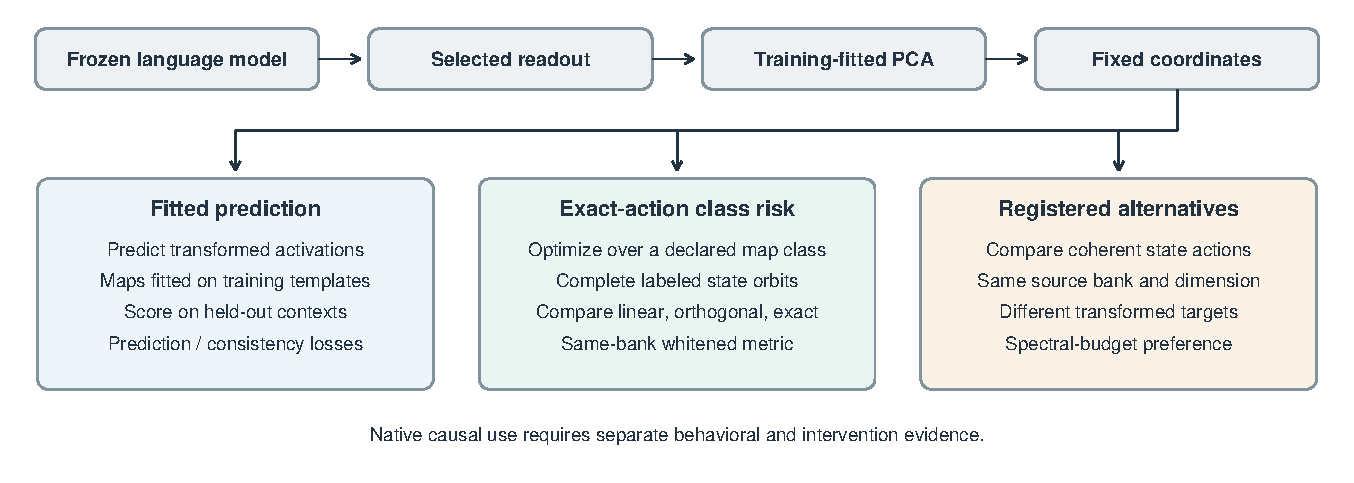
\includegraphics[width=\textwidth]{figures/evaluation_targets.pdf}
\caption{Three questions from the same fixed representations. Fitted prediction evaluates learned maps on held-out contexts; exact-action analysis bounds an optimum in a declared class and metric; registration comparisons change the coherent target action while keeping the source bank fixed. The parallel branches are not a chain of implications toward semantic or causal identification.}
\label{fig:evaluation-targets}
\end{figure}

\section{Related Work}
\label{sec:related-main}
\paragraph{Recovering transformations in representations.}
Paired-map fitting measures input transformations through maps between representations and supports network stitching \citep{lenc2015understanding}. Sun studies when transformations descend through an encoder, when context-wise realizations share a map, and the resulting prediction errors \citep{sun2026transformationlaws}. Homomorphism errors also diagnose compositional generalization \citep{an2026homomorphism}. These works motivate our observation model. Our theoretical target is the optimum over an entire exact orthogonal-action class, rather than the error of a fitted map.

\paragraph{Learning equivariant representations.}
Homomorphism AutoEncoder jointly learns encodings and action representations from transitions \citep{keurti2023homomorphism}; Equivariance by Contrast establishes identification results for jointly learned coordinates and actions under explicit assumptions \citep{schmidt2025equivariance}. Neural Fourier Transform connects equivariant features to invariant kernels and studies the selection of irreducible components under a finite latent-dimension budget \citep{koyama2024fourier}. Its objective reconstructs observations through learned encoders and decoders. \citet{ordonez2026inference} learn features for finite-rank Hilbert--Schmidt approximation of a conditional expectation operator, with symmetry-compatible spectral truncation and statistical learning guarantees. These are direct precedents for using representation types in spectral learning. Here the observed coordinates and metric are fixed, the labeled input action is supplied, and the optimized objects are $r\times r$ action matrices predicting transformed observations. We do not optimize an encoder, a decoder or a conditional-probability model.

\paragraph{Invariant approximation and representation constraints.}
Orbit Gram spectra support best group-invariant approximation \citep{barbieri2020approximation}, while real representation theory constrains admissible dimensions \citep{serre1977linear}. Compression, polar decomposition and intertwiner averaging also underlie approximate-representation results \citep{moore2015approximate,gowers2017inverse}. Our bound connects invariant approximation to prediction risk over the exact $O(r)$ action class. Its budget is total real dimension, rather than the number of orbit generators, and its loss measures transformed observations, rather than multiplication defects. The independent orthogonal comparator uses standard Procrustes optimization to separate orthogonality cost from bounds on the additional common-law cost.

\paragraph{Approximation cost and generalization.}
Symmetry constraints can incur prediction error when they mismatch the target. \citet{wang2023equivariance} bound regression error with prescribed input and output actions, optimizing the equivariant predictor. We instead hold observations fixed and optimize the output action itself over the declared class. Conversely, \citet{elesedy2021generalisation} quantify finite-sample generalization gains when the target obeys the assumed symmetry. An increased class-optimal approximation risk therefore does not imply worse generalization for every fitted constrained estimator. Our finite-bank bounds quantify a fixed loss target; they do not supply the sampling guarantees of symmetry-aware representation learning \citep{ordonez2026inference}.

\paragraph{Interpreting predictive structure.}
Calendar features and their causal use have been studied in language models \citep{engels2025notall}; modular-addition and group-operation studies examine computations in networks trained on those tasks \citep{nanda2023progress,chughtai2023toy,wu2025unified}. Our inputs already name the state, so prediction tests a representational relation. Probe controls distinguish representation properties from an external predictor's capabilities \citep{hewitt2019designing}, while causal abstraction requires intervention evidence for computational interpretations \citep{geiger2022inducing,geiger2025causal}. Our category and registration controls compare explanations of predictive relations. The class-risk bound quantifies compatibility with exact actions; neither comparison establishes native computation. \Cref{app:related-work} details the differences in assumptions and objectives.

\section{Problem Setup and Evaluation Targets}
\label{sec:setup}
\subsection{Paired states in fixed coordinates}
Let $S$ be a finite set of $n$ states and $G$ a prescribed finite group acting on $S$ by permutations. For a state $i\in S$, an element $g\in G$ produces state $g(i)$. A contextual template $t\in\mathcal T_{\mathrm{tpl}}$ supplies the surrounding text. Thus a source--target pair changes the state while keeping its context fixed. We use the cyclic group $C_7$ of order seven for weekday shifts and the dihedral group $D_4$ of order eight for rotations and reflections of NW, NE, SE and SW. The latter has four states but eight distinct permutations. Each corner is fixed by two elements, so this action is faithful but not free.

Fix a domain, model, layer and data split, with training templates $\mathcal T_{\mathrm{train}}\subset\mathcal T_{\mathrm{tpl}}$. The hidden readout $h_{i,t}\in\R^{1\times d}$ has the model's hidden dimension $d$. It is obtained by averaging the selected layer's block outputs over token positions overlapping the unique state occurrence. It represents a state visible in the input. To define one coordinate system for all contexts, we estimate the mean on the complete training state--template product and retain $q$ principal components:
\[
 \hat\mu=\frac{1}{n|\mathcal T_{\mathrm{train}}|}
 \sum_{t\in\mathcal T_{\mathrm{train}}}\sum_{i\in S}h_{i,t}
 \in\R^{1\times d},
\]
\begin{equation}
 z_{i,t}=(h_{i,t}-\hat\mu)U_{\mathrm{PCA}}\in\R^{1\times q},
 \qquad U_{\mathrm{PCA}}^\top U_{\mathrm{PCA}}=I_q.
 \label{eq:projection}
\end{equation}
Here $U_{\mathrm{PCA}}\in\R^{d\times q}$ contains the leading eigenvectors of the centered training covariance. The principal component analysis (PCA) scores $z_{i,t}$ reconstruct $\hat h_{i,t}=\hat\mu+z_{i,t}U_{\mathrm{PCA}}^\top$; they omit the residual outside the retained subspace. Mean and basis remain fixed on validation and test templates. They are fitted separately across domains, models, layers and splits. PCA here centers and projects; the second-moment whitening used for class-risk analysis is a separate operation.

The primary retained dimension is $q=16$, a fixed analysis setting whose original selection rationale is not recoverable from the available records. It is not an intrinsic-dimension estimate or an established optimum. We also examine the leading eight saved coordinates. The lexical comparison instead matches the ranks of \emph{training projected representations} at $q=6$ for weekdays and $q=3$ for corners. Centering $n$ unique lexical vectors gives only the upper bound $n-1$; equality here is supported by audited input spectra and the recorded PCA procedure. Historical projected arrays are missing for direct output remeasurement. Retained dimension, training-data rank, coordinate-bank rank and operator rank remain distinct, and matching rank does not match retained information. The rank evidence is documented in \cref{app:dimension-rank-audit}.

\subsection{What a fitted operator predicts}
For each element $g$, we fit a matrix $R_g\in\R^{q\times q}$ with the prediction target
\begin{equation}
 z_{i,t}R_g\approx z_{g(i),t}.
 \label{eq:prediction}
\end{equation}
The same family acts across contexts within the fixed coordinate space above; there is no context-specific realignment or matrix shared across models. Both PCA and operator fitting use training templates. Holding out a template holds out its complete set of state variants, while the state vocabulary remains familiar.

Independent ridge fits the element matrices separately. Joint fitting optimizes them together with soft prediction, homomorphism, relation, identity and orthogonality terms. These penalties encourage consistency without enforcing an exact orthogonal action. Under our row-vector convention, applying $g_2$ and then $g_1$ corresponds to
\begin{equation}
 R_{g_2}R_{g_1}\approx R_{g_1\circ g_2},
 \qquad (g_1\circ g_2)(i)=g_1(g_2(i)).
 \label{eq:convention}
\end{equation}
The first matrix is on the left because row vectors multiply on the right. Generator-only fitting supervises the one-day shift for $C_7$, or the clockwise quarter-turn and the reflection swapping NW/NE and SW/SE for $D_4$. For a fixed word $g=g_1\circ\cdots\circ g_k$, it predicts with $R_{g_k}\cdots R_{g_1}$. An exact action assigns equivalent words the same matrix; an approximate fit need not. Its transfer test compares these products with actual transformed activations, not merely with other fitted matrices.

The structural study evaluates paired row matrices $A,B\in\R^{N\times q}$ using
\begin{equation}
 D(A,B)=\frac1N\sum_{j=1}^{N}
 \frac{\|A_j-B_j\|_2^2}{\|B_j\|_2^2+10^{-12}}.
 \label{eq:D}
\end{equation}
This is a mean squared error relative to each target row's energy; zero means exact prediction. It is not an accuracy percentage or a root-mean-square error. Stack one template's source states in $Z$ and its ordered targets in $Z_g$. Prediction error $\Eeq$ averages $D(ZR_g,Z_g)$ over nonidentity elements. Consistency error $\Ehom$ instead averages $D(ZR_{g_2}R_{g_1},ZR_{g_1\circ g_2})$ over element pairs; $\Ecomp$ excludes pairs containing identity. The latter two compare composed and fitted predictions. Because prediction residuals and operator norms also constrain composition residuals, good consistency is not automatically additional identification evidence. Data-space relation diagnostics likewise use $D$; operator-space diagnostics instead use unsquared relative Frobenius norms. The definitions are given in \cref{app:metrics}.

\subsection{From a fitted predictor to an action class}
To compare constraints on the same scale, write the observations as $z_{c,s}\in\R^{1\times r}$, with context $c$ and state $s$. Fix a context distribution $P_C$ and use uniform states and a full uniform group average, including identity and fixed points. Assume the uncentered second moment is positive definite, and whiten it:
\[
 \Sigma=\mathbb E[z^\top z]\succ0,\qquad
 x=z\Sigma^{-1/2},\qquad x_g(c,s)=x(c,g(s)),\qquad
 \mathbb E[x^\top x]=I_r.
\]
For a finite coordinate bank the expectations are its empirical averages. We take $r=q$ only when the stated nonsingularity condition holds. A deficient bank would define a different problem if its dimension or whitening were changed; it is not silently repaired here.

For matrices $A_g\in\R^{r\times r}$, use the common prediction loss
\begin{equation}
 \mathcal L((A_g)_g)=\frac{1}{r|G|}\sum_{g\in G}
 \mathbb E\|xA_g-x_g\|_2^2.
 \label{eq:class-loss-main}
\end{equation}
Allowing each $A_g$ to be any real matrix gives the ordinary least-squares optimum $\eta$. Requiring each matrix to be orthogonal gives $L_{\mathrm{orth}}$, but still permits unrelated choices for different elements. Finally require one exact row action,
\[
 \mathcal R_r(G)=\{\rho:G\to O(r):\rho_e=I_r,\ \rho_g\rho_h=\rho_{hg}\},
\]
and denote its optimum by $L^\star$. Here $gh$ means first $h$, then $g$, so the reversed matrix order is the convention in \cref{eq:convention}. The three targets are
\[
 \eta=\inf_{(A_g)_g}\mathcal L((A_g)_g),\qquad
 L_{\mathrm{orth}}=\inf_{Q_g\in O(r)}\mathcal L((Q_g)_g),\qquad
 L^\star=\inf_{\rho\in\mathcal R_r(G)}\mathcal L(\rho),
\]
Each successive class adds a constraint, so $\eta\le L_{\mathrm{orth}}\le L^\star$. Their differences therefore measure costs within one distribution and metric. A training-fitted predictor's held-out loss is another target: its matrices and training metric remain fixed while the evaluation observations change. We use OLS for ordinary least squares below.

The third research question changes the target action itself. A \emph{registration} assigns the prescribed transformations to the labeled states. A coherent alternative, such as conjugating the weekday cycle by a state-label swap, keeps group laws but changes which state is the target of each transformation. We compare distinct permutation-image subgroups on the same source bank. The spectral budget introduced next measures each candidate's compatibility with the exact-action class. It does not turn these different registered tasks into identical-target predictor comparisons.

\begin{table}[t]
\centering\small
\begin{tabular}{@{}p{.19\textwidth}p{.40\textwidth}p{.33\textwidth}@{}}
\toprule
Target & Loss / normalization & Interpretation \\
\midrule
{\raggedright Structural prediction and consistency\par} & $D(A,B)$: squared error divided by each target row's squared norm & Fitted maps in Study~1; the target depends on the endpoint. \\
Coordinate prediction & Squared error divided by $E_z=\mathbb E_{\rm train}\|z-\bar z_{\rm train}\|_2^2$ & Study~2 predictors; training-only energy denominator. \\
{\raggedright Context-difference transport\par} & Squared error divided by $E_u=\mathbb E_{\rm train}\|u\|_2^2$, where $u$ is the difference between paired same-state contexts & Study~2 difference prediction; no extra recentering. \\
Action-class risks & $\mathcal L$ in \cref{eq:class-loss-main}: second-moment whitening, division by $r$, full group average & $\eta,L_{\rm orth},L^\star$ on the same distribution; bank bounds use its own metric. \\
{\raggedright Constructed-action transfer\par} & The same squared loss form, retaining training whitening and fitted maps & A particular predictor on a new bank, not that bank's class optimum. \\
\bottomrule
\end{tabular}
\caption{Targets used in the experiments. The denominators and prediction objects differ across rows, so their numerical values are not directly comparable. In the spectral analysis, the action dimension $r$ equals retained dimension $q$ in a nonsingular bank.}
\label{tab:metric-contract}
\end{table}

\section{Exact-Action Risk: A Type-Constrained Spectral Characterization}
\label{sec:boundaries}
The optimum $\eta$ answers how accurately unrelated linear maps can predict the transformed observations. It does not tell us how much accuracy must be sacrificed to use one exact orthogonal action. We first show what information is missing, then construct a spectral quantity that bounds $L^\star$. Throughout this section the coordinates are fixed, states and group elements are averaged uniformly, and the uncentered second moment is positive definite, as specified in \cref{sec:setup}.

\subsection{Equal regression risks can hide different action costs}
Consider $G=S=C_2\times C_2\times C_7$ acting by addition on uniform states $(a,b,k)$. There is one context and the observation dimension is $r=1$. Define
\[
 x_A=\frac{(-1)^a+(-1)^b}{\sqrt2},\qquad
 x_B=\sqrt2\cos(2\pi k/7).
\]
Both observations have unit second moment. Both also give optimal independent linear risk $\eta=1/2$ and nonzero orbit-Gram eigenvalues $\{1/2,1/2\}$. Yet their best exact actions have different risks:
\[
 \boxed{L_A^\star=1,\qquad L_B^\star=2.}
\]
The missing information is the type of variation represented by the two equal eigenvalues. In $A$, each component is a real one-dimensional character. In $B$, the two components form a single two-dimensional rotation representation. A one-dimensional action can retain one character, but cannot retain half of a rotation plane. Ordinary eigenvalues report energy without this dimension constraint. The example separates summaries of the observations, not identical full observation distributions; the labeled systems themselves are different. Its complete calculation is given in \cref{sp:counterexample}.

\subsection{Measuring energy under an invariant-dimension budget}
To retain the information omitted by the ordinary spectrum, we use both the orbit observations and their known group action. For each context--state pair, concatenate all transformed whitened coordinates:
\begin{equation}
 v(c,s)=|G|^{-1/2}(x(c,g(s)))_{g\in G}\in\R^{1\times r|G|},
 \qquad K=\mathbb E[v^\top v].
 \label{eq:orbit-gram-main}
\end{equation}
The orbit Gram matrix $K$ is an $r|G|\times r|G|$ positive-semidefinite matrix with trace $r$. Its $(g,h)$ block is $|G|^{-1}\mathbb E[x_g^\top x_h]$, so it records cross-moments between complete transformed observations. On a finite bank, this construction uses the recorded complete state blocks, not a fitted predictor's outputs.

The group also acts on the block indices. For a block vector $a=(a_k)_{k\in G}$, define $(\Lambda_g a)_k=a_{kg^{-1}}$. Uniform state averaging makes $K$ commute with these block permutations. This known action tells us which subspaces are invariant. We seek the invariant subspace that captures the most orbit energy using at most $r$ real dimensions:
\begin{equation}
 \gamma_r=\frac{C_r(K)}r,\qquad
 C_r(K)=\max_Q\operatorname{tr}(KQ),\quad
 \begin{gathered}
 Q^2=Q=Q^\top,\quad Q\Lambda_g=\Lambda_gQ\quad(\forall g),\\
 \operatorname{rank}Q\le r,\quad\operatorname{range}Q\subseteq\operatorname{range}K.
 \end{gathered}
 \label{eq:budget-main}
\end{equation}
Here $Q$ is the projection onto the selected subspace. Commutation enforces invariance, the rank constraint imposes the dimension budget, and $\operatorname{tr}(KQ)$ is its captured energy. Division by the total energy $r$ gives $0\le\gamma_r\le1$.

The optimization has a useful representation-theoretic interpretation. Decompose the known block action into real irreducible types. A copy of type $\tau$ costs $d_\tau$ real dimensions and contributes $d_\tau\lambda$, where $\lambda$ is its multiplicity-operator eigenvalue. Select complete copies whose dimensions sum to at most $r$. For $C_7$, a nontrivial real rotation plane costs two dimensions; choosing a single coordinate from it is not allowed. Thus taking the largest $r$ ordinary eigenvalues can overestimate the feasible energy. We measure that difference by
\[
 \Delta_{\rm type}:=\sum_{j=1}^{r}\lambda_j(K)-C_r(K),
 \qquad \lambda_1(K)\ge\lambda_2(K)\ge\cdots.
\]
In contrast, independent regression depends only on $\eta=1-\operatorname{tr}(K^2)/r$. The pair $(K,\Lambda)$ supplies the type information needed by the budget, while this scalar regression summary discards it. The finite formulation and its invariant-approximation equivalent are established in \cref{sp:budget,sp:observable}.

\subsection{From the budget to risk and constraint costs}
For a finite group acting on complete states under the fixed-coordinate and whitening assumptions above, the budget controls the entire exact orthogonal-action class:
\begin{equation}
 \boxed{2(1-\gamma_r)\le L^\star\le2(1-\gamma_r^2).}
 \label{eq:main-risk-bound}
\end{equation}
The lower endpoint applies to every member of $\mathcal R_r(G)$. The upper endpoint guarantees that at least one member of that same $r$-dimensional class attains it or a smaller risk; it is not a guarantee for every constructed action. When $\gamma_r<1$, the ratio of endpoints is $1+\gamma_r\le2$, and both are zero at $\gamma_r=1$.

The proof relates prediction to invariant approximation. Averaging the observation map against a candidate action produces an intertwiner: a map that respects the two group actions. Its image is a group-invariant subspace of dimension at most $r$, which may contain nontrivial types. The spectral budget bounds its alignment with the observations. Conversely, an optimal invariant subspace, supplemented by auxiliary trivial directions when needed and orthogonally aligned with the observations, induces an admissible $r$-dimensional action with controlled risk. These auxiliary directions change neither the observed data nor the final predictor dimension. This is why the result concerns the whole class rather than the output of a particular fit. \Cref{sp:main} provides the full proof.

\paragraph{The combined cost of exact laws and orthogonality.}
Subtracting the independent linear optimum puts the class restriction on an interpretable scale:
\begin{equation}
 p^-:=\max\{0,2(1-\gamma_r)-\eta\}
 \le L^\star-\eta\le
 p^+:=2(1-\gamma_r^2)-\eta.
 \label{eq:risk-premium-main}
\end{equation}
These endpoints bound the extra error required by both constraints jointly. They are not measured values of the unknown optimum. Their magnitude is more informative than positivity alone, because the same identities imply
\begin{equation}
 \gamma_r\le\sqrt{1-\eta},\qquad
 p^-\ge(1-\sqrt{1-\eta})^2.
 \label{eq:positivity-main}
\end{equation}
Thus $\eta>0$ already entails a positive mathematical lower endpoint. This consequence helps interpret the data; it is not a separate discovery that every imperfect regression yields a positive premium.

\paragraph{How much does orthogonality alone explain?}
Let $M_g=\mathbb E[x^\top x_g]$. Standard orthogonal Procrustes optimization gives the independently orthogonal optimum and its cost relative to linear regression:
\[
 L_{\mathrm{orth}}=2-\frac{2}{r|G|}\sum_g\|M_g\|_*,\qquad
 \beta=L_{\mathrm{orth}}-\eta,
\]
where the nuclear norm $\|M_g\|_*$ sums its singular values. Each element may choose its own matrix in $O(r)$, including reflections, without satisfying common group laws. The joint cost then separates as
\begin{align*}
 L^\star-\eta&=\beta+(L^\star-L_{\mathrm{orth}}),\\
 \ell^-:=\max\{0,2(1-\gamma_r)-L_{\mathrm{orth}}\}
 &\le L^\star-L_{\mathrm{orth}}\le
 \ell^+:=2(1-\gamma_r^2)-L_{\mathrm{orth}}.
\end{align*}
The directly computed $\beta$ measures orthogonality cost. The interval $[\ell^-,\ell^+]$ bounds the further cost of requiring the orthogonal family to obey the common group law. True costs add, but clipped lower endpoints need not: in general $p^-\ne\beta+\ell^-$. Neither a ratio such as $\beta/p^-$ nor the concentration of lower endpoints measures how the unknown true cost is allocated. The positivity and Procrustes derivations are in \cref{sp:premium-positivity,sp:orthogonal-comparator}.

The additional law cost is zero exactly when the independently optimal orthogonal maps admit a choice satisfying the row-action laws. If every $M_g$ is nonsingular, its orthogonal polar factor is unique, so this criterion reduces to checking that one family. With singular cross-moments, failure of an arbitrary SVD completion is inconclusive: another optimal choice may obey the laws (\cref{sp:orthogonal-compatibility}). This is an exact compatibility criterion, not a guarantee inferred from a small numerical residual.

The two observation systems above separate the costs explicitly. With
$a_7=\frac17\sum_{k=0}^6|\cos(2\pi k/7)|$, their risks satisfy
\[
\begin{array}{c|ccc}
 & L_{\mathrm{orth}} & L_{\mathrm{orth}}-\eta & L^\star-L_{\mathrm{orth}}\\
 \hline
 A & 1 & 1/2 & 0\\
 B & 2-2a_7 & 3/2-2a_7 & 2a_7
\end{array}
\]
System $A$ admits a compatible optimal choice despite singular cross-moments. In $B$, the unique polar signs violate the cycle law, creating an additional cost. These are exact calculations for the analytical example; \cref{sp:counterexample} gives the derivation.

\paragraph{An identity reference in the same metric.}
A simple admissible family assigns $\rho_g=I_r$ to \emph{every} element, predicting no change for any transformation. Its risk is
\begin{equation}
 L(I)=\mathcal L((I_r)_{g\in G})=2(1-e_{\rm triv}),
 \qquad
 e_{\rm triv}=\frac1r\mathbb E\left\|\frac1{|G|}\sum_{g\in G}x_g\right\|_2^2.
 \label{eq:identity-reference-main}
\end{equation}
This evaluates the identity \emph{family}, not just the identity group element, whose target is unchanged. The group average extracts the state-invariant component. For our transitive weekday and corner actions it is the within-context state mean. The quantity $e_{\rm triv}$ counts all this trivial-type energy, whereas $b_{\rm triv}$ counts only the trivial-type energy selected by the maximizing dimension budget, also divided by $r$. They can differ because the budget must allocate dimensions among types. The identity-risk formula supplies a same-metric reference for the empirical class bounds (\cref{sp:identity-reference}).

\paragraph{What the calculation establishes.}
For a complete finite bank, these formulas give deterministic bounds on its exact $O(r)$ action optimum. A high budget guarantees compatibility in that declared metric. It does not select a unique semantic registration: centered affinely independent category vectors already admit every state permutation, and stable state coding can support one action across contexts. Likewise, composition residuals are coupled to predictive residuals and operator norms. The finite-orbit and error-propagation results make these alternatives explicit (\cref{prop:finite,prop:propagation}).

The class is exact orthogonal actions after the specified whitening, not all invertible or nonlinear actions. Ordinary ridge and soft-penalty Joint therefore need not belong to it. Conjugating an action into another whitening coordinate system preserves its group law but can change Euclidean orthogonality; this matters when comparing the bank bounds with transfer below. Finally, the finite-bank calculation is not a population certificate. The separate finite-context certificate requires a sampling contract unmet by this fixed panel (\cref{sp:certificate}).

\section{Experiments}
\label{sec:pending-studies}
\label{sec:evidence}
The experiments follow the distinction between a predictor, an action class and a registration. We first establish what fitted maps predict and which simpler explanations compete with them. We then measure exact-action costs on complete banks, evaluate the transfer of a particular constructed action, and compare coherent registrations. A final context-transport study tests the reach of a predictive fitting objective under a new language construction.

\subsection{Models, coordinate banks, and evaluation design}
\label{sec:design}
We analyze six frozen, pretrained decoder-only autoregressive Transformers: Llama-3.2-1B/3B, Llama-3.1-8B and Qwen2.5-1.5B/3B/7B. Four normalized depth slots, $0.2,0.4,0.6,0.8$, give 24 model/readout conditions per domain. Each has its own training-derived coordinate system and operator family. The primary coordinate dimension is 16; the spectral sensitivity comparison uses the first eight coordinates of the same saved PCA. The C7/D4 states are visible input words throughout these evaluations.

The data constructions serve different purposes. The structural-recovery bank (Study~1) contains 40 short templates per domain. Each of five seeded partitions allocates 28 to training, six to diagnostic validation and six to testing, keeping all states of a template together. The coordinate bank (Study~2) uses a separate grammar construction with 48 training, 16 validation and 64 test families, each comprising two paired variants and complete state sets. Its test bank therefore contains 128 complete state blocks per condition. Those blocks support both predictor evaluation and the finite-bank spectral calculation, with different losses. A further 64-family authored bank is reserved for the context-transport comparison. Prompt lists, model revisions and exact partitions are retained with the methods and bank definitions (\cref{app:methods,app:characterization,app:pending-protocols}).

\hypertarget{par:estimation}{}
Study~1 ridge fits no-intercept maps with coefficient $0.01$. Joint starts from these maps and uses AdamW to optimize the small matrices with soft prediction and algebraic penalties; the language model stays frozen. Generator-only fitting withholds supervision for nongenerator elements. Study~2 uses the recorded training and validation rules for each predictor, and all transfer evaluations keep their fitted coordinates fixed. For class-risk analysis, by contrast, the evaluated bank itself defines the observation distribution and second-moment metric. Including identity elements and fixed points is part of that full-group target. Optimization parameters remain in one implementation specification (\cref{app:methods}).

All spectral means give equal weight to the 24 conditions in a domain and dimension; the orthogonal comparison includes all 96 domain/dimension/condition units. These models and readouts form a selected panel, and Study~1's five overlapping partitions are not five independent datasets. Reported bootstrap ranges describe sensitivity under the recorded resampling scheme, rather than calibrated population coverage. In the new-context comparison the unit is a paired family, retaining its measurements across models, readouts and domains together. Counts of winning conditions are descriptive panel summaries. The complete resampling rules are in \cref{app:inference,app:pending-protocols}.

\subsection{Predictive recovery and competing explanations}
\label{sec:characterization}
\paragraph{Shared maps predict familiar transformations.}
Independent ridge predicts held-out Study~1 representations with mean $\Eeq=0.04830$ for C7 and $0.05200$ for D4. Joint yields $0.04934$ and $0.05286$: encouraging group structure does not improve this direct-prediction endpoint. It does reduce the recorded relation defects, which test generator powers and inverse/composition relations. Predictive fit and algebraic consistency can therefore respond differently to the objective, while remaining mathematically coupled through prediction residuals and operator norms.

With only generator supervision, matrix products predict five excluded nonidentity elements in each group. Their errors are $0.074443/0.056558$ for C7/D4; directly fitting those same elements in that comparison gives $0.051124/0.050032$. This is transfer across the requested action, as well as across held-out templates, but not across an unseen state vocabulary. It establishes useful predictive composition without requiring that the fitted family be an exact action. Detailed structural endpoints are in \cref{app:results}.

\paragraph{Category information provides a competitive explanation.}
The two-model lexical comparison gives near-exact fits for lexical embeddings and larger errors for internal representations at matched training projected ranks $q=6/3$. This is consistent with the finite-orbit result: generic category vectors already support every state permutation. Equal projected rank does not equalize the amount or kind of retained information.

A stronger Study~2 control makes category information explicit. It decodes the source state by its nearest training centroid and shifts the source by the difference between target and source centroids. In the equal-action compact comparison, its mean losses are $0.012013/0.063821$, versus ridge's $0.014897/0.041919$. The centroid predictor wins in 9/24 C7 and 2/24 D4 conditions: its better weekday mean is not a uniform improvement. It receives construction state labels and the exact action table, which the source-coordinate/action predictors do not. Its competitiveness demonstrates an available predictive explanation under extra information, rather than a matched-supervision victory over ridge.

Capacity also changes the comparison. Random Fourier feature (RFF) and Nystr\"om predictors fit the target-minus-source displacement from all construction target pairs, then add it to the source. Neither improves both domain means at the linear storage budget with the identity map omitted from storage; Nystr\"om does at $2\times$ storage and RFF at $4\times$. This budget counts predictor parameters, features, normalizers and lookup data, excluding shared PCA, model weights and runtime memory. The result is a ranking under stated information and storage conditions, not universal linear superiority. Nor does nonlinear predictive accuracy establish a nonlinear group action. The complete budget curves and comparator definitions are in \cref{app:reproduction}.

\paragraph{A coherent alternative survives a different control.}
Corrupting training correspondences and refitting ridge worsens prediction of the unchanged true test targets. That shows dependence on supervision. Conjugating the action by a fixed state-label swap instead defines another consistent task, preserving group laws and fixed-point counts. Ridge losses for specified/alternative correspondences are $0.014897/0.017503$ for C7 and $0.041919/0.041871$ for D4. They use the same source bank but different targets and registration-specific changed-state masks. The alternative's competitive prediction motivates asking how exceptional the prescribed action is among \emph{all} images in the declared comparator class. The original disruption and coherent-action controls are detailed in \cref{app:predictive-controls,app:reproduction}.

These comparisons concern fitted predictors. They lead to a different question: what error is unavoidable for any exact orthogonal action in the same retained space? An algebraic penalty or a competitive category baseline cannot answer that class-level question.

\subsection{Exact-action cost in observed representation banks}
\label{sec:observed-risk}
% Presentation only: select and round previously saved means.
\begin{table*}[t]
\centering\small
\setlength{\tabcolsep}{4pt}
\textbf{(a) Joint constraint cost, $r=16$}\par\smallskip
\begin{tabular}{@{}lrrrr@{}}
\toprule
Domain & Mean $\eta$ & Mean $L^\star$ bounds & Mean $L^\star-\eta$ bounds & Mean $L(I)$ \\
\midrule
$C_7$ & 0.02563 & [0.02980, 0.05863] & [0.00416, 0.03300] & 0.76012 \\
$D_4$ & 0.10321 & [0.12944, 0.24895] & [0.02624, 0.14574] & 0.52932 \\
\bottomrule
\end{tabular}
\par\medskip
\textbf{(b) Independent orthogonality and further group-law cost}\par\smallskip
\begin{tabular}{@{}rlrrrr@{}}
\toprule
$r$ & Domain & Mean $L_{\rm orth}$ & Mean $\beta$ & Mean $L^\star-L_{\rm orth}$ bounds & $\ell^->\tau$ \\
\midrule
16 & $C_7$ & 0.028706 & 0.003074 & [0.001097, 0.029927] & 23/24 \\
16 & $D_4$ & 0.127737 & 0.024531 & [0.001842, 0.121209] & 23/24 \\
8 & $C_7$ & 0.096717 & 0.029571 & [0.035397, 0.151842] & 22/24 \\
8 & $D_4$ & 0.080819 & 0.010217 & [0.000052, 0.076930] & 19/24 \\
\bottomrule
\end{tabular}
\caption{\textbf{Same-bank risks and constraint costs.} Each row averages all 24 fixed model/readout conditions on the Study~2 test banks. Panel (a) bounds the joint cost of exact laws and orthogonality; panel (b) separates the computed orthogonality cost $\beta$ from bounds on further common-law cost. Endpoints are computed per condition before averaging. The last column uses the fixed tolerance $\tau=10^{-8}+10^{-7}|\ell^-|$. Intervals bound mean class optima; they are not confidence intervals or measured optima. Each dimension uses its own second-moment-whitened metric.}
\label{tab:core-risk-summary}
\end{table*}

\begin{figure}[t]
\centering
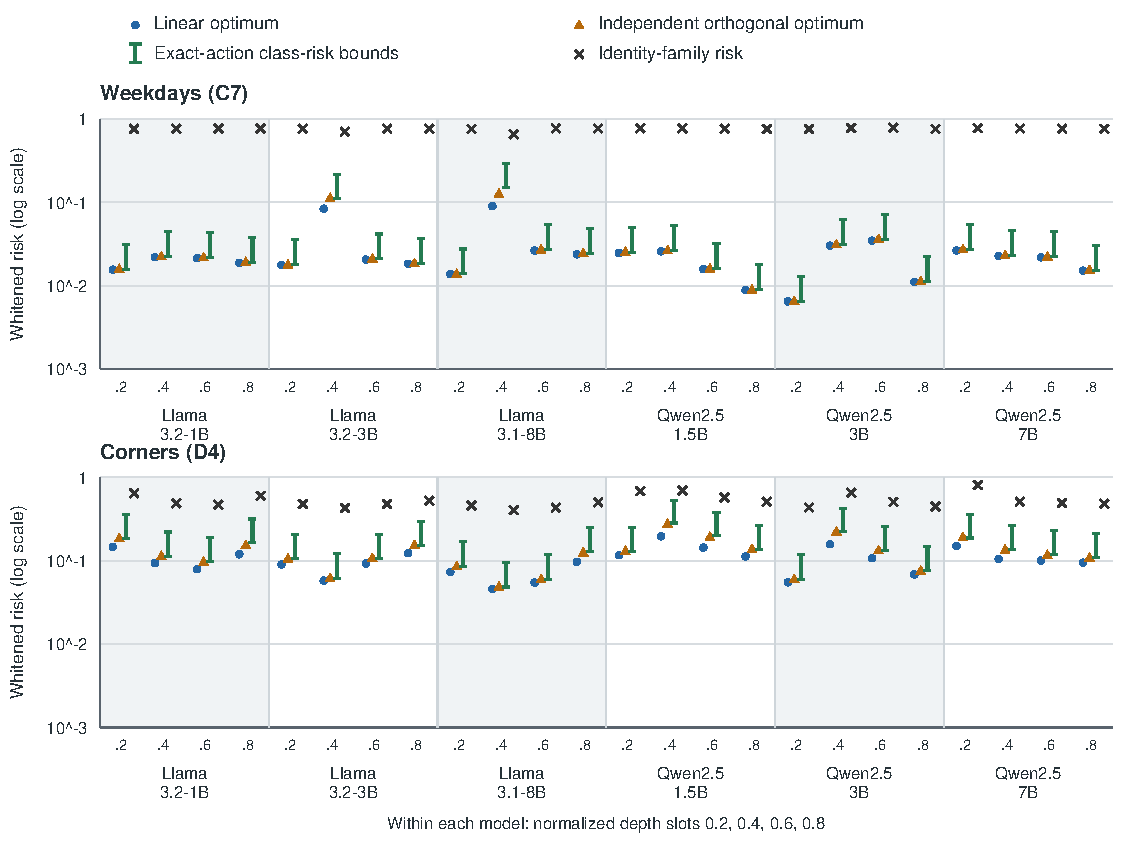
\includegraphics[width=\textwidth]{figures/same_metric_risks_v061.pdf}
\caption{\textbf{Same-metric risks in every primary condition.} Circles show $\eta$, triangles $L_{\rm orth}$, green segments $[2(1-\gamma_r),2(1-\gamma_r^2)]$, and crosses $L(I)$ at $r=16$. Within each of the 48 conditions, all four quantities use the same complete Study~2 test bank, its own second-moment whitening, and uniform state/group weights. Each model has four readouts; horizontal offsets separate symbols. The logarithmic axis shows absolute risk levels, not additive constraint costs. Segments bound the exact-action class optimum; they are neither confidence intervals nor measured witness losses. All conditions are retained. Training-metric witness transfer is reported separately in \cref{sec:witness-transfer}.}
\label{fig:same-metric-risks}
\end{figure}
We evaluate the class-risk quantities on the complete Study~2 test banks, using each bank's own empirical second moment. These are deterministic characterizations of the observed distributions, not held-out scores of training-fitted predictors. At $r=16$, the mean budgets are $\gamma_r=0.98510/0.93528$ for C7/D4. Table~\ref{tab:core-risk-summary}a bounds the mean exact-action risks by $[0.02980,0.05863]$ and $[0.12944,0.24895]$, compared with independent linear optima of $0.02563/0.10321$. The corresponding identity-family risks are $0.76012/0.52932$. Thus the bounds support substantially better prediction than this no-change reference on average, while quantifying a cost relative to unconstrained linear prediction.

\Cref{fig:same-metric-risks} places these class bounds beside both independent optima and the identity reference in every primary condition. It separates two conclusions that a domain mean can obscure: an exact action can improve on the no-change reference, while imposing exact orthogonality and group laws can still cost accuracy relative to independent prediction. The absolute risks vary across models and readouts; the additive costs and their heterogeneity are quantified below rather than inferred from distances on the logarithmic axis.

\paragraph{The joint cost is heterogeneous.}
For C7, the mean interval for $L^\star-\eta$ is $[\BoundedPremiumLowerCseven,\BoundedPremiumUpperCseven]$, but its lower endpoints have median only $0.000389$ and range $[0.0000349,0.06254]$. Two conditions---Llama-3.1-8B/layer 13 and Llama-3.2-3B/layer 11---contribute $90.7\%$ of their sum. D4 has mean interval $[\BoundedPremiumLowerDfour,\BoundedPremiumUpperDfour]$, lower-endpoint median $0.01876$ and range $[0.00254,0.08719]$. All conditions retain equal weight. The mean is therefore insufficient to describe the weekday guarantees. Moreover, positivity of $p^-$ follows from $\eta>0$ under the theorem; the data inform its magnitude and distribution, not a separate positivity discovery.

\paragraph{Common group laws add a distinct constraint.}
\label{par:orthogonal-results}
Could orthogonality explain the entire joint cost? At $r=16$, independently orthogonal maps have mean $L_{\rm orth}=0.028706/0.127737$, giving $\beta=0.003074/0.024531$. The further common-law cost has mean bounds $[0.001097,0.029927]$ for C7 and $[0.001842,0.121209]$ for D4. Its lower endpoint exceeds the fixed numerical tolerance in 23/24 conditions per domain. Under the stated assumptions and numerical checks, orthogonality alone therefore cannot explain the whole joint cost in those conditions.

The scale of that remaining guarantee is especially uneven in C7. Its $\ell^-$ median is $5.35\times10^{-6}$, with range $[0,0.026188]$; Llama-3.1-8B/layer 13 supplies $99.44\%$ of the lower-endpoint sum. This one-condition concentration concerns the further-law bound, whereas the two-condition $90.7\%$ concentration above concerns the joint bound. Neither is a proportion of the unknown true costs. D4's further-law endpoints have median $0.000339$ and range $[0,0.012617]$. The upper bounds remain much wider, so small lower endpoints do not establish small actual costs.

\paragraph{Sensitivity to individual context families.}
We delete each of the 64 complete C7 families in every $r=16$ condition, removing both variants and their complete seven-state blocks together. All 1,536 deletions are evaluable, and the same 23/24 conditions exceed the original tolerance after every deletion. Llama-3.1-8B/layer 13 retains $\ell^-\in[0.02435,0.02696]$, compared with $0.02619$ on the complete bank, and accounts for $99.38\%$--$99.48\%$ of the lower-endpoint sum. Thus both the positive-bound count and the cross-condition concentration persist across these deletions. PCA remains fixed, but each reduced bank uses its own second-moment whitening: this is sensitivity to the changed empirical distribution and metric, not additive family attribution under a fixed loss. The check does not address joint deletions or shared construction biases (\cref{app:c7-family-influence}).

At $r=8$, orthogonality costs average $0.029571$ for C7 and $0.010217$ for D4. The further-law mean bounds are $[0.035397,0.151842]$ and $[0.000052,0.076930]$, respectively. Positive lower-endpoint counts become 22/24 and 19/24; one C7 endpoint is only $1.55$ times its tolerance. All nine zero endpoints across both dimensions remain included. A zero endpoint is inconclusive about strict positivity. Since each dimension has its own coordinates, whitening and normalization, this comparison characterizes dependence on the retained space rather than selecting a superior dimension. Per-condition results and numerical rules are in \cref{app:orthogonal-results}.

\paragraph{High budgets do not require a semantic computation.}
The selected trivial contributions average $b_{\rm triv}=0.61540/0.72742$: much of the captured energy is invariant to the state action. These are fractions of total whitened energy, not fractions of $\gamma_r$, and need not equal the total trivial energy used by $L(I)$. Invariant components may include contextual or constant structure; state-dependent components can still encode categories. The type correction is also small in most primary conditions: its absolute value is at most $5.33\times10^{-15}$ in 47/48. Only Llama-3.1-8B/C7/layer 13 has a material correction, $\Delta_{\rm type}/16=0.00827$. Thus real-type constraints are essential to the theorem, but their empirical effect at dimension 16 is concentrated. The detailed type decomposition is in \cref{app:bounded-risk-details}.

\subsection{Transfer of constructed exact actions}
\label{sec:witness-transfer}
\begin{table}[t]
\centering\small
\begin{tabular}{@{}lrrrrr@{}}
\toprule
& Construction bank & \multicolumn{3}{c}{Old test bank, frozen training metric} & Witness worse \\
Domain & Witness & Witness & OLS & Ridge & than OLS \\
\midrule
$C_7$ & 0.02906 & 0.02806 & 0.02141 & 0.02141 & 24/24 \\
$D_4$ & 0.11996 & 0.11117 & 0.08878 & 0.08878 & 24/24 \\
\bottomrule
\end{tabular}
\caption{Transfer of frozen predictors at $r=16$ in the training metric. These means use training whitening for both construction and old test banks, including identity and fixed points. OLS and ridge need not obey group laws. The witness is feasible, not claimed optimal. Its transfer loss is not checked against Table~\ref{tab:core-risk-summary}'s test-metric exact-orthogonal bounds: changing whitening can also change admissibility of the same raw-coordinate function (\cref{app:metric-conjugation}).}
\label{tab:followup-witness}
\end{table}

The bounds concern the best member of an entire class on one bank. We next evaluate one concrete member when contexts are held out. For each condition, an exact-action witness is constructed from training contexts with training second-moment whitening, then frozen. All 48 constructions pass the specified numerical action-law and orthogonality checks, and their construction-bank risks lie within the analytic bounds under those checks. This verifies the intended construction numerically; it is not a rigorous floating-point certificate or evidence that the constructor attains the class optimum.

On the held-out bank, witness losses average $0.02806/0.11117$ for C7/D4, compared with $0.02141/0.08878$ for training-fitted OLS. The witness is worse than OLS and fixed-coefficient ridge in every condition (Table~\ref{tab:followup-witness}). Exact algebraic structure is therefore feasible here without improving this constructor's transfer performance. The ordering is empirical: class inclusion on one distribution does not force an ordering between training-fitted predictors on another.

The comparison also uses a different metric from the preceding bank bounds. Both construction and held-out witness losses retain the \emph{training} whitening, whereas Table~\ref{tab:core-risk-summary} characterizes the test bank in its \emph{own} whitening. Re-expressing the training action in test-whitened coordinates preserves its group law by conjugacy, but need not preserve orthogonality. Its transfer error consequently cannot be judged against that test-metric exact-orthogonal class interval. The constructor and coordinate-change derivation are given in \cref{app:pending-protocols,app:metric-conjugation}.

\subsection{Semantic registration and dimensional sensitivity}
\label{sec:registration-sensitivity}
The existence of a compatible action leaves open which action on state labels is preferred. We enumerate all 120 distinct cyclic order-seven permutation-image subgroups on the weekdays and all three dihedral order-eight images on the corners, including the prescribed image. These counts concern image subgroups, not choices of generators or arbitrary inconsistent relabelings. Every candidate defines coherent transformed targets on the same source bank.

At $r=16$, the prescribed image has uniquely highest $\gamma_r$ in 7/24 C7 and 16/24 D4 conditions. To interpret these ranks, we also compare absolute budgets. For the prescribed image $H_0$, let
\[
 d_{\rm top}=\gamma(H_0)-\max_{H\ne H_0}\gamma(H),\qquad
 d_{\rm median}=\gamma(H_0)-\operatorname{median}_{H\ne H_0}\gamma(H).
\]
The median strongest-alternative margin is $-5.52\times10^{-6}$ in C7 and $5.96\times10^{-6}$ in D4 (Table~\ref{tab:bounded-margins}). C7's budget spread across all images has median $3.88\times10^{-5}$ and maximum $4.07\times10^{-4}$, although its semantic rank ranges from first to a tied interval of 102--105 among 120. D4 spans all three ranks, with median spread $1.36\times10^{-4}$ and maximum $0.03984$. Rank changes can therefore accompany small absolute changes, particularly for weekdays. These are spectral-budget comparisons between registered tasks, not exact-$L^\star$ rankings, permutation $p$-values or semantic probabilities.

\begin{table}[t]
\centering\small
% Generated by analysis/main30_bounded_v1/derive.py; never edit numbers.
\begin{tabular}{llrrrc}
\toprule
Domain & Margin & Median & Min. & Max. & U/T/B \\
\midrule
C7 & $d_{\rm top}$ & $-5.52\!\times\!10^{-6}$ & $-3.03\!\times\!10^{-4}$ & $1.97\!\times\!10^{-5}$ & 7/0/17 \\
 & $d_{\rm median}$ & $1.60\!\times\!10^{-6}$ & $-4.13\!\times\!10^{-5}$ & $4.42\!\times\!10^{-5}$ &  \\
D4 & $d_{\rm top}$ & $5.96\!\times\!10^{-6}$ & $-1.23\!\times\!10^{-2}$ & $3.82\!\times\!10^{-2}$ & 16/0/8 \\
 & $d_{\rm median}$ & $1.46\!\times\!10^{-5}$ & $-2.04\!\times\!10^{-3}$ & $3.90\!\times\!10^{-2}$ &  \\
\bottomrule
\end{tabular}

\caption{Registration margins at $r=16$ in all 24 fixed conditions per domain. Positive values favor the prescribed image over the strongest or median alternative. U/T/B counts unique leading, tied leading and behind under the recorded pairwise tolerance. The margins measure spectral-budget differences between coherent target actions.}
\label{tab:bounded-margins}
\end{table}

A shared invariant component does not by itself settle this comparison. All enumerated images are transitive, so their full trivial energy $e_{\rm triv}$ is the same within a fixed bank: the invariant projection is the within-context state mean. Their selected contributions $b_{\rm triv}$ can differ because types compete for the dimension budget. Even a unique leader leaves automorphisms and stable state coding possible. The mechanism controls illustrate that distinction: both a shared-action construction and a stable-code construction have machine-scale noiseless witness loss, while the sampled contextual-orientation construction has smaller budgets. Stable coding is thus a compatible explanation, not a no-action null that a useful diagnostic must reject. These fixed constructions do not calibrate a semantic classifier (\cref{sp:transitive-trivial-energy,tab:followup-simulations}).

% Format-only selection from the completed sensitivity coverage.
\begin{table}[t]
\centering\small
\setlength{\tabcolsep}{5pt}
\begin{tabular}{@{}lrrrr@{}}
\toprule
Domain & $r$ & Mean $\gamma_r$ & Median $p^-$ & Unique leading image \\
\midrule
$C_7$ & 16 & 0.985102 & 0.000389 & 7/24 \\
$C_7$ & 8 & 0.933943 & 0.041288 & 4/24 \\
\addlinespace
$D_4$ & 16 & 0.935278 & 0.018756 & 16/24 \\
$D_4$ & 8 & 0.959581 & 0.005865 & 19/24 \\
\bottomrule
\end{tabular}
\caption{Retained-dimension sensitivity on the same complete Study~2 banks. Each row summarizes all 24 fixed conditions; $p^-$ is the lower endpoint for joint exact-law and orthogonality cost. The last column counts a uniquely highest budget for the specified semantic image among all 120 C7 or three D4 images, using the original tolerance. Eight coordinates are the leading eight saved PCA coordinates. The dimensions have different whitened metrics and normalizations; these are not optimal-dimension comparisons or significance tests. Full values and checks remain in \cref{app:spectral-dimension-sensitivity}.}
\label{tab:sensitivity-main}
\end{table}

Retaining eight rather than sixteen coordinates changes the answer quantitatively (Table~\ref{tab:sensitivity-main}). The prescribed image is uniquely leading in 4/24 C7 and 19/24 D4 conditions, and the C7 type correction exceeds the original comparison tolerance in eight conditions rather than one. No D4 condition exceeds it at either dimension. The lack of a uniform semantic preference persists, but the margins, costs and preferred images depend on the observation space. Each dimension has its own second-moment metric and $1/r$ normalization, so this is not a common-loss contest to choose an optimal dimension. The complete same-bank sensitivity results remain in \cref{app:spectral-dimension-sensitivity}.

\subsection{Context transport under a new language construction}
\label{sec:new-context}
\begin{table}[t]
\centering\small\setlength{\tabcolsep}{3pt}
\begin{tabular}{@{}lrrrrr@{}}
\toprule
& \multicolumn{3}{c}{Mean context-difference loss} & Difference minus & Family sensitivity \\
Panel & Identity & Coordinate fit & Difference fit & coordinate & range \\
\midrule
$C_7$ & 0.04357 & 0.05031 & 0.04448 & -0.00583 & [-0.00668, -0.00501] \\
$D_4$ & 0.16615 & 0.12273 & 0.12892 & +0.00619 & [+0.00397, +0.00841] \\
Equal-domain mean & 0.10486 & 0.08652 & 0.08670 & +0.00018 & [-0.00103, +0.00136] \\
\bottomrule
\end{tabular}
\caption{New authored contexts under matched validation selection. Losses use old-training difference energy. Negative contrasts favor difference fitting. The last column copies the recorded 2.5th/97.5th percentiles from 2,000 paired-family bootstrap draws; it describes conditional sensitivity over 64 authored families, not calibrated population coverage. Model/readout cells and both domains remain paired in each family.}
\label{tab:followup-context}
\end{table}

A separate prediction question is whether an objective that helps within one context construction also helps on new wording. For paired variants $v=0,1$ of a context family $f$, define $u_{i,f}=z_{i,f,0}-z_{i,f,1}$ and its transformed target $u_{g(i),f}$. Coordinate fitting learns a map on $(z_{i,t},z_{g(i),t})$ and applies it to $u$; difference fitting learns directly from $(u_{i,f},u_{g(i),f})$. Both losses divide squared difference error by the original training difference energy $E_u$. Subtracting same-state representations cancels state-only components but retains context main effects, so the target is not a pure state--context interaction.

The new bank contains 64 assistant-authored paired frames per domain, or 896 weekday and 512 corner prompts per model. Both predictors are fitted on the original training families. Their ridge coefficients are selected using the same original-validation context-difference loss, with no fitting or selection on the new bank. The earlier coordinate comparator instead used coordinate-loss selection. A secondary arm retaining that earlier rule has the same domain signs; nevertheless, comparing the old and new primary results changes selection as well as language construction, rather than isolating language alone. This study evaluates predictive transport, not spectral risks or registration rankings on new contexts.

Difference fitting minus coordinate fitting is $-0.005833$ for C7 and $+0.006190$ for D4 on average. It improves 20/24 weekday conditions and only 8/24 corner conditions. Table~\ref{tab:followup-context} also makes the reference choice important: identity has the smallest weekday mean, while both fitted predictors improve on identity for corners. The equal-domain contrast, $+0.000178$, nearly cancels; its recorded family-resampling percentiles are $[-0.001035,+0.001362]$. Neither cancellation nor an interval spanning zero establishes equivalence. The useful answer is domain-specific: fitting differences helps relative to coordinate fitting for weekdays and hurts for corners in this authored construction.

\begin{figure}[t]
\centering
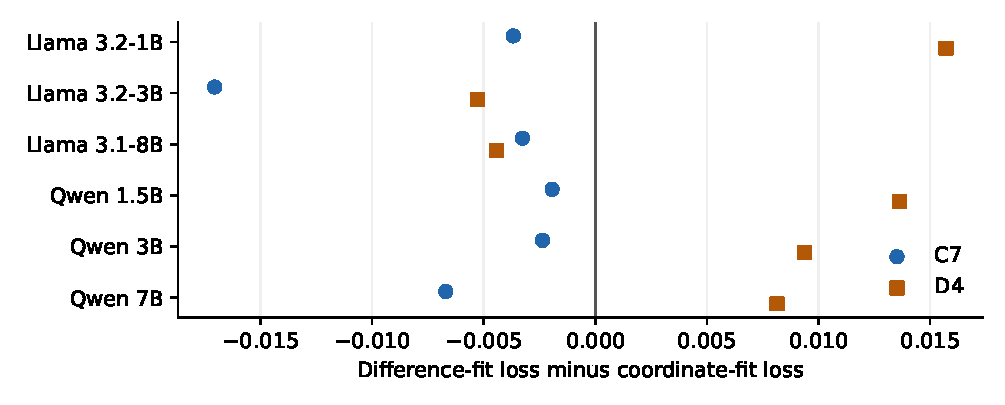
\includegraphics[width=.88\textwidth]{figures/context_transfer_followup.pdf}
\caption{New-context difference-fit minus coordinate-fit loss by model, averaged over four fixed readouts. Negative values favor difference fitting. All six weekday model means are negative, whereas four corner model means are positive. The points summarize the selected panel, not independent population draws; Table~\ref{tab:followup-context} gives the paired-family sensitivity ranges.}
\label{fig:context-followup}
\end{figure}

The frames retain the seen state vocabulary while changing outer narratives and limited factual wording. They are authored pairs, not independent human-prose samples, and only text preceding or overlapping a state span can affect its readout in a causal decoder. The reversal therefore limits a general advantage for difference fitting without identifying a native computation. The exact selection and paired-family resampling contracts are in \cref{app:pending-protocols}.

\section{Discussion and Limitations}
\label{sec:reading-protocol}
The measurements establish more than the existence of a good fitted predictor, but less than a unique account of the model's computation. A computable spectral budget bounds the optimum over an entire exact orthogonal-action class. On the observed representation banks, it quantifies the additional cost of that class and permits a separate comparison with independent orthogonality. This connects a declared structural requirement to a prediction target without requiring a particular construction algorithm to attain the optimum. The constructed witness can therefore be feasible yet transfer worse than OLS without contradicting the class-risk result.

The strongest empirical lesson is that magnitude and variation matter. Positive joint lower endpoints already follow from imperfect independent regression under the theorem's assumptions. The additional group-law bounds provide more specific information, but their primary weekday sum is overwhelmingly concentrated in one condition and their upper bounds leave room for larger true costs. Likewise, the representation-type correction is essential in principle but material in only one primary condition. The complete-family deletion check preserves the primary C7 lower-bound concentration under each reduced bank's own whitening; it does not turn that concentration into evidence of uniformly large costs or replication on new contexts. Eight-coordinate results change its role and change registration rankings. These observations support a conditional characterization of the chosen spaces, not a claim that exact-action cost is uniformly large or dimension-independent.

Coherent registrations also leave plausible alternatives. A state code can realize transformations accurately and a shared invariant component can supply substantial spectral energy. Our complete small-group comparisons ask whether the prescribed image is favored within a declared finite class; even a unique spectral leader would not eliminate every semantic relabeling or identify the generating mechanism. The constructed-action and new-context comparisons add predictive evidence, but the latter concerns transport objectives rather than an independent replication of class risks or registration preferences. Its opposite domain effects further prevent treating difference fitting as a universally better objective.

The scope of the empirical conclusions follows from the observations used. Six selected models and four readouts per model provide repeated measurements, not independent samples of all language models. C7 and D4 contain small, already-seen state vocabularies; the authored-context bank extends wording, not state identities. A supplementary three-object assignment task uses the permutation group $S_3$ with new entity names and contexts; its joint held-out stratum yields only a small transport improvement over identity. Historical activation edits differ in information and intervention space, and the separate native-program branch failed clean-task competence; its confirmation remains blocked (\cref{app:behavior,app:reproduction}). Thus the present evidence does not establish successful native group computation. Finite-bank guarantees also do not supply the sampling assumptions needed for population certification.

For another representation study, the practical distinction is the object of the claim. A held-out prediction score evaluates a trained map; a class-risk bound evaluates structural compatibility under a metric; a registration margin compares coherent target actions. Keeping those objects explicit makes a negative transfer result or a competitive alternative informative rather than an apparent failure of a single recovery score.

\section{Conclusion}
We connect a type-constrained invariant-subspace budget to the minimum prediction risk of fixed-dimensional exact orthogonal actions. In frozen language-model representations, the resulting bounds quantify joint constraint costs and, with an independent orthogonal comparator, delimit the further cost of common group laws. Those guarantees are heterogeneous, constructed actions need not outperform ordinary predictors, and coherent registrations change their spectral ranking across retained spaces. New-context transport adds a separate domain-dependent boundary. Predictive recovery, exact-action compatibility and semantic preference can therefore be measured and compared without treating them as interchangeable evidence of native computation.


\FloatBarrier
\label{sec:main-end}

\section*{Impact Statement}
This work develops diagnostics for interpreting language-model representations. Overinterpreting probes can mislead users about model capabilities or mechanisms. These controlled tasks do not assess demographic fairness or establish safety guarantees. We identify no other specific societal consequences requiring discussion.

\bibliography{references}
\bibliographystyle{tmlr}
% Keep the complete reference list separate from the appendices.
\clearpage
\appendix
\section{Proofs and the Identification Problem}
\label{app:theory}
\label{sec:appendix}
\subsection{Supporting finite-state statements}
The following elementary statements support Section~\ref{sec:boundaries}; they are not presented as new general theory.

\begin{proposition}[Finite-orbit realizability]
\label{prop:finite}
Let $X\in\R^{n\times(n-1)}$ have centered rows and rank $n-1$. For a permutation $g$, define $(P_gX)_i=X_{g(i)}$. There is a unique invertible $R_g=X^\dagger P_gX$ satisfying $XR_g=P_gX$, and $R_gR_h=R_{h\circ g}$.
\end{proposition}

Write $e_g(i,t)=z_{i,t}R_g-z_{g(i),t}$.
\begin{proposition}[Prediction-error propagation]
\label{prop:propagation}
For $p=g_1\circ g_2$, the composition residual is
\begin{align}
 z_{i,t}(R_{g_2}R_{g_1}-R_p)
 &=e_{g_2}(i,t)R_{g_1} \nonumber\\
 &\quad+e_{g_1}(g_2(i),t)-e_p(i,t).
\end{align}
Its norm is at most $\norm{e_{g_2}}_2\norm{R_{g_1}}_{\rm op}+\norm{e_{g_1}(g_2(i),t)}_2+\norm{e_p}_2$.
\end{proposition}

\begin{proposition}[Global-field cancellation]
\label{prop:additive}
For any permutation $g$ of a complete uniformly weighted orbit, $\sum_i(z_{g(i),t}-z_{i,t})=0$. Therefore the train-fitted global displacement $v_g=\mathbb{E}_{i,t}[z_{g(i),t}-z_{i,t}]$ is zero for every element of both tested groups, up to numerical precision.
\end{proposition}

\subsection{Finite-orbit realizability}
\begin{proof}[Proof of \cref{prop:finite}]
Centering implies $\operatorname{col}(X)\subseteq\mathbf{1}^{\perp}$. Both spaces have dimension $n-1$, so they are equal. Every permutation matrix preserves $\mathbf{1}^{\perp}$; hence $P_gX$ lies in the column space of $X$. Full column rank gives the unique solution $R_g=(X^\top X)^{-1}X^\top P_gX$. Our definition implies $P_gP_h=P_{h\circ g}$, and consequently
\[
 XR_gR_h=P_gXR_h=P_gP_hX=P_{h\circ g}X=XR_{h\circ g}.
\]
Uniqueness establishes the multiplication rule. Taking $h=g^{-1}$ proves $R_gR_{g^{-1}}=R_e=\Id$ and the reverse product similarly, so every $R_g$ is invertible.
\end{proof}
If $n$ lexical vectors are affinely independent, their centered span has dimension $n-1$. Keeping all these PCA dimensions makes only an invertible coordinate change, so the proposition still applies. Neither regular polygon geometry nor pretrained knowledge of a named group is required. The induced matrices need not be orthogonal in the measured Euclidean metric. Their exact abstract action and their geometric shape are separate questions.

This interpolation issue also limits representation comparison: invariance to arbitrary invertible changes can make sufficiently high-dimensional sample representations indistinguishable \citep{kornblith2019similarity}. That observation concerns comparison statistics; it does not establish out-of-context transformation prediction.

\subsection{Separate contextual realizations need not be shared}
Consider centered three-state coordinates
\[
 X=\begin{bmatrix}1&0\\0&1\\-1&-1\end{bmatrix},\qquad
 R=\begin{bmatrix}0&1\\-1&-1\end{bmatrix}.
\]
For the cycle $g:1\mapsto2\mapsto3\mapsto1$, $XR=P_gX$. A second contextual copy $Y=XA$, with $A=\operatorname{diag}(2,1)$, has forced operator
\[
 R'=A^{-1}RA=\begin{bmatrix}0&1/2\\-2&-1\end{bmatrix}\ne R.
\]
A shared operator $M$ would satisfy both $XM=P_gX$ and $YM=P_gY$. Full column rank forces $M=R$ from the first and $M=R'$ from the second, a contradiction. This gives a precise reason why training one operator family and evaluating held-out contexts is stronger than recovering a separate action on each finite orbit. The contradiction uses the common fully supported coordinates; unequal extensions on unobserved directions alone would not suffice.

\subsection{Shared contextual realizations can still reflect state identity}
The preceding counterexample is a non-guarantee, not evidence that context uniformity uniquely identifies semantic computation. Let $x_i$ be any centered full-affine-rank state code, and let $c_t$ be any context vector. In the direct-sum representation
\[
 z_{i,t}=(x_i,c_t),\qquad
 R_g=\begin{bmatrix}A_g&0\\0&\Id\end{bmatrix},
\]
where $x_iA_g=x_{g(i)}$, one shared family maps all contexts exactly and satisfies all group relations. No contextual calculation of a weekday shift or geometric rotation is necessary for this construction. The same state code admits consistently registered alternative permutation actions. A global invertible coordinate change preserves this example up to conjugacy, so visible separation of state and context coordinates is unnecessary.

This construction is a sufficiency example, not a claim that the tested activations have this exact form. Historical AFS-B changes operator labels inconsistently with the registered multiplication table, while AFS-C changes correspondence across training contexts; both can damage a stable state code. The later characterization and replay explicitly evaluate category predictors and a coherent alternative registration (\cref{sec:characterization,app:reproduction}). Their competitive results leave stable state coding compatible with the observations. These comparisons do not establish semantic specificity or constitute a conditional test jointly matched in prediction error, operator norm, information and capacity.

\subsection{Shared contextual actions as a subspace test}
\label{app:contextual-realization}
Stack contextual rows into $Z\in\R^{N\times q}$ and let $P_g$ permute states within each complete template. At any rank, standard least-squares projection gives
\[
 \min_R\norm{ZR-P_gZ}_F^2
 =\norm{(\Id-ZZ^\dagger)P_gZ}_F^2.
\]
Indeed, $ZZ^\dagger P_gZ$ is the orthogonal projection of the target matrix onto $\operatorname{col}(Z)$, leaving the displayed orthogonal residual. Thus an exact shared map exists if and only if this residual vanishes, equivalently $P_g\operatorname{col}(Z)\subseteq\operatorname{col}(Z)$. When $Z$ has full column rank, the exact solution $R_g=Z^\dagger P_gZ$ is unique; group-wide existence then gives the opposite multiplication convention of \cref{prop:finite}.

Equivalently, let $K=\ker(Z^\top)$, the space of linear dependencies among rows. Exact realizability is equivalent to
\[
 P_g^\top K\subseteq K.
\]
Necessity follows from $a^\top Z=0\Rightarrow a^\top P_gZ=a^\top ZR_g=0$. Conversely, this condition makes the rule $a^\top Z\mapsto a^\top P_gZ$ well defined on the row span; it therefore defines a linear map there. For a whole group the induced maps are invertible and obey the row-action law. This is invariance of the \emph{left} kernel; preservation of only equal-row pairs, or of the right kernel $\ker Z$, is not this linear-realizability criterion. For example, the three distinct centered scalar states $(-1,0,1)$ have no exact linear realization of their three-cycle, since $(0,1,-1)$ is not a scalar multiple of $(-1,0,1)$.

When $Z$ is rank deficient, only the action on its row span is identified. The minimum-norm solution has $R_e=Z^\dagger Z$, a projector rather than the ambient identity, and need not be invertible. If all the subspace conditions hold, a coherent invertible extension is
\[
 \widetilde R_g=Z^\dagger P_gZ+(\Id-Z^\dagger Z),
\]
which acts as the induced action on the row span and as identity on its orthogonal complement. It satisfies $\widetilde R_e=\Id$ and $\widetilde R_g\widetilde R_h=\widetilde R_{h\circ g}$. Its unobserved complementary action is a choice, not a property identified by the data. This uniqueness concerns fixed coordinates on the finite observed bank: different ambient matrices can agree on its span, while new contexts can impose additional constraints.

This elementary criterion connects shared contextual fitting with subspace preservation. It is an unregularized, unnormalized characterization, not a formula for the recorded row-normalized test error or evidence of population generalization. Its optimization imposes no operator-norm cap; realizability in a norm-constrained or orthogonal class requires a separate feasibility check. Ridge instead returns
\[
 R_g^{(\alpha)}=(Z^\top Z+\alpha\Id)^{-1}Z^\top P_gZ.
\]
If an exact $R_g^\star$ exists, this is $B_\alpha R_g^\star$, where $B_\alpha=(Z^\top Z+\alpha\Id)^{-1}Z^\top Z$. In particular, the independently fitted identity is $B_\alpha$, not necessarily $\Id$. Shrinkage can therefore introduce power and relation errors even in an exactly realizable system. Joint relation/identity penalties target precisely such deviations. The current comparison does not separate those regularization effects from any additional semantic information.

\subsection{An exact common-design ridge identity}
\label{app:ridge-identity}
Let every element use the same source matrix $Z\in\R^{N\times q}$, regularization $\alpha>0$, and permutation targets $P_gZ$. Write
\begin{align*}
 L_\alpha&=(Z^\top Z+\alpha\Id)^{-1}Z^\top,\\
 K_\alpha&=\Id-ZL_\alpha,\qquad R_g=L_\alpha P_gZ.
\end{align*}
Then the paper's convention $P_gP_h=P_{h\circ g}$ gives the exact identities
\begin{align}
 ZR_g-P_gZ&=-K_\alpha P_gZ,\label{eq:ridge-fit-identity}\\
 R_gR_h-R_{h\circ g}&=-L_\alpha P_gK_\alpha P_hZ.
 \label{eq:ridge-law-identity}
\end{align}
To prove them, substitute $ZL_\alpha=\Id-K_\alpha$ into $ZR_g$ and into $L_\alpha P_g(ZL_\alpha)P_hZ$, respectively. No exact realizability or full-rank assumption is needed. For positive $\alpha$, $K_\alpha$ is a ridge residual operator, not in general an orthogonal projector. These equalities make the dependence between fit and composition defects explicit for a common design. They are not independent significance tests, and they do not apply unchanged to element-specific training subsets, weights, regularization, or independently centered targets. Their unnormalized matrices must not be identified with the row-normalized test metric in \cref{eq:D}.

\subsection{Equal within-context geometry need not permit shared transport}
\label{app:orientation}
We give a restricted analytical construction, using standard orthogonal representation and averaging tools \citep{serre1977linear}. It specifies an identification boundary; it is not an assumed model of the measured activations or an additional calibration experiment.

Let $V\in\R^{n\times r}$ have centered rows, $V^\top V/n=\Id_r$, and $VQ_g=P_gV$, where $Q_g\in O(r)$ and $Q_gQ_h=Q_{h\circ g}$. For $d\geq r$, choose $A_c\in\R^{d\times r}$ with $A_c^\top A_c=\Id_r$ and set $X_c=VA_c^\top$. State count $n$, orbit rank $r$, and ambient dimension $d$ are distinct. Every context has identical within-context Gram matrix $X_cX_c^\top=VV^\top$ and an exact local orthogonal action
\[
 R_{c,g}=A_cQ_gA_c^\top+(\Id_d-A_cA_c^\top).
\]
Indeed $X_cR_{c,g}=P_gX_c$, and the two orthogonal subspaces carry $Q_g$ and the identity. Cross-context inner products are not fixed by this construction.

\begin{proposition}[Independent-orientation risk]
\label{prop:orientation}
For a nonempty $\mathcal A\subseteq G$, define
\[
 \ell_c(R)=\frac{1}{nr|\mathcal A|}\sum_{g\in\mathcal A}\norm{X_cR_g-P_gX_c}_F^2.
\]
If a fresh $A_c$ is Haar-uniform on the Stiefel manifold and independent of the fitted family $\widehat R$, then, conditional on that fit,
\begin{equation}
\begin{aligned}
 &\mathbb E[\ell_c(\widehat R)\mid\widehat R]\\
 &\quad=\beta_{\mathcal A}+\frac{1}{d|\mathcal A|}\sum_{g\in\mathcal A}
 \norm{\widehat R_g-\frac{\chi(g)}r\Id_d}_F^2,
\end{aligned}
\end{equation}
where $\chi(g)=\operatorname{tr}(Q_g)$ and
\[
 \beta_{\mathcal A}=1-\frac1{|\mathcal A|}\sum_{g\in\mathcal A}\left(\frac{\chi(g)}r\right)^2.
\]
Thus $\beta_{\mathcal A}$ is the minimum expected risk among unrestricted shared matrix predictors in this model.
\end{proposition}
\begin{proof}
Whitening gives $\norm{X_cR-P_gX_c}_F^2/(nr)=\norm{A_c^\top R-Q_gA_c^\top}_F^2/r$. Haar invariance and traces imply $\mathbb E[AA^\top]=(r/d)\Id_d$ and $\mathbb E[AQ_gA^\top]=(\chi(g)/d)\Id_d$. Expanding the square yields
\begin{align*}
 &\frac1d\norm R_F^2+1-\frac{2\chi(g)}{rd}\operatorname{tr}R\\
 &\quad=1-\frac{\chi(g)^2}{r^2}
   +\frac1d\norm{R-\frac{\chi(g)}r\Id_d}_F^2.
\end{align*}
Average over $\mathcal A$. Independence allows conditioning on the learned matrices; the scalar family attains the bound, although it need not itself be a group representation.
\end{proof}
For the centered seven-state cycle, $r=6$, $\chi(e)=6$, and $\chi(g)=-1$ for every other element. Hence $\beta_G=5/6$ and $\beta_{G\setminus\{e\}}=35/36$. For the centered four-corner $D_4$ action, $r=3$ and each nonidentity character is $+1$ or $-1$, giving $7/9$ and $8/9$, respectively. These constants apply only to the specified whitened-orbit risk and independence hypothesis. Comparing them numerically with the reported $\Eeq$ would mix different distributions and normalizations. No Haar randomization test or empirical rejection of this model is claimed.

\subsection{A commutant criterion in the full-rank construction}
\label{app:commutant}
Specialize the preceding construction to $d=r$, writing $A_c=O_c\in O(r)$. Orientations can now have any distribution. Define
\begin{align*}
 \mathcal C_Q&=\{B:BQ_g=Q_gB\ \forall g\},\\
 \Pi_Q(B)&=\frac1{|G|}\sum_g Q_gBQ_g^\top.
\end{align*}
The group average is the Frobenius orthogonal projection onto $\mathcal C_Q$: reindexing the group shows its image commutes with every $Q_g$, it fixes every commuting matrix, and inverse closure makes the average self-adjoint.

\begin{proposition}[Relative-orientation obstruction]
\label{prop:commutant}
For independent copies $c,c'$ of the context, $U=O_c^\top O_{c'}$, and $\mathcal A=G$,
\[
 \inf_{\{R_g\}}\mathbb E_c\ell_c(R)
 =\frac1r\mathbb E_{c,c'}\norm{U-\Pi_Q(U)}_F^2.
\]
Consequently an exact shared action exists almost surely precisely when the relative orientations commute with every $Q_g$ almost surely.
\end{proposition}
\begin{proof}
The local action is $R_{c,g}=O_cQ_gO_c^\top$, and the loss for element $g$ is $\norm{R_g-R_{c,g}}_F^2/r$. The unrestricted minimizer is $\mathbb E_cR_{c,g}$. The pairwise variance identity therefore gives optimum risk
\[
 \frac1{2r|G|}\mathbb E_{c,c'}\sum_g\norm{Q_gU-UQ_g}_F^2.
\]
Expansion and the projection identity give $|G|^{-1}\sum_g\norm{Q_gU-UQ_g}_F^2=2\norm{U-\Pi_Q(U)}_F^2$. Nonnegativity proves the equivalence; when the risk is zero the common matrices equal a local action and inherit its group law. At positive risk, the mean matrices need not form a representation.
\end{proof}
Large context rotations within the commutant can therefore leave the action unchanged. This is a full-rank, whitened, noiseless characterization; it is not a characterization of every contextual representation. For $m$ iid contexts in this same construction, define the unregularized mean of the local matrices and its empirical risk by
\[
 \widehat R_{m,g}=\frac1m\sum_{j=1}^mR_{c_j,g},\qquad
 \widehat L_m=\frac1m\sum_{j=1}^m\ell_{c_j}(\widehat R_m),\qquad
 b=\inf_{\{R_g\}}\mathbb E_c\ell_c(R).
\]
For an independent $c_{\rm new}$, the variance identity gives
\[
 \mathbb E\widehat L_m=(1-1/m)b,\qquad
 \mathbb E\ell_{c_{\rm new}}(\widehat R_m)=(1+1/m)b.
\]
Both expectations include the sampled training contexts; the second also averages over the fresh context. These are sample-mean identities, not a learning-curve forecast for ridge fits to the actual $q=16$ activations. The proofs supply analytical checks on interpretation, not a claim of new general representation theory or a validation of the construction in the language models.

\subsection{Prediction-error propagation}
\begin{proof}[Proof of \cref{prop:propagation}]
Insert and subtract $z_{g_2(i),t}R_{g_1}$ and $z_{g_1(g_2(i)),t}$. Since $p(i)=g_1(g_2(i))$,
\begin{align*}
 z_{i,t}R_{g_2}R_{g_1}-z_{i,t}R_p
 &=\bigl(z_{i,t}R_{g_2}-z_{g_2(i),t}\bigr)R_{g_1}\\
 &\quad+\bigl(z_{g_2(i),t}R_{g_1}-z_{p(i),t}\bigr)
       -\bigl(z_{i,t}R_p-z_{p(i),t}\bigr).
\end{align*}
This is the stated identity. The triangle inequality and $\norm{vA}_2\leq\norm{v}_2\norm{A}_{\rm op}$ give the norm bound.
\end{proof}
For example, if every unnormalized prediction error is at most $\delta$ on a group-closed evaluation set and $\norm{R_g}_{\rm op}\leq M$, every pairwise residual is at most $(M+2)\delta$. A corresponding squared bound follows from $(a+b+c)^2\leq3(a^2+b^2+c^2)$. If additionally every comparison target satisfies $\norm{z_{i,t}R_p}_2^2+10^{-12}\geq b>0$, each corresponding normalized defect is bounded by $(M+2)^2\delta^2/b$. Neither a useful $b$ nor a uniform $\delta$ follows merely from a small average direct error. Thus this is not a numerical bound on the reported $D$ without additionally accounting for its sample-specific denominators. Nor does it certify small composition defects when norms are uncontrolled. It establishes a dependence that must be addressed before claiming algebraic consistency beyond what prediction already entails. We have not performed an error-matched conditional null analysis in the present experiments.

\subsection{Global additive cancellation}
\begin{proof}[Proof of \cref{prop:additive}]
Since $g$ is a bijection, $\{g(i):i=1,\ldots,n\}=\{1,\ldots,n\}$. Thus
\[
 \sum_{i=1}^n z_{g(i),t}=\sum_{i=1}^n z_{i,t}.
\]
Subtracting gives zero separately in every template. Averaging over any training templates preserves zero. Centering and PCA are unnecessary for this cancellation.
\end{proof}
The conclusion holds for every element of both tested groups, including reflections, and for any representation dimension. More generally it holds for a weighting invariant under the action. An incomplete or non-invariantly weighted orbit need not cancel. Those designs were not the tested estimator. A vector conditioned on source state, $v_{g,i}=\mathbb{E}_t[h_{g(i),t}-h_{i,t}]$, also need not cancel because the source average is removed.

\subsection{State-conditioned additive actions can compose}
\label{app:additive-composition}
For training-only state means $\mu_i=\mathbb{E}_{t\in\mathcal T_{\mathrm{train}}}h_{i,t}$ and the complete balanced training orbits, the existing comparator satisfies
\[
 v_{g,i}=\mathbb{E}_t(h_{g(i),t}-h_{i,t})=\mu_{g(i)}-\mu_i.
\]
To compose these edits, retain the source-state index and update it after each action. The augmented-state map is
\[
 A_g(h,i)=(h+\mu_{g(i)}-\mu_i,\ g(i)).
\]
For $p=g_1\circ g_2$,
\begin{align*}
 (A_{g_1}\circ A_{g_2})(h,i)
 &=\bigl(h+(\mu_{g_2(i)}-\mu_i)
             +(\mu_{p(i)}-\mu_{g_2(i)}),p(i)\bigr)\\
 &=\bigl(h+\mu_{p(i)}-\mu_i,p(i)\bigr)=A_p(h,i).
\end{align*}
The means telescope. For noncommuting actions the two orders may have different target means, so this source-conditioned additive rule can preserve order as well as exact composition. Its composition law is on the augmented state carrying the source identity; it is not a constant vector update or an identified native neural mechanism. The behavioral experiment supplies this identity as an oracle condition and fits vectors in the full hidden dimension. The historical study does not provide a structural comparison in the same PCA subspace with matched identity information. Subsequent excluded development comparisons informed the separate characterization study. Its returned coordinate-level results have since been audited; these label-informed controls retain their declared information conditions and do not identify a native mechanism. The identity also shows why global additive cancellation does not establish an intrinsic advantage of multiplicative notation: every linear map obeys $zR_g=z+z(R_g-\Id)$.

The preceding exact composition guarantee assumes that the state index is carried forward. A stateless rule that re-decodes every intermediate vector need not compose: with centroids $\mu_0=0$, $\mu_1=2$ and the swap $s$, nearest-centroid decoding gives $F_s(-2)=0$ and $F_s(0)=2$, so $F_s(F_s(-2))\ne-2$ although $s^2=e$. Perfect decoding on clean evaluation inputs alone does not certify decoding after edits. Likewise, looking up the known composite action after a single input decode is not an empirical test of repeated learned primitive edits.

\subsection{Faithful actions need not be free}
\label{app:faithful-not-free}
Faithfulness means that no nonidentity group element fixes every state. Freeness means that no nonidentity element fixes even one state. The four-corner $D_4$ action is faithful but not free: each corner has a stabilizer of size two, so a single source corner has only four distinguishable endpoints for eight group elements. Aggregating a full orbit can distinguish the transformations; an arbitrary single endpoint cannot. Under $r(i)=i+1$ and $s(i)=1-i$ modulo four, $srs(i)=i-1$ and $rsr(i)=1-i$ coincide at $i=1,3$, whereas $rs(i)=2-i$ and $sr(i)=-i$ differ at all four corners. Order comparisons must therefore report their endpoint-discriminating state set. Success on this action is not evidence of a free eight-state action or of native group multiplication.

\subsection{Coordinate equivalence and the metric of approximation}
\label{app:coordinates}
For an invertible coordinate change $T_{\mathrm{coord}}$, set $z'=zT_{\mathrm{coord}}$ and $R'_g=T_{\mathrm{coord}}^{-1}R_gT_{\mathrm{coord}}$. Then
\[
\begin{aligned}
 z'R'_g-z'_{g}&=(zR_g-z_g)T_{\mathrm{coord}},\\
 R'_{g_2}R'_{g_1}-R'_{p}
 &=T_{\mathrm{coord}}^{-1}(R_{g_2}R_{g_1}-R_p)T_{\mathrm{coord}}.
\end{aligned}
\]
Consequently, exact realization and exact group identities are invariant under simultaneous conjugacy. This does not make an arbitrary approximate score coordinate invariant. Orthogonal $T_{\mathrm{coord}}$ preserves the Euclidean row norms and Frobenius norms used here, and therefore the corresponding recorded defects. General invertible $T_{\mathrm{coord}}$ can change their values, their conditioning, and the weighting of representation directions. Euclidean ridge penalties and PCA truncation likewise encode a chosen geometry; refitting after a nonorthogonal change need not yield the conjugated original estimate. Changing the retained PCA subspace is not merely rotating its coordinates.

The semantic action group acting on input states is distinct from the coordinate-equivalence group acting on the representation description \citep{yao2026groupaction}. Our coordinates and semantic labels are fixed. Context-specific realignments would change the shared-operator question; coherent state relabelings define alternative registered tasks, rather than a free equivalence when testing semantic preference. The present numerical claims concern the specified unwhitened PCA metric. They are not invariant quantitative claims under arbitrary reparameterizations. For an unnormalized activation-conditioned matrix defect $D$, the second-moment identity
\[
 \mathbb{E}\norm{zD}_2^2=\operatorname{tr}(D^\top\Sigma D),\qquad
 \Sigma=\mathbb{E}[z^\top z],
\]
shows how covariance weights directions. A small data-space value can reflect low variance rather than an exactly unsupported subspace. Our actual $D(A,B)$ additionally normalizes each row by its target norm, and the operator diagnostics use different powers and, in the C7 relation case, different aggregands. Their numerical comparison cannot by itself establish a sharp supported/unsupported dichotomy.


For an exact finite group action, an invariant positive-definite metric always exists: $H=|G|^{-1}\sum_gR_gR_g^\top$ satisfies $R_hHR_h^\top=H$. Choosing coordinates with $T_{\mathrm{coord}}T_{\mathrm{coord}}^\top=H$ makes the conjugated matrices orthogonal. This fact does not make the measured Euclidean metric invariant, and approximate fits need not admit this exact construction. It further separates abstract algebraic realizability from a preferred geometry of the observed activations.

The same distinction applies to optional character diagnostics in the released code. The centered full-rank $n$-state representation has character $\chi(g)=\#\{i:g(i)=i\}-1$, whereas the full permutation representation has character equal to the number of fixed states. Comparing normalized traces against the latter reference does not measure distance to every valid representation, particularly after centering or changing dimension. Character-inner-product expressions computed from approximately consistent fitted matrices are descriptive real numbers; they are not certified integer irreducible multiplicities.

\section{Fixed-Dimensional Risk Bounds for Exact Orthogonal Actions}
\label{app:spectral-risk}

This appendix separates the best risk in an entire action class from the error of selected fitted operators. The class and metric below are narrower than arbitrary linear prediction: they impose exact group laws and orthogonality after population second-moment whitening. The result is a mathematical extension, not an additional empirical result or a certificate for the recorded FULL/AFS scores.

\subsection{Observation contract and invariant-subspace budget}
\label{sp:setup}
Let a finite group $G$, of order $|G|$, act on a finite state set $S$, of size $n=|S|$; the action may be nonfree or nonfaithful. A context $c$ supplies the complete labeled block $\{z_{c,s}:s\in S\}$ in fixed coordinates $z_{c,s}\in\R^{1\times r}$, with $r\ge1$. Expectations use $C\sim P_C$ and an independent uniform $s\in S$; group averages include every element, including the identity. Assume $\Sigma=\mathbb E[z_{C,s}^{\top}z_{C,s}]\succ0$, and put $x=z\Sigma^{-1/2}$, so $\mathbb E[x^{\top}x]=\Id_r$. This is a second moment; zero mean is not required. The group product $gh$ means first $h$, then $g$, giving the row-action convention
\[
 \mathcal R_r(G)=\{\rho:G\to O(r):\rho_e=\Id_r,\ \rho_g\rho_h=\rho_{hg}\}.
\]
Define two population risks, with $x_g(c,s)=x(c,g\cdot s)$:
\begin{equation}
 \eta=\inf_{\{A_g\}}\frac1{r|G|}\sum_g\mathbb E\norm{xA_g-x_g}_2^2,
 \qquad L^\star=\inf_{\rho\in\mathcal R_r(G)}L(\rho),\quad
 L(\rho)=\frac1{r|G|}\sum_g\mathbb E\norm{x\rho_g-x_g}_2^2.
 \label{sp:risks}
\end{equation}
The first class allows independent unconstrained $A_g\in\R^{r\times r}$; the second requires one exact $r$-dimensional orthogonal action shared across contexts. In raw coordinates $R_g=\Sigma^{-1/2}\rho_g\Sigma^{1/2}$, its loss is
\[
 \frac1{r|G|}\sum_g\mathbb E\norm{(zR_g-z_g)\Sigma^{-1/2}}_2^2.
\]
This is neither the row-normalized metric $D$ in \cref{eq:D} nor the later training-energy normalization. Exact zero-error actions preserve $\Sigma$ and become orthogonal after whitening, but positive-error optima over all $GL(r)$ need not do so. Accordingly, a lower bound below excludes only the class in \cref{sp:risks}. Independently fitted Ridge and finite-step penalized Joint generally do not belong to that exact class. Their recorded errors are neither covered by its lower bound nor upper-bound witnesses for $L^\star$.

On the real Hilbert space $\mathcal H=L^2(P_C\times\mathrm{Unif}(S))$, define
\[
 (Ja)(c,s)=x_{c,s}a,\qquad (U_gf)(c,s)=f(c,g\cdot s),\qquad
 P=JJ^*,\qquad T=\frac1{|G|}\sum_gU_gPU_g^*.
\]
Then $J^*J=\Id_r$, $P$ is a rank-$r$ orthogonal projection, and $U_gU_h=U_{hg}$ with each $U_g$ orthogonal. The group average $T$ commutes with every $U_g$, satisfies $0\preceq T\preceq\Id$ and $\operatorname{tr}T=r$, and is supported on
\[
 \mathcal W=\operatorname{span}\{U_gJa:g\in G,\ a\in\R^r\},\qquad \dim\mathcal W\le r|G|.
\]
Define
\begin{equation}
 C_r(T)=\max_{Q}\operatorname{tr}(TQ),\qquad \gamma_r=C_r(T)/r,
 \quad
 \begin{gathered}
 Q^2=Q=Q^*,\quad [Q,U_g]=0\ \text{for all }g,\\[-2pt]
 \operatorname{rank}Q\le r,\quad\operatorname{range}Q\subseteq\mathcal W.
 \end{gathered}
 \label{sp:budget}
\end{equation}
Thus $0\le\gamma_r\le1$. Since invariant $Q$ satisfies $\operatorname{tr}(PQ)=\operatorname{tr}(TQ)$,
\[
 r-C_r(T)=\min_Q\norm{(\Id-Q)J}_{\mathrm{HS}}^2.
\]
This is a best invariant-subspace approximation quantity, not a new notion of identifiability. Spectral constructions for invariant approximation have precedents \citep{barbieri2020approximation}; the connection to the exact-action risk is established below.

The rank constraint must respect \emph{real} irreducible types. If type $\tau$ has real dimension $d_\tau$ and multiplicity $m_\tau$, the corresponding self-adjoint multiplicity operator has eigenvalues $\lambda_{\tau,1}\ge\cdots\ge\lambda_{\tau,m_\tau}\ge0$, each repeated $d_\tau$ times in the real space. With integer multiplicities $k_\tau$, standard real representation theory \citep{serre1977linear} gives
\begin{equation}
 C_r(T)=\max_{\substack{0\le k_\tau\le m_\tau\\\sum_\tau d_\tau k_\tau\le r}}
 \sum_\tau d_\tau\sum_{j=1}^{k_\tau}\lambda_{\tau,j}.
 \label{sp:integer}
\end{equation}
Indeed, the commutant on each multiplicity space is a real, complex or quaternionic matrix algebra. Its self-adjoint operator diagonalizes, and the variational principle selects the largest $k_\tau$ eigenvalues for a fixed multiplicity budget. Optimizing the resulting integer real-dimension budget proves \cref{sp:integer}. A nontrivial real $C_7$ rotation plane cannot be split into two separately admissible one-dimensional directions.

\begin{spectrallemma}[Unconstrained regression risk]
\label{sp:regression}
The optimal unconstrained matrices are $A_g=J^*U_gJ$, and
\begin{equation}
 \eta=\frac1{r|G|}\sum_g\norm{(\Id-P)U_gJ}_{\mathrm{HS}}^2
 =1-\operatorname{tr}(T^2)/r.
 \label{sp:eta}
\end{equation}
\end{spectrallemma}
\begin{proof}
Since $J$ is an isometry, $JA_g=PU_gJ$ is the least-squares projection of $U_gJ$ onto $\operatorname{range}J$. Averaging its residual squared gives $r-\operatorname{tr}(PT)$. Group averaging is the Hilbert--Schmidt orthogonal projection onto the commutant, so $\operatorname{tr}(PT)=\operatorname{tr}(T^2)$. Division by $r$ proves the result.
\end{proof}

\subsection{The fixed-dimensional risk bound}
\begin{spectraltheorem}[Risk of the entire exact orthogonal action class]
\label{sp:main}
Under the assumptions of \cref{sp:setup},
\begin{equation}
 \boxed{\quad 2(1-\gamma_r)\ \le\ L^\star\ \le\ 2(1-\gamma_r^2).\quad}
 \label{sp:sandwich}
\end{equation}
The lower bound holds for every $\rho\in\mathcal R_r(G)$, and some member of this same $r$-dimensional class satisfies the upper bound.
\end{spectraltheorem}
\begin{proof}
For a fixed $\rho$, define on maps $A:\R^r\to\mathcal H$
\[
 \Pi_\rho(A)=\frac1{|G|}\sum_gU_gA\rho_g^*.
\]
Each summand is a Hilbert--Schmidt isometry. Reindexing by inverses and products proves that the average is self-adjoint and idempotent; it projects onto the intertwiner space $\{A:U_gA=A\rho_g\ \forall g\}$. With $B=\Pi_\rho(J)$, expansion gives
\begin{equation}
 L(\rho)=2-\frac2r\langle J,B\rangle_{\mathrm{HS}}
        =2-\frac2r\norm B_{\mathrm{HS}}^2.
 \label{sp:projection-risk}
\end{equation}
Let $Q_B$ project onto $\operatorname{range}B$. This range is invariant, contained in $\mathcal W$, and has rank at most $r$. Cauchy--Schwarz yields
\[
 \norm B_{\mathrm{HS}}^2=\langle Q_BJ,B\rangle_{\mathrm{HS}}
 \le\norm{Q_BJ}_{\mathrm{HS}}\norm B_{\mathrm{HS}},\qquad
 \norm B_{\mathrm{HS}}^2\le\operatorname{tr}(PQ_B)
 =\operatorname{tr}(TQ_B)\le C_r(T).
\]
The zero-$B$ case is immediate. Substitution into \cref{sp:projection-risk} proves the lower bound.

For the upper bound, choose a maximizer $Q$ in \cref{sp:budget}, of rank $k\le r$. In an auxiliary space put
\[
 \widetilde{\mathcal H}=\mathcal H\oplus\R^{r-k},\quad
 \widetilde U_g=U_g\oplus\Id_{r-k},\quad
 \widetilde J=(J,0),\quad \widetilde Q=Q\oplus\Id_{r-k}.
\]
Let $V:\R^r\to\widetilde{\mathcal H}$ be an orthonormal basis of $\operatorname{range}\widetilde Q$. An SVD of $V^*\widetilde J$ and orthogonal Procrustes alignment give another such basis $J'$ with
\[
 \langle J',\widetilde J\rangle_{\mathrm{HS}}
 =\norm{V^*\widetilde J}_*
 \ge\norm{V^*\widetilde J}_F^2
 =\operatorname{tr}(\widetilde Q\widetilde J\widetilde J^*)=C_r(T).
\]
The inequality uses singular values in $[0,1]$, since $V$ and $\widetilde J$ are isometries. Invariance of $\operatorname{range}J'$ makes $\rho_g=J'^*\widetilde U_gJ'$ an exact orthogonal action on $\R^r$ and makes $J'$ an intertwiner. Hence, for $B'=\Pi_\rho(\widetilde J)$,
\[
 C_r(T)\le\langle J',\widetilde J\rangle_{\mathrm{HS}}
 =\langle J',B'\rangle_{\mathrm{HS}}
 \le\sqrt r\norm{B'}_{\mathrm{HS}}.
\]
Equation~\eqref{sp:projection-risk} gives $L(\rho)\le2-2C_r(T)^2/r^2$. The data have zero auxiliary coordinates, so this construction changes neither the original loss nor the predictor dimension; the final matrices remain $r\times r$.
\end{proof}

\paragraph{Risk premium over unconstrained regression.}
\label{sp:risk-premium}
The inclusion $\mathcal R_r(G)\subseteq\{(A_g)_{g\in G}\}$ and \cref{sp:main} imply
\[
 \max\{0,2(1-\gamma_r)-\eta\}\le L^\star-\eta
 \le2(1-\gamma_r^2)-\eta.
\]
The premium concerns the combined exact-law and orthogonality constraints in the declared coordinates and metric. The computable endpoints bound it; they do not determine its exact value. In particular, an empirical estimate of a historical Ridge loss is not a substitute for the optimum $\eta$ in \cref{sp:risks}.

\paragraph{Direct corollary: positivity does not establish magnitude.}
Under the same assumptions, let $p^-=\max\{0,2(1-\gamma_r)-\eta\}$. Then
\begin{equation}
 \gamma_r\le\sqrt{1-\eta},\qquad
 \boxed{\ p^-\ge b_\eta:=(1-\sqrt{1-\eta})^2.\ }
 \label{sp:premium-positivity}
\end{equation}
Indeed, every admissible projection $Q$ has $\norm Q_{\mathrm{HS}}\le\sqrt r$, so
\[
 \operatorname{tr}(TQ)
 \le\norm T_{\mathrm{HS}}\norm Q_{\mathrm{HS}}
 \le\sqrt{r\operatorname{tr}(T^2)}
 =r\sqrt{1-\eta}.
\]
Maximizing over $Q$ gives the first inequality; subtracting $\eta$ from $2(1-\gamma_r)$ gives the second. The same argument uses the finite orbit Gram matrix $K$ in \cref{sp:observable}. This is a direct consequence of the existing budget definition and regression identity, not a separate principal contribution.

In exact arithmetic, $\eta>0$ already implies $p^->0$. Empirical positivity counts therefore do not by themselves establish a distinctive or practically large effect. They must be separated from exceeding a software tolerance, a certified numerical-error bound and statistical significance. A small lower endpoint does not show that $L^\star-\eta$ is small. For numerical evaluation, $b_\eta=[\eta/(1+\sqrt{1-\eta})]^2$ avoids subtracting nearly equal numbers when $\eta$ is small; an out-of-domain value of $\eta$ must be reported rather than silently clipped.

\paragraph{Independent orthogonal comparison and the additional law cost.}
Under this same distribution, complete uniform averaging and second-moment whitening, put $M_g=\mathbb E[x^\top x_g]=J^*U_gJ$. Define
\begin{equation}
 \begin{aligned}
 L_{\mathrm{orth}}
 &:=\inf_{\{Q_g\in O(r)\}}\frac1{r|G|}\sum_g
       \mathbb E\norm{xQ_g-x_g}_2^2\\
 &=2-\frac2{r|G|}\sum_g\norm{M_g}_*,
 \qquad \eta\le L_{\mathrm{orth}}\le L^\star,
 \end{aligned}
 \label{sp:orthogonal-comparator}
\end{equation}
where the matrices are chosen independently and $\norm{\cdot}_*$ denotes the nuclear norm. Uniform state permutations give $\mathbb E[x_g^\top x_g]=\Id_r$, and the loss for one orthogonal $Q$ expands to $2r-2\operatorname{tr}(Q^\top M_g)$. If $M_g=U_g^{\mathrm{svd}}\operatorname{diag}(\sigma_{g,j})(V_g^{\mathrm{svd}})^\top$, an orthogonal Procrustes optimum is $Q_g=U_g^{\mathrm{svd}}(V_g^{\mathrm{svd}})^\top$. This is an $O(r)$, not an $SO(r)$, constraint; the optimum may be nonunique when $M_g$ is singular. The individually optimal matrices need not obey the group multiplication law.

Each $M_g=J^*U_gJ$ is a contraction, so $0\le\sigma_{g,j}\le1$. Independent least squares and the formula above give
\[
 \eta=\frac1{r|G|}\sum_{g,j}(1-\sigma_{g,j}^2),\qquad
 L_{\mathrm{orth}}-\eta
 =\frac1{r|G|}\sum_{g,j}(1-\sigma_{g,j})^2.
\]
Consequently $\eta>0$ already entails a positive orthogonality cost without imposing any multiplication relations. Cauchy--Schwarz on the mean singular value also gives $L_{\mathrm{orth}}-\eta\ge b_\eta$. The remaining group-law cost satisfies
\[
 \max\{0,2(1-\gamma_r)-L_{\mathrm{orth}}\}
 \le L^\star-L_{\mathrm{orth}}
 \le 2(1-\gamma_r^2)-L_{\mathrm{orth}}.
\]
Although $L^\star-\eta=(L_{\mathrm{orth}}-\eta)+(L^\star-L_{\mathrm{orth}})$ is an exact identity, this interval does not evaluate the unknown second term. Joint-premium positivity alone does not prove that this additional group-law cost is positive. These elementary analytical formulas define the completed comparison in \cref{par:orthogonal-results,app:orthogonal-results}, where the further-law lower bound is numerically positive in a subset of conditions. They do not introduce a new independent theorem or evaluate the unknown exact-class optimum. They cannot be transferred unchanged to a different test distribution scored with frozen training whitening, whose second moment need not be the identity.

\begin{proposition}[Compatibility of independent orthogonal optima]
\label{sp:orthogonal-compatibility}
Under the observation and averaging contract above, define
\[
 f_g(Q)=r^{-1}\mathbb E\norm{xQ-x_g}_2^2,
 \qquad \mathcal A_g=\operatorname*{arg\,min}_{Q\in O(r)}f_g(Q).
\]
Then $L^\star=L_{\mathrm{orth}}$ if and only if there exists a family with
$Q_g\in\mathcal A_g$ for every $g$, $Q_e=\Id_r$, and
$Q_gQ_h=Q_{hg}$ for every $g,h\in G$.
If all $M_g$ are nonsingular, each $\mathcal A_g$ is the singleton containing the orthogonal polar factor
\[
 Q_g^{\mathrm P}=M_g(M_g^\top M_g)^{-1/2}.
\]
In that case equality holds if and only if
$Q_g^{\mathrm P}Q_h^{\mathrm P}=Q_{hg}^{\mathrm P}$ for all $g,h$;
$Q_e^{\mathrm P}=\Id_r$ follows from $M_e=\Id_r$.
\end{proposition}

\begin{proof}
The sets $O(r)$ are compact and each $f_g$ is continuous, so all elementwise minima are attained. The exact-action class is a nonempty closed subset of the finite product $O(r)^{|G|}$: its defining identities are closed, and the identity family belongs to it. It is therefore compact and attains $L^\star$. For any minimizing exact family $\rho$, separability of the independent objective gives
\[
 L^\star-L_{\mathrm{orth}}
 =\frac1{|G|}\sum_{g\in G}
 \left[f_g(\rho_g)-\min_{Q\in O(r)}f_g(Q)\right].
\]
Every summand is nonnegative and every element has positive weight. The sum vanishes exactly when $\rho_g\in\mathcal A_g$ for every $g$. Conversely, a compatible family of elementwise minima attains $L_{\mathrm{orth}}$ inside the exact-action class. The same equivalence holds for any strictly positive element weights summing to one, provided both objectives use those weights.

For nonsingular $M_g=U\operatorname{diag}(\sigma_j)V^\top$, all $\sigma_j>0$. Maximizing $\operatorname{tr}(Q^\top M_g)$ over $O(r)$ forces every diagonal entry of $U^\top QV$ to equal one, hence $Q=UV^\top$. This is precisely the displayed polar factor and is unique even with repeated positive singular values. The first part then gives the stated criterion.
\end{proof}

When $M_g$ has rank $k_g<r$, write its SVD with the positive singular values first. Its full optimizer set is
\[
 \mathcal A_g=
 \left\{U_g^{\mathrm{svd}}
 \begin{pmatrix}I_{k_g}&0\\0&W_g\end{pmatrix}
 (V_g^{\mathrm{svd}})^\top:
 W_g\in O(r-k_g)\right\}.
\]
Indeed, equality in the same trace maximum fixes the first $k_g$ diagonal entries to one; orthogonality fixes their rows and columns, leaving the displayed orthogonal completion free. Compatibility must therefore be assessed over these sets, not just over an arbitrarily completed SVD family. An incompatible completion does not establish $L^\star>L_{\mathrm{orth}}$. In the nonsingular case an exact violation does imply strict inequality, but the proposition gives no quantitative lower bound from its size. Floating-point rank decisions and small law residuals alone certify neither exact compatibility nor a positive risk gap. This elementary equality characterization is separate from the spectral bound and is not an additional empirical test of the recorded cells.

\paragraph{Relation to existing theory.}
\label{sp:positioning}
The averaging, intertwiner and dimension-accounting tools are standard in approximate representation theory \citep{gowers2017inverse,moore2015approximate}. The statement here connects invariant approximation to \emph{fixed-dimensional prediction risk}; it does not claim priority for those tools. Sun's realizability and error decomposition concern compatible transformations through an encoder \citep{sun2026transformationlaws}; EbC identifies jointly learned latent coordinates and actions under generative and diversity assumptions \citep{schmidt2025equivariance}. Neither observation contract is replaced by this frozen-coordinate bound.

Finite-dimensional equivariant reconstruction and symmetry-compatible spectral truncation also appear in Neural Fourier Transform and equivariant conditional-operator learning \citep{koyama2024fourier,ordonez2026inference}. Those works optimize learned features or operator approximations, whereas the present theorem bounds transformed-observation risk over exact $O(r)$ actions on fixed whitened coordinates.

\subsection{Finite observable form and an insufficient-summary example}
\label{sp:observable}
Let $D=r|G|$, $v(c,s)=|G|^{-1/2}(x_{c,g\cdot s})_{g\in G}\in\R^{1\times D}$ and $K=\mathbb E[v^\top v]$. Its blocks are $K_{g,h}=|G|^{-1}\mathbb E[x_g^\top x_h]$. For $a=(a_g)_g$, define
\[
 Wa=|G|^{-1/2}\sum_gU_gJa_g,\qquad (\Lambda_ta)_k=a_{kt^{-1}}.
\]
Direct multiplication gives $WW^*=T$, $W^*W=K$, and $U_tW=W\Lambda_t$. Thus $K$ commutes with the known block action $\Lambda$, has trace $r$, and is a positive contraction. The polar decomposition of $W$ identifies $\operatorname{range}K$ with $\mathcal W$ equivariantly: their nonzero spectra agree \emph{with their real irreducible types}. Therefore the optimization in \cref{sp:budget}, now using $K,\Lambda$ on $\R^D$, gives
\[
 C_r(K)=C_r(T),\qquad \eta=1-\operatorname{tr}(K^2)/r.
\]
Zero-eigenvalue blocks add no trace objective. This construction uses complete same-context labeled orbits as a structural diagnostic; its information is not the input available to a single-activation predictor. Computing the statistic still requires the type-constrained optimization, not ordinary top-$r$ eigenvalue truncation.

\paragraph{Registration and the full action average.}
A group automorphism merely reindexes the terms of the full uniform group average: the image action, $T$ and its invariant-subspace budget are unchanged. Conjugating the state registration to a different image subgroup can change the budget, but need not do so. For $C_7$ there are $6!=720$ seven-cycle permutations, generating 120 distinct cyclic subgroups; these are different counting units. Any comparison of their budgets is initially descriptive. Removing identity or registration-dependent fixed points changes the averaging contract and cannot be substituted into \cref{sp:main}.

\paragraph{Energy by type and its contribution to the budget.}
\label{sp:type-energy}
Let $\Pi_\tau$ project onto the real $\tau$-isotypic subspace of the known action $\Lambda$, and let $Q^\star$ attain $C_r(K)$. Distinguish total energy from energy retained by the dimension budget:
\[
 e_\tau=\frac{\operatorname{tr}(\Pi_\tau K)}r,\qquad
 b_\tau=\frac{\operatorname{tr}(\Pi_\tau KQ^\star)}r,\qquad
 \sum_\tau e_\tau=1,\quad\sum_\tau b_\tau=\gamma_r.
\]
Here $0\le b_\tau\le e_\tau$; selected shares can depend on the choice of a tied maximizer even though $\gamma_r$ does not. The trivial type describes components invariant under the state action, including possible contextual and global-constant components, rather than uniquely identifying context information. A large $\gamma_r$ can also coexist with stable state coding when trivial energy is small. Removing trivial or weak directions changes the declared coordinates, dimension or metric; reporting their contributions preserves the target.

\paragraph{Identity-action reference.}
\label{sp:identity-reference}
For the action $\rho_g=\Id_r$ for every $g$, let $Q_0=|G|^{-1}\sum_gU_g$ be the projection onto invariant functions. Under the same complete-state, uniform-group and whitening contract,
\[
 e_{\rm triv}=\|Q_0J\|_{\rm HS}^2/r
 =\frac1{r|G|}\sum_g\mathbb E\langle x,x_g\rangle,
 \qquad L(I)=2(1-e_{\rm triv}).
\]
Indeed, $Q_0^2=Q_0=Q_0^*$ gives the first equality with the orbit-Gram trivial energy. Uniform state averaging is invariant under each permutation, so both $x$ and $x_g$ have mean squared norm $r$; expanding $\|x-x_g\|^2$ proves the risk identity. For the transitive C7 and corner actions this also gives
\[
 e_{\rm triv}=\frac1r\mathbb E_c\left\|\frac1{|S|}\sum_s x_{c,s}\right\|^2.
\]
The reference uses total type energy, not $b_{\rm triv}$, and keeps identity elements and fixed points. It is a direct consequence of the existing observation contract. It implies $\eta\le L(I)$ and $2(1-\gamma_r)\le L(I)$; the existence upper bound on $L^\star$ need not upper-bound this particular candidate.

\paragraph{Total trivial energy is shared by transitive images.}
For any transitive permutation image $H$ on the same complete, uniformly weighted state set, orbit--stabilizer counting gives
\begin{equation}
 (Q_0^{H}f)(c,s)
 =\frac1{|H|}\sum_{h\in H}f(c,h(s))
 =\frac1{|S|}\sum_{j\in S}f(c,j).
 \label{sp:transitive-trivial-energy}
\end{equation}
Thus $Q_0^H$ is the same operator for every such image. With the bank, context weights, coordinates and whitening fixed, $e_{\rm triv}=\norm{Q_0^HJ}_{\mathrm{HS}}^2/r$ and $L(I)$ are common to all candidates. In particular, this applies within the enumerated C7 images and within the four-corner D4 images. A large common $e_{\rm triv}$ cannot by itself explain their ranking differences. The selected quantity $b_{\rm triv}$ also depends on competition with other types for the dimension budget, and is not thereby forced to be constant. This is an analytical consequence of transitivity and the unchanged averaging contract, not a new empirical validation or permission to remove invariant components.

\paragraph{Equal regression risk and eigenvalues can conceal different action risk.}
\label{sp:counterexample}
Take $G=S=C_2\times C_2\times C_7$ acting by addition, uniform states $(a,b,k)$, one context, and $r=1$. Set
\[
 x_A(a,b,k)=\frac{(-1)^a+(-1)^b}{\sqrt2},\qquad
 x_B(a,b,k)=\sqrt2\cos(2\pi k/7).
\]
Both have zero mean and unit second moment. For $g=(u,v,w)$ their optimal scalar regression coefficients are
\[
 a_A(g)=\tfrac12\big((-1)^u+(-1)^v\big),\qquad
 a_B(g)=\cos(2\pi w/7).
\]
Both satisfy $\mathbb E_g a(g)^2=1/2$, hence $\eta=1/2$. For $A$, $T$ has eigenvalue $1/2$ on each of two distinct real one-dimensional characters; for $B$, it is $\Id_2/2$ on a real irreducible rotation plane. The nonzero eigenvalues are thus the same, $\{1/2,1/2\}$. An exact real one-dimensional action is a character $\chi:G\to\{\pm1\}$ and is necessarily trivial on $C_7$. Its loss is $2-2\mathbb E_g[\chi(g)a(g)]$. Character orthogonality makes the largest correlation $1/2$ for $A$ and zero for $B$, so $L_A^\star=1$ and $L_B^\star=2$; correspondingly $\gamma_1=1/2$ and $0$. This illustrates the standard representation-dimension obstruction: regression risk and an untyped spectrum are insufficient summaries. The complete labeled observations distinguish the examples, so this is not observational nonidentifiability of the full data.

For these scalar observations $M_g=a(g)$ and $O(1)=\{\pm1\}$, so the independent orthogonal optimum is
$L_{\mathrm{orth}}=2-2\mathbb E_g|a(g)|$.
In $A$, the four equally weighted $(u,v)$ pairs give correlations $1,0,0,-1$, and therefore $\mathbb E_g|a_A(g)|=1/2$. In $B$, put
\[
 a_7:=\frac17\sum_{w=0}^6|\cos(2\pi w/7)|.
\]
It follows exactly that
\[
\begin{array}{c|ccc}
 & L_{\mathrm{orth}} & L_{\mathrm{orth}}-\eta & L^\star-L_{\mathrm{orth}}\\
 \hline
 A & 1 & 1/2 & 0\\
 B & 2-2a_7 & 3/2-2a_7 & 2a_7
\end{array}
\]
In $A$, the choice $Q_{(u,v,w)}=(-1)^u$ is both independently optimal and an exact character. Half the cross-moments vanish, so independent choices of their signs can also produce an incompatible family without changing $L_{\mathrm{orth}}$. For example, assigning $+1$ at both $(1,0,0)$ and $(0,1,0)$ conflicts with the uniquely optimal $-1$ at their sum $(1,1,0)$, although the compatible character just given remains available.

In $B$, none of the seven cosine values vanishes. The unique polar family is $Q_{(u,v,w)}=\operatorname{sgn}\cos(2\pi w/7)$. For the cycle generator $g_0=(0,0,1)$, it has $Q_{g_0}=1$ but $Q_{g_0^2}=-1$, violating $Q_{g_0}^2=Q_{g_0^2}$. Thus the second system has a strictly positive further law cost, $2a_7$, whereas the first system's joint cost is entirely due to orthogonality. This extension of the same analytical example illustrates \cref{sp:orthogonal-compatibility}; it is not a numerical experiment or an estimate of the LLM class optimum.

\paragraph{Scale of the type-budget correction for C7 and D4.}
\label{sp:type-scale}
For these two groups all real irreducible types have dimension one or two. Define the ordinary spectral budget $C_r^{\mathrm{untyped}}(K)$ as the sum of the largest $r$ eigenvalues of $K$, including zeros if needed. Order tied eigenvectors by complete irreducible blocks. This top-$r$ selection can split at most one two-dimensional block at its boundary. Dropping the selected half yields a feasible invariant subspace of dimension at most $r$ and loses at most one eigenvalue, which is at most one because $K\preceq\Id$. Hence
\[
 0\le \Delta_{\mathrm{type}}
 :=C_r^{\mathrm{untyped}}(K)-C_r(K)\le1,
 \qquad \Delta_{\mathrm{type}}/r\le1/r.
\]
The variational characterization of the sum of the largest $r$ eigenvalues gives $C_r^{\rm untyped}(K)\ge\operatorname{tr}(K^2)$: the eigenvalues of $K$ lie in $[0,1]$ and sum to $r$, so they themselves are admissible fractional selection weights for this maximization. Consequently
\[
 (1-\eta)-\gamma_r\le\Delta_{\rm type}/r\le1/r.
\]
This limits how far the type-constrained budget can lie below $1-\eta$; it does not bound the risk premium by $1/r$.

This elementary consequence gives a normalized upper bound of $1/16$ at $r=16$; it is not an observed effect or a claim that the bound is tight. A zero type correction would leave the class-risk bound valid. The one-dimensional separation above therefore does not predict a large correction on the LLM panel, and does not justify searching dimensions for a positive correction.

For the four-corner action $\mathsf r(i)=i+1$, $\mathsf s(i)=1-i\pmod4$, the state permutation representation decomposes as $\chi_{+,+}\oplus\chi_{-,-}\oplus E$, where $\chi_{a,b}(\mathsf r)=a$, $\chi_{a,b}(\mathsf s)=b$ and $E$ is the real two-dimensional type. Indeed, the stabilizer of corner zero is $\{e,\mathsf r^3\mathsf s\}$, so a one-dimensional type has multiplicity $(1+ab)/2$. Context copies do not introduce the absent types: $K$ has zero energy in $\chi_{+,-}$ and $\chi_{-,+}$. This is an analytical input check for any future numerical diagnostic, not a completed numerical check. The corner action has four states even though the group has eight elements.

\subsection{A finite-context certificate and its practical limitation}
\label{sp:certificate}
Let $N_{\mathrm{ctx}}$ be the number of observed context blocks. Suppose $C_1,\ldots,C_{N_{\mathrm{ctx}}}$ are independent identically distributed complete context blocks, independent of the choice of coordinates and preprocessing. Assume the \emph{population} bound $\norm{z_{C,s}}_2\le H$ almost surely for every state, with $H$ fixed in advance. Define
\[
 \Sigma_i=n^{-1}\sum_sz_{C_i,s}^\top z_{C_i,s},\quad
 v_z(c,s)=|G|^{-1/2}(z_{c,g\cdot s})_g,\quad
 M_i=n^{-1}\sum_sv_z(C_i,s)^\top v_z(C_i,s),
\]
for $i=1,\ldots,N_{\mathrm{ctx}}$, and let $\widehat\Sigma,\widehat M$ be their sample means, with population means $\Sigma,M$. When $\widehat\Sigma\succ0$, let
\[
 \widehat K=(\Id_{|G|}\otimes\widehat\Sigma^{-1/2})\widehat M
                    (\Id_{|G|}\otimes\widehat\Sigma^{-1/2}).
\]
Complete uniform state averaging preserves the fixed $\Lambda$ symmetry exactly and gives $\operatorname{tr}\widehat K=r$.

\begin{spectraltheorem}[Conservative complete-block certificate]
\label{sp:finite}
For $\alpha\in(0,1)$, set
\[
 \tau_{N_{\mathrm{ctx}}}=H^2\sqrt{\frac{8}{N_{\mathrm{ctx}}}\log\frac{2(D+r)}\alpha},\qquad
 a_{N_{\mathrm{ctx}}}=\lambda_{\min}(\widehat\Sigma)-\tau_{N_{\mathrm{ctx}}}.
\]
If $a_{N_{\mathrm{ctx}}}>0$, define $\varepsilon_{N_{\mathrm{ctx}}}=\tau_{N_{\mathrm{ctx}}}/a_{N_{\mathrm{ctx}}}+H^2\tau_{N_{\mathrm{ctx}}}/a_{N_{\mathrm{ctx}}}^2$, $\widehat\gamma_r=C_r(\widehat K)/r$, and
\[
 \gamma_- =\max\{0,\widehat\gamma_r-\varepsilon_{N_{\mathrm{ctx}}}\},\qquad
 \gamma_+ =\min\{1,\widehat\gamma_r+\varepsilon_{N_{\mathrm{ctx}}}\}.
\]
There is an event of probability at least $1-\alpha$ on which, whenever this precheck passes,
\begin{equation}
 2(1-\gamma_+)\le L^\star\le2(1-\gamma_-^2).
 \label{sp:confidence}
\end{equation}
If $a_{N_{\mathrm{ctx}}}\le0$, the procedure returns inconclusive; discarding weak directions changes the specified $r$-dimensional target. This bounds the unconditional probability of issuing an incorrect interval, not the error probability conditional on passing the precheck.
\end{spectraltheorem}
\begin{proof}
Each $\Sigma_i,M_i$ lies between zero and $H^2\Id$, so its centered square is bounded by $H^4\Id$. Applying the two-sided matrix Hoeffding inequality \citep[Theorem~1.3]{tropp2012user} and a union bound for dimensions $r,D$ gives, with probability at least $1-\alpha$,
\[
 \norm{\widehat\Sigma-\Sigma}_{\rm op}\le\tau_{N_{\mathrm{ctx}}},\qquad
 \norm{\widehat M-M}_{\rm op}\le\tau_{N_{\mathrm{ctx}}}.
\]
On this event and when $a_{N_{\mathrm{ctx}}}>0$, both second moments are at least $a_{N_{\mathrm{ctx}}}\Id$. For positive $A,B\succeq a\Id$, the inverse-square-root resolvent formula gives
\[
 \norm{A^{-1/2}-B^{-1/2}}_{\rm op}
 \le\frac{\norm{A-B}_{\rm op}}\pi\int_0^\infty\frac{t^{-1/2}}{(a+t)^2}\,dt
 =\frac{\norm{A-B}_{\rm op}}{2a^{3/2}}.
\]
Writing $A_0=\Id_{|G|}\otimes\Sigma^{-1/2}$ and $\widehat A_0=\Id_{|G|}\otimes\widehat\Sigma^{-1/2}$, expand
\[
 K-\widehat K=A_0(M-\widehat M)A_0
 +(A_0-\widehat A_0)\widehat M A_0
 +\widehat A_0\widehat M(A_0-\widehat A_0).
\]
Using $\norm{\widehat M}_{\rm op}\le H^2$ yields $\norm{K-\widehat K}_{\rm op}\le\varepsilon_{N_{\mathrm{ctx}}}$. Every feasible invariant projection has rank at most $r$, so
\[
 |\operatorname{tr}((K-\widehat K)Q)|\le r\varepsilon_{N_{\mathrm{ctx}}},
 \qquad |C_r(K)-C_r(\widehat K)|\le r\varepsilon_{N_{\mathrm{ctx}}}.
\]
The feasible set is fixed by $G,\Lambda,r$, not selected from the data. Apply \cref{sp:main} to obtain \cref{sp:confidence}.
\end{proof}

\paragraph{Why this does not certify the present experiments.}
The bound is formally valid but can be uninformative. Necessarily
\[
\begin{gathered}
 \lambda_{\min}(\widehat\Sigma)\le\operatorname{tr}(\widehat\Sigma)/r\le H^2/r,\\
 a_{N_{\mathrm{ctx}}}>0\ \Longrightarrow\
 N_{\mathrm{ctx}}>8r^2\log\frac{2r(|G|+1)}\alpha.
\end{gathered}
\]
At $r=16$ and $\alpha=0.05$, even the possibility of passing the precheck requires at least 17,492 independent complete contexts for $C_7$, or 17,734 for $D_4$. These are necessary conditions for this conservative formula, not sufficient conditions, intrinsic sample-complexity lower bounds or proposed experimental sizes. Even after passing, \cref{sp:confidence} may be $[0,2]$.

Neither the 40-template panel with overlapping partitions nor the 64-family authored follow-up meets this condition or the stipulated population sampling contract. States, actions, layers and repeated splits are not additional independent contexts. A sample maximum cannot replace the stipulated population bound $H$; clipping would change the target. Data-dependent preprocessing requires independent fitting data or a separate analysis. Multiple reported model/layer targets require an explicit simultaneous-error allocation; selecting the best layer is not covered by the single-target formula. No population certificate is reported here.

\paragraph{Finite-bank interpretation.}
\label{sp:finite-bank}
A fixed, complete coordinate bank can instead define $P_C$ as its declared empirical distribution. If its second moment is positive definite, \cref{sp:observable,sp:main} then give deterministic structural summaries and risk bounds for that bank, without an independent-context assumption. This uses the second moment in the fixed input coordinates, not an additional centering step; all states and actions, including identity and fixed points, receive their declared uniform weights. Computing the whitening metric on this bank defines a new descriptive target, not a held-out score for the historical predictors. Its bounds are not confidence intervals for unseen contexts, and numerical rank or conditioning failures cannot be repaired by silently changing the target dimension. The 48 finite-bank values are reported in \cref{tab:followup-spectral}. The read-only input audit in \cref{app:dimension-rank-audit} verifies the saved banks' full-rank second moments against the original strict ratio threshold $\lambda_{\min}/\lambda_{\max}>10^{-10}$ and their saved whitening transforms against the $10^{-8}$ normalized Frobenius tolerance. These numerical checks support applicability to the primary $r=16$ banks; they are not rigorous rounding certificates and alone provide no evidence about other dimensions. The separate $r=8$ check in \cref{app:spectral-dimension-sensitivity} verifies its own second moment and whitening under the same rules. Complete cell-level records accompany the project.

The accompanying C7/D4 implementation computes the budget and type energies, with separate checks for input provenance, numerical whitening, projector completeness, real-type multiplicities and agreement with direct least squares. Its analytic software fixtures are implementation checks, not statistical calibration or LLM evidence. The completed witness study in \cref{sec:pending-studies} realizes the proof's invariant-subspace construction and checks its group laws and orthogonality; the upper bound applies to a correctly constructed witness on the same bank and metric. Scoring the frozen predictor on different contexts is a separate prediction comparison, and its attained risk is not asserted to equal $L^\star$.

\section{Historical Experimental Methods}
\label{app:methods}
This section specifies the Study~1 experiments and their preserved source identifiers. The later characterization study uses a separate protocol and training-energy-normalized losses; its numerical values are not directly comparable with the per-target relative losses defined below.

\paragraph{Names in archived records.}
The descriptive names in the main text map to the unchanged source identifiers below. These identifiers locate the corresponding code and results; they do not denote additional independent datasets.
\begin{center}
\small
\begin{tabular}{@{}p{.36\textwidth}p{.12\textwidth}p{.44\textwidth}@{}}
\toprule
Main-text comparison & Source name & Scope \\
\midrule
All-element structural recovery & FULL & Independent and joint fits, prediction and consistency diagnostics, and controls. \\
Generator-only comparison & AFS-A & Generator fits evaluated on excluded action elements and word controls. \\
Group-label registration control & AFS-B & Fixed fitted operators evaluated under non-automorphic element relabeling. \\
Training-correspondence controls & AFS-C & Ridge refits under template-wise state relabeling or target scrambling. \\
Rank-matched lexical comparison & AFS-D & Lexical and internal readouts matched in training projected rank; input spectra and the PCA procedure support the match. \\
\bottomrule
\end{tabular}
\end{center}
\subsection{States, actions, and prompts}
$C_7$ states are ordered Monday, Tuesday, Wednesday, Thursday, Friday, Saturday, Sunday, indexed $0,\ldots,6$. The generator applies $i\mapsto i+1\pmod7$. All seven group elements are available for FULL element-specific fitting; the focal AFS-A fit uses only the one-step generator.

$D_4$ states are NW, NE, SE, SW, indexed $0,1,2,3$. Rotation is clockwise $r(i)=i+1\pmod4$. Reflection is $s(0)=1$, $s(1)=0$, $s(2)=3$, $s(3)=2$. Elements $(k,b)$ first reflect when $b=1$ and then rotate $k$ times. Composition $g_1\circ g_2$ means apply $g_2$ first and $g_1$ second. The action is faithful on four vertices and obeys $r^4=e$, $s^2=e$, $srs=r^{-1}$. It is a vertex-label task, not a task using rendered square images or full square configurations.

Each domain uses 40 fixed English template strings with one state insertion. Weekday examples include ``The current day is \{state\}.'', ``The calendar shows \{state\}.'', and ``The event happens on \{state\}.'' Corner examples include ``The marked corner is \{state\}.'', ``The square position is \{state\}.'', and ``The diagram label is \{state\}.'' The complete strings are distributed in the dataset definitions. They are semantically similar short contexts, not independent natural-language corpora. FULL contains 280 weekday and 160 corner prompts per model before partitioning. Changing the state within a template defines a paired transformation example.

A seeded permutation of the 40 template IDs selects 28 train, six validation, and six test templates. Split seeds are 101, 303, 909, 2701, and 4243. All state variants of a template stay in the same partition. Consequently, held-out transformation targets do not leak between partitions within a split. Across splits, prompts recur; this repeated-partition design does not create independent datasets. Validation observations are diagnostic; the reported primary results use test observations.

\subsection{Models, tokenization, and representation extraction}
\begin{table}[h]
\centering
\caption{Exact base-model revisions and primary transformer block output indices. The embedding hidden state is index zero and is excluded from FULL.}
\label{tab:models}
\small
\begin{tabular}{lrrrrl}
\toprule
Model & 0.20 & 0.40 & 0.60 & 0.80 & Revision \\
\midrule
Llama-3.2-1B & 3&6&10&13 & \texttt{4e20de362430cd3b72f300e6b0f18e50e7166e08}\\
Llama-3.2-3B & 6&11&17&22 & \texttt{13afe5124825b4f3751f836b40dafda64c1ed062}\\
Llama-3.1-8B & 6&13&19&26 & \texttt{d04e592bb4f6aa9cfee91e2e20afa771667e1d4b}\\
Qwen2.5-1.5B & 6&11&17&22 & \texttt{8faed761d45a263340a0528343f099c05c9a4323}\\
Qwen2.5-3B & 7&14&22&29 & \texttt{3aab1f1954e9cc14eb9509a215f9e5ca08227a9b}\\
Qwen2.5-7B & 6&11&17&22 & \texttt{d149729398750b98c0af14eb82c78cfe92750796}\\
\bottomrule
\end{tabular}
\end{table}
The tokenizer revision matches the model revision. Fast tokenizers, special tokens, right padding, float16 model loading, automatic device mapping, and extraction batches of eight are used. Models are in evaluation mode and extraction uses inference mode without KV caching. A character-span search requires exactly one occurrence of the state string. Offset mappings select tokens overlapping that span; their hidden vectors are averaged at each location. The target is an input token, not an unobserved answer. Extraction therefore measures representations of already presented states.

For each model, group, layer, and split, centered PCA is fitted only to training-template activations, using an SVD basis and no whitening. With orthonormal component rows $B=U_{\mathrm{PCA}}^\top$, encoding is $(h-\hat{\mu})B^\top$ and decoding is $zB+\hat{\mu}$. Primary FULL uses 16 components as a fixed setting, without a recovered optimality or variance-retention criterion. The recorded sensitivity subset uses dimensions 8, 32, and 64 at depths 0.4/0.8 and split seeds 101/303. These sensitivity cells are not pooled with primary results. A matched summary must restrict the $q=16$ comparator to the same model, depth, split and endpoint subset; the archived aggregate table does not impose that restriction on its $q=16$ row. \Cref{app:dimension-rank-audit} reports the verified matched subset. Additional terminal-layer structural fits in the historical run are likewise excluded from the primary four-depth means. These historical prediction and group-law checks do not establish dimension stability of $\gamma_r$, the exact-class premium or registration rankings. The original spectral analysis used $r=16$; the subsequent same-bank comparison also evaluates $r=8$ under its own whitening metric (\cref{app:spectral-dimension-sensitivity}), with the completed independent-orthogonal comparison reported in \cref{app:orthogonal-results}.

\subsection{Independent and joint fitting}
For group element $g$, stack training source rows in $X$ and their matched same-template transformed rows in $Y_g$. The no-intercept independent fit is
\[
 R_g=(X^\top X+0.01\Id)^{-1}X^\top Y_g.
\]
The operator knows the training source-target correspondence for that element. It receives no multiplication table, generator identities, or relation loss; this is absence of algebraic \emph{loss} supervision, not absence of transformation supervision.

For a matrix $A$ let $\operatorname{mse}(A)$ be its mean squared entry. Joint fitting minimizes
\begin{align*}
 L&=L_{\rm data}+L_{\rm hom}+L_{\rm rel}+L_{\rm id}+0.05L_{\rm orth},\\
 L_{\rm data}&=\mathbb{E}_{(i,t),g}\frac{1}{q}\norm{z_{i,t}R_g-z_{g(i),t}}_2^2,\\
 L_{\rm hom}&=\mathbb{E}_{g_1,g_2}\operatorname{mse}(R_{g_2}R_{g_1}-R_{g_1\circ g_2}),\\
 L_{\rm id}&=\operatorname{mse}(R_e-\Id),\\
 L_{\rm orth}&=\mathbb{E}_g\operatorname{mse}(R_g^\top R_g-\Id).
\end{align*}
For $C_7$, $L_{\rm rel}=\operatorname{mse}(R_r^7-\Id)$. For $D_4$ it is the mean of $\operatorname{mse}(R_r^4-\Id)$, $\operatorname{mse}(R_s^2-\Id)$, and $\operatorname{mse}(R_sR_rR_s-R_{r^{-1}})$. The fitting losses are not the normalized evaluation metrics. All elements, including identity, are jointly optimized, initialized from ridge. The full-batch implementation uses float32 parameters and AdamW with learning rate 0.002, weight decay $10^{-5}$, 1,200 steps, and seed 42. Exported matrices are converted to float64. One fit per scientific cell is used; technical optimization seeds are not independent scientific replications.

Identity predicts $z$ itself. Random-orthogonal controls use Gaussian matrices followed by QR with diagonal-sign correction. FULL uses independent nonidentity element matrices and fixes its identity matrix exactly, with seeds 104729, 130363, 155921, 196613, and 262147; AFS-A composes random \emph{generators} to match its focal method's construction. Neither random baseline is a direct-error-matched null. The all-identity family satisfies exact group algebra while failing nontrivial target prediction. Its algebra columns are left unscored by the protocol; those defects are not mathematically undefined, and zero algebra error alone would not establish target recovery.

\subsection{Exact evaluation metrics}
\label{app:metrics}
Let $Z$ contain held-out source rows for one template and $Z_g$ the actual same-template transformed rows. $D$ is defined in \cref{eq:D}. Every average below is taken before the documented higher-level experimental aggregation. With $K(A,B)=\norm{A-B}_F/(\norm{B}_F+10^{-12})$,
\begin{align*}
 \Eeq&=\mathbb{E}_{g\ne e}D(ZR_g,Z_g),\\
 \Ehom&=\mathbb{E}_{g_1,g_2}D(ZR_{g_2}R_{g_1},ZR_{g_1\circ g_2}),\\
 \Ehomop&=\mathbb{E}_{g_1,g_2}K(R_{g_2}R_{g_1},R_{g_1\circ g_2}).
\end{align*}
$\Ecomp$ and $\Ecompop$ use these same homomorphism expressions with $g_1\ne e$ and $g_2\ne e$. Thus their difference from homomorphism is the set of action pairs, not a separate held-out-element fitting protocol. Operator diagnostics repeat the same matrix value across template rows because the fitted matrix is fixed within a cell.

\paragraph{C7 relation definitions.}
Write $A=R_r$, with $R_k$ the independently available matrix for $r^k$. The historical data relation metric is
\[
 \Erel^{C_7}=\frac13\left\{
 D(ZA^7,Z)+\frac17\sum_{k=0}^6D(ZA^k,ZR_k)
 +\frac16\sum_{k=1}^6D(ZR_kR_{-k\bmod7},Z)\right\}.
\]
The historical operator relation metric is only $\Erelop^{C_7}=K(A^7,R_e)$. It is not an unsquared version of the data aggregate. We retain these frozen metric definitions and values and make the mismatch explicit rather than silently redefining a recorded result.

\paragraph{D4 relation definitions.}
Writing $A=R_r$ and $J=R_{r^{-1}}$,
\begin{align*}
 \Erel^{D_4}&=\tfrac13\{D(ZA^4,Z)+D(ZR_s^2,Z)+D(ZR_sAR_s,ZJ)\},\\
 \Erelop^{D_4}&=\tfrac13\{K(A^4,R_e)+K(R_s^2,R_e)+K(R_sAR_s,J)\}.
\end{align*}
The data definition compares the first two relations with $Z$, while the operator definition compares with the learned $R_e$. Relation components are also retained individually. All data metrics in these definitions are squared relative per-row errors; all $K$ diagnostics are unsquared. A lower raw data number than operator number does not by itself show a quantitative gap between supported and unsupported directions.

\paragraph{Auxiliary inverse and word metrics.}
The historical inverse data metric averages
$\mathbb{E}_{i}\norm{z_iR_gR_{g^{-1}}-z_i}_2^2/(\mathbb{E}_i\norm{z_i}_2^2+10^{-12})$ over $g$; this is a ratio of means, unlike $D$'s mean of ratios. Its operator counterpart averages $\norm{R_gR_{g^{-1}}-\Id}_F^2/q$, and is also squared. FULL word diagnostics compare generator products with actual target rows, but their parent operator systems were trained on all elements (joint fitting can also use all relations); AFS-A separately enforces generator-only fitting. These distinctions prevent conflating metrics that have similar historical names.

\subsection{AFS-A/B/C controls}
AFS-A uses training-only PCA and fits only $r$ for $C_7$ or $r,s$ for $D_4$ with the same ridge coefficient. C7 evaluates $r^2,\ldots,r^6$; $r^7$ is a separate cycle diagnostic. D4 uses breadth-first shortest generator words for every element excluding $e,r,s$. Correct matrix products follow left-to-right row-vector order; the target element is obtained by the corresponding action lookup. Controls are identity, random generator products, directly fitted element-specific ridge, and D4 matched-length words that evaluate to a different element. All focal errors compare with actual transformed test activations. ``Unseen'' refers to the excluded operator elements, not new state labels. Different D4 elements can act identically on an individual corner; the wrong-word contrast averages over the complete state set. Word length is matched, while individual source-to-target distance is not an additional matched condition.

AFS-B retains historical independent ridge operators and PCA coordinates. It enumerates identity-preserving permutations of group-element labels, excludes group automorphisms, and draws 5,000 non-automorphic permutations with replacement per cell. The same multiplication table is evaluated after relabeling. We retain the recorded smoothed lower-tail score,
\[
 s_{\rm MC}=\frac{1+\#\{b:E_b\leq E_{\rm true}\}}{5001}.
\]
The observed true registration is not established as exchangeable with these restricted draws, which exclude automorphisms including the identity registration. Accordingly, this score describes separation from the chosen reference ensemble; no calibrated p-value, Type-I-error control or semantic-null rejection is claimed. Historical files retain their original \texttt{empirical\_p} field name and values. Repeated cells share representations, model families, and templates. A universal pass count is not a count of independent discoveries.

AFS-C retains the original activation vectors, template membership and training-fitted PCA. Let $z_{i,t}$ denote the coordinate of state $i$ in template $t$. In the state-relabel condition, each training template receives a seeded permutation $\pi_t$, and the training pairs become
\[
 z_{\pi_t(i),t}\ \longmapsto\ z_{\pi_t(g(i)),t}.
\]
The same $\pi_t$ is used for all elements within that template, so the induced state action is the coherent conjugate $\pi_t\circ g\circ\pi_t^{-1}$. Permutations are sampled separately by training template; no single global relabeling is imposed. Permutations commuting with every registered action are excluded. In the target-scramble condition, the source remains $z_{i,t}$ and the target becomes $z_{\sigma_{t,g}(g(i)),t}$. For each training template and nonidentity element, a nonidentity target permutation $\sigma_{t,g}$ is sampled separately. Identity-action pairs remain self-pairs, and individual fixed points are allowed. All element-specific Ridge maps are refitted with the original regularization and evaluated against the unchanged true validation/test correspondences. The five control seeds are 70001, 70003, 70009, 70019 and 70039. Neither condition fits one globally coherent alternative and evaluates it against consistently relabeled held-out targets.

\subsection{Rank-matched lexical comparison}
\label{app:lexical-rank}
The embedding readout averages token embeddings overlapping the unique target span; it does not average contexts. The saved arrays contain exactly seven distinct weekday vectors or four distinct corner vectors, with each state's vector bitwise identical across its 40 templates. The audit selects one observed row per state only after verifying this equality. Centering $n$ unique rows gives the upper bound $\min(d,n-1)$, not an automatic rank equality. Float64 SVD diagnostics confirm centered ranks 6 and 3 for the four archived lexical inputs, and reproduce all 20 recorded training-split rank checks (\cref{app:dimension-rank-audit}).

The original $q=16$ lexical failure remains in the record. The separate rank-matched protocol uses $q=6$ and $q=3$ for both lexical and internal readouts; matching refers to the ranks of their training projected representations. It covers Llama-3.2-1B and Qwen2.5-1.5B, both groups, five partitions, and four internal depth slots: 20 embedding and 80 internal fit cells. Embedding results have no contextual depth axis and are reused when forming depth comparisons. The later replay reused the same embedding caches and rank records; it supplies no independent lexical observations.

The numerical AFS-D table retains the recorded independent-fit results at these dimensions. It is not a dimension-16 embedding comparison and cannot be merged numerically with the primary six-model FULL result. All 80 original internal training inputs have sufficient rank for their declared truncation: their centered ranks are 195 for weekdays and 111 for corners. The recorded PCA procedure retains the leading $q$ right singular vectors. Together with the audited nonzero retained singular values, this implies training-coordinate rank $q$ at both readouts, as shown in \cref{app:dimension-rank-audit}. The historical record retains evaluation metrics but not the fitted PCA bases, coordinates or operator matrices. Thus the training-rank match is supported by the inputs and algorithm, not by direct remeasurement of those historical outputs. Training rank alone does not establish the rank of every held-out internal bank or any fitted operator.

The verified lexical ranks support applying the finite-orbit construction in \cref{prop:finite} to those raw lexical vectors. They do not show that embedding training discovered group-specific algebra. Matching training projected rank does not match retained information: the leading $q$ directions explain 54.42--69.83\% of the original internal training variance for weekdays and 45.81--73.16\% for corners, whereas the lexical input span has only 6 or 3 dimensions. The internal fractions use the full original training spectrum, not the retained coordinates as denominator. Internal-minus-embedding intervals remain historical matched comparisons with the fixed-panel and repeated-partition limitations.

\subsection{Inference, aggregation, and protocol scope}
\label{app:inference}
The supplied summaries preserve the completed experiments' estimands and rounding. Primary FULL means select dimension 16, four specified depths, five split seeds, test templates, and the fixed six-model panel. Random methods additionally average their five technical control seeds. Paired contrasts match method observations on model, group, depth/layer, dimension, split, template, and relevant intervention fields. Exact duplicate rows differing only in technical optimization labels are collapsed. For a random comparator, the single learned estimate is matched against each random seed, which remains a resampling level for that contrast.

The FULL hierarchy is model $\rightarrow$ depth slot $\rightarrow$ split seed $\rightarrow$ random-baseline seed when applicable $\rightarrow$ template. Each nested level is sampled with replacement at its observed size; terminal observations are concatenated and averaged. Percentile endpoints use 5,000 draws. The base seed is 314159, with the frozen analysis- and metric-specific offsets recorded in the runner; the base seed alone does not reproduce every interval. AFS-A resamples model, depth, split and template; AFS-C additionally resamples the scramble seed. AFS-A and AFS-C use bootstrap seed 314159 directly, without the offsets used by some FULL analyses. The AFS-C hierarchy is model, depth, split, scramble seed and template, with each real observation paired to all five corresponding scramble fits. AFS-D instead holds its two models and depth slots fixed within each reported model/group contrast, resampling split and template for data metrics and split only for operator metrics. The global additive-field analysis first forms paired, equally weighted model/depth and group aggregates within each split, then resamples the five split-level contrasts. It does not resample five independent datasets or use the FULL hierarchy.

These procedures retain their recorded observation weighting rather than replacing the FULL mean. In particular, the additive direct values differ slightly from FULL's primary aggregate because the observation weighting differs; this is not a different primary FULL result. The original seed stream and aggregation code accompany each table.

This hierarchy is the implementation's historical procedure, not a proof that all its axes are exchangeable independent sampling units. Models are selected from two related families, depths are repeated locations in the same model, and different split seeds repeatedly partition the same templates. Resampling lower levels separately does not model every crossed dependency or remove reuse of templates across partitions. Accordingly, the intervals quantify this resampling calculation; we do not claim calibrated population coverage over unseen model families or independently sampled datasets. The split variability is best interpreted as robustness to the recorded partitions. Technical seed 42 adds no replication.

AFS-C's permutation keys include the control seed, variant, domain and template, and additionally the element for target scrambling; they do not include model, depth or split. The same template-level assignments are therefore shared across models, layers and overlapping partitions. The nested bootstrap does not encode all these crossed dependencies. Its intervals retain their role as sensitivity summaries under the recorded resampling scheme, rather than calibrated population coverage or a semantic-specificity test.

Protocol files and source/configuration hashes document frozen analysis choices and completed run lineage. A frozen local protocol is not equivalent to an independently timestamped public preregistration. Only the recorded gate family was treated as confirmatory in the original run; other contrasts, post-hoc diagnostics, and the analytical observations in this paper should not be read as globally multiplicity-corrected confirmatory tests. These historical sections preserve the original evidence; the subsequent characterization is reported separately and does not retroactively upgrade a historical gate or supply missing native-intervention outcomes.

\section{Additional Results and Interpretation}
\label{app:results}
\subsection{Structural contrasts and control scope}
\begin{table}[t]
\centering
\small
\begin{tabular}{llrr}
\toprule
Group & Estimator & $E_{\rm eq}$ & $E_{\rm rel,data}$ \\
\midrule
C7 & Joint & 0.0493 & 0.0135 \\
C7 & Ridge & 0.0483 & 0.0305 \\
C7 & Identity & 1.4458 & -- \\
C7 & Random orthogonal & 2.0297 & 1.8712 \\
\midrule
D4 & Joint & 0.0529 & 0.0097 \\
D4 & Ridge & 0.0520 & 0.0170 \\
D4 & Identity & 1.5300 & -- \\
D4 & Random orthogonal & 1.9978 & 1.9671 \\
\bottomrule
\end{tabular}
\caption{Held-out structural errors at $q=16$: descriptive means over six fixed models, four normalized depths, five splits, and six test templates per split. Lower is better. Random values average five controls; these controls are not independent model replications. Identity relation defects are intentionally not interpreted.}
\label{tab:structural-main}
\end{table}

\begin{table*}[t]
\centering
\small
\begin{tabular}{lrrl}
\toprule
Group & Composed & Direct & Composed minus direct [95\% interval] \\
\midrule
C7 & 0.0744 & 0.0511 & $0.0233\;[0.0040,\,0.0471]$ \\
D4 & 0.0566 & 0.0500 & $0.0065\;[0.0043,\,0.0094]$ \\
\bottomrule
\end{tabular}
\caption{Generator-only predictions of five never-independently-fitted elements on held-out templates ($q=16$). Direct Ridge fits each element separately and has lower error. The final column preserves the recorded 95\% bootstrap percentile interval; models form a fixed panel with overlapping partitions. These are resampling sensitivities, not calibrated population confidence statements (\cref{app:inference}).}
\label{tab:generator-transfer}
\end{table*}

\begin{figure}[t]
\centering
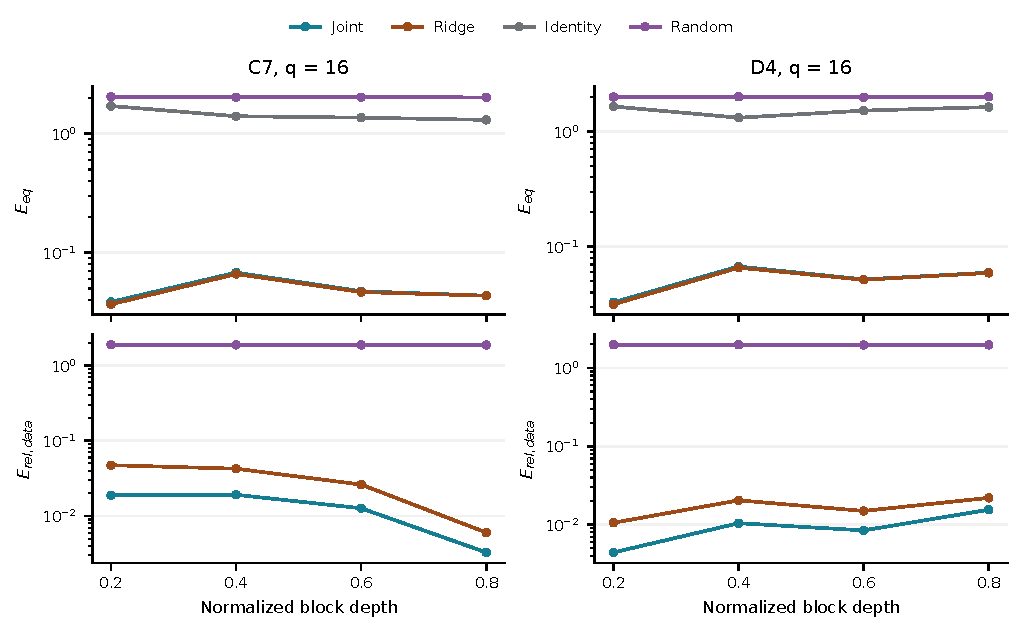
\includegraphics[width=.85\textwidth]{figures/structural_errors.pdf}
\caption{Historical direct prediction and relation consistency across the fixed six-model FULL panel at $q=16$. Joint fitting changes the prediction--consistency tradeoff; the diagnostics do not isolate semantic specificity.}
\label{fig:historical-structural}
\end{figure}
\begin{figure}[t]
\centering
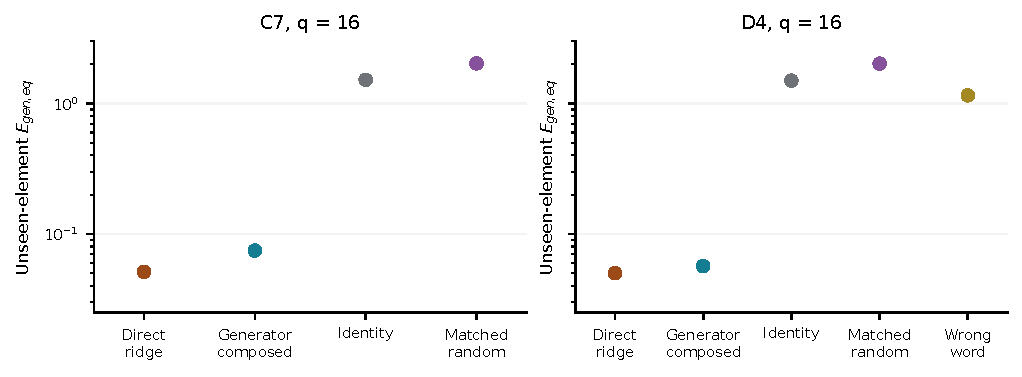
\includegraphics[width=.85\textwidth]{figures/generator_transfer.pdf}
\caption{Generator-only predictions evaluated against transformed held-out activations. Direct element-specific Ridge receives additional supervision. Identity, random generators and wrong words address distinct alternatives. These are the unchanged historical figure values.}
\label{fig:historical-generator}
\end{figure}
Joint relation defects decrease relative to Ridge by $-0.01699$ (recorded 95\% bootstrap interval $[-0.03405,-0.00318]$) for $C_7$ and $-0.00728$ ($[-0.01248,-0.00259]$) for $D_4$. For $D_4$, joint data relation components are $0.01717$ for $r^4$, $0.00876$ for $s^2$, and $0.00320$ for $srs=r^{-1}$. They are approximate relations on activations, not certification of exact ambient representations. In AFS-A, the correct-minus-wrong-word $D_4$ contrast is $-1.097329$ ($[-1.219881,-0.953809]$). All intervals retain the resampling-sensitivity scope of \cref{app:inference}.


The historical FULL joint-minus-random $\Eeq$ contrasts are $-1.9803$ ($[-2.0041,-1.9549]$) for $C_7$ and $-1.9449$ ($[-1.9562,-1.9325]$) for $D_4$. Joint-minus-identity values are $-1.3964$ ($[-1.5882,-1.1982]$) and $-1.4771$ ($[-1.6692,-1.2628]$). These large differences establish useful transformation prediction relative to untrained controls. The more demanding joint-minus-ridge prediction contrasts are slightly positive: $0.001046$ ($[0.000106,0.002285]$) and $0.000864$ ($[0.000149,0.001735]$). Joint-minus-ridge homomorphism differences are $-0.000884$ ($[-0.002083,-0.000018]$) and $-0.000891$ ($[-0.001652,-0.000232]$). These are effects under the historical resampling procedure; their small intervals do not resolve the identification alternatives in \cref{sec:boundaries}.


\begin{table}[h]
\centering
\small
\begin{tabular}{llccc}
\toprule
Group & Estimator & $\Ehom/\Ehomop$ & $\Erel/\Erelop$ & $\Ecomp/\Ecompop$ \\
\midrule
$C_7$ & Joint & 0.00842 / 0.05850 & 0.01348 / 0.09612 & 0.01145 / 0.07879 \\
$C_7$ & Ridge & 0.00930 / 0.06202 & 0.03047 / 0.20903 & 0.01266 / 0.08438 \\
$C_7$ & Random & 1.45937 / 1.03612 & 1.87118 / 1.45048 & 1.98636 / 1.41027 \\
$D_4$ & Joint & 0.00366 / 0.10143 & 0.00971 / 0.17124 & 0.00477 / 0.13149 \\
$D_4$ & Ridge & 0.00455 / 0.11897 & 0.01699 / 0.26283 & 0.00594 / 0.15530 \\
$D_4$ & Random & 1.52346 / 1.08021 & 1.96710 / 1.39203 & 1.98983 / 1.41088 \\
\bottomrule
\end{tabular}
\caption{Recorded primary FULL consistency diagnostics at dimension 16. Data/op pairs deliberately preserve distinct historical metrics: data defects are squared and op defects unsquared; C7 relation aggregands additionally differ. These paired columns should not be read as a comparison on one numerical scale. Homomorphism and composition differ only by excluding identity-containing pairs in the latter.}
\label{tab:full-diagnostics}
\end{table}

\begin{table*}[t]
\centering
\small
\begin{tabular}{lll}
\toprule
Control & Group/metric & Frozen summary \\
\midrule
AFS-B & C7, data homomorphism & 120/120 below reference 2.5th percentile \\
AFS-B & C7, operator homomorphism & 120/120 below reference 2.5th percentile \\
AFS-B & D4, data homomorphism & 120/120 below reference 2.5th percentile \\
AFS-B & D4, operator homomorphism & 120/120 below reference 2.5th percentile \\
AFS-C & C7, state relabel & $-0.577\;[-0.664,\,-0.488]$ \\
AFS-C & C7, target scramble & $-0.596\;[-0.686,\,-0.506]$ \\
AFS-C & D4, state relabel & $-0.765\;[-0.861,\,-0.662]$ \\
AFS-C & D4, target scramble & $-0.729\;[-0.824,\,-0.627]$ \\
\midrule
Global additive & Balanced complete orbit & $\widehat v_g=0$ by permutation cancellation \\
\bottomrule
\end{tabular}
\caption{Registration/correspondence controls and the scope of global additive falsification. AFS-C reports real-minus-scrambled test equivariance error after refitting on perturbed training pairs and scoring against unchanged true held-out targets; negative values favor the real correspondence. Brackets retain the historical bootstrap percentile intervals. AFS-B compares fixed operators with a restricted reference excluding automorphisms; observed and reference registrations are not established as exchangeable, so this is not calibrated semantic-null inference. The global displacement estimator averages complete state orbits and therefore reduces to identity independently of the activations.}
\label{tab:diagnostic-controls}
\end{table*}

AFS-B preserves the fitted matrix family while changing which algebraic element each matrix represents. AFS-C instead changes training correspondence while retaining the activation multiset, refits Ridge and scores it against the true held-out targets. In both groups and both scramble variants, the recorded mean test prediction and data-relation defects increase. The latter are consistency diagnostics on held-out activations, not additional semantic-target accuracy measurements. Prediction error and operator norms are not matched across conditions; moreover, the $C_7$ power-consistency and $D_4$ $srs$ terms normalize by condition-specific fitted outputs. The deterioration therefore does not isolate algebraic fidelity beyond the change in predictive fit. Neither AFS-B nor AFS-C demonstrates that a consistently registered alternative action of comparable learnability would fail.

\subsection{Rank-matched lexical comparison}
\begin{table*}[t]
\centering
\small
\begin{tabular}{lllrrr}
\toprule
Group & Model & Location & $E_{\rm eq}$ & $E_{\rm gen,eq}$ & $E_{\rm rel,data}$ \\
\midrule
C7 & Llama 1B & Embedding & $3.64\!\times\!10^{-6}$ & $5.87\!\times\!10^{-5}$ & $6.37\!\times\!10^{-5}$ \\
C7 & Llama 1B & Internal mean & 0.132327 & 0.198978 & 0.092076 \\
C7 & Qwen 1.5B & Embedding & $2.48\!\times\!10^{-6}$ & $4.25\!\times\!10^{-5}$ & $4.72\!\times\!10^{-5}$ \\
C7 & Qwen 1.5B & Internal mean & 0.171656 & 0.315743 & 0.187296 \\
D4 & Llama 1B & Embedding & $4.97\!\times\!10^{-7}$ & $2.97\!\times\!10^{-6}$ & $3.95\!\times\!10^{-6}$ \\
D4 & Llama 1B & Internal mean & 0.096634 & 0.133246 & 0.051652 \\
D4 & Qwen 1.5B & Embedding & $3.02\!\times\!10^{-7}$ & $1.80\!\times\!10^{-6}$ & $2.39\!\times\!10^{-6}$ \\
D4 & Qwen 1.5B & Internal mean & 0.055191 & 0.059383 & 0.027160 \\
\bottomrule
\end{tabular}
\caption{Rank-matched lexical control using independent Ridge, with generator-only composed predictions for $E_{\rm gen,eq}$. Matching refers to training projected rank, supported by audited input spectra and the recorded PCA procedure rather than direct remeasurement of historical coordinates (\cref{app:dimension-rank-audit}). Both locations use C7 $q=6$ or D4 $q=3$; these are not the FULL $q=16$ estimates. Internal means average four fixed depths. Embedding errors are smaller in every tested model/group; all 150 archived internal-minus-embedding intervals are positive. Repeated templates at the embedding location reuse the same category vectors.}
\label{tab:lexical-control}
\end{table*}

\begin{figure}[h]
\centering
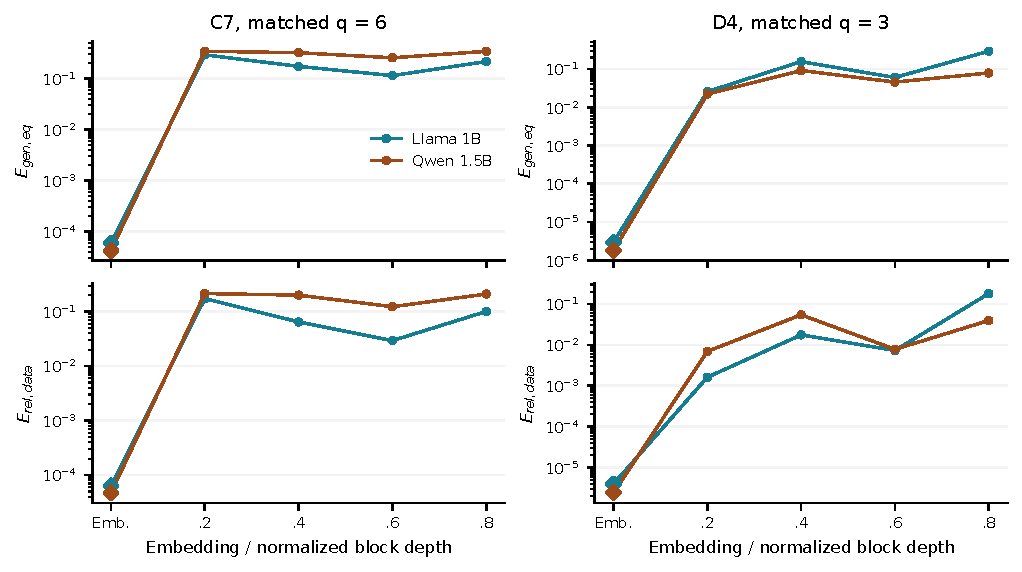
\includegraphics[width=0.76\textwidth]{figures/lexical_internal.pdf}
\caption{AFS-D independent fits matched in training projected rank: $q=6$ for $C_7$, $q=3$ for $D_4$. This two-model comparison is separate from primary FULL at dimension 16. Audited input spectra and the recorded PCA procedure support the training-rank match; historical projected arrays are unavailable for direct checks (\cref{app:dimension-rank-audit}). Lexical near-exactness is compatible with finite-orbit realizability.}
\label{fig:lexical}
\end{figure}
Across the two models and two groups, the internal-minus-embedding contrasts are positive for both prediction and data relation error. This is evidence against internal strengthening in this recorded comparison. It is not evidence that embedding representations encode the uniquely correct semantic action; the full-rank lexical vectors permit every state permutation. Nor does it imply that arbitrary dimensions, models, reading positions, or contextual constructions behave identically.

\subsection{Global additive-field results}
The historical global-field direct errors are additive 1.487859, ridge 0.050149, and joint 0.051104. The additive-minus-ridge contrast is 1.437710 ($[1.400230,1.475673]$), and additive-minus-joint is 1.436755 ($[1.399237,1.474462]$). For repeated C7 generator prediction, the errors are 1.519200, 0.074443, and 0.070297. For the combined D4 paths $r\to s$, $s\to r$, and $s\to r\to s$, they are 1.266128, 0.049265, and 0.047450.

These are the completed experiment's observation-weighted means, not replacements for the FULL or AFS-A primary aggregates. The additive estimator cancels for every action because training covers complete, balanced state orbits. Repeated additive updates therefore cannot track even cyclic motion; for D4, they also cannot distinguish word orders because addition commutes. The reported descriptive order separation is 2.2133 for actual contextual targets, 2.2789 for ridge predictions, and 2.2526 for joint predictions, while the additive prediction has zero separation by construction. The first three are descriptive scores under the recorded normalization, not calibrated accuracies or independent confirmatory tests.

\subsection{Behavioral patching}
\label{app:behavior}
The evaluation prompt appends `` Report the transformed state:'' to a held-out structural prompt. The state remains visible, and the particular transformation is supplied through the selected activation intervention rather than by an explicit textual instruction naming $g$. Let $h$ be the mean state-span hidden vector from this evaluation prompt, $z=(h-\hat{\mu})U_{\mathrm{PCA}}$, and $U_{\mathrm{PCA}}$ the structural training-only PCA basis. The learned replacement is
\[
 h'=h-zU_{\mathrm{PCA}}^\top+(zR_g)U_{\mathrm{PCA}}^\top.
\]
The forward hook replaces every token position overlapping the state string with this replacement vector at the selected transformer block output, then recomputes the remaining network. If a state occupies multiple input tokens, all overlapping positions receive the same replacement derived from the mean; identity uses the original unpatched output. Thus an identity-matrix patch need not equal the unpatched baseline: overwriting distinct token vectors with their mean can itself change the network. The historical run does not contain a matched zero-delta, token-deviation-preserving sham. The one-token continuation counts below do not establish one-token source spans. These implementation details limit interpretation as a natural state substitution.

The source-conditioned additive comparator is trained from structural training prompts in the original hidden dimension:
\[
 v_{g,i}=\frac1{|\mathcal T_{\mathrm{train}}|}\sum_{t\in\mathcal T_{\mathrm{train}}}
 (h_{g(i),t}-h_{i,t}),\qquad h'=h+v_{g,i}.
\]
It uses known source-state identity and one vector per element/source pair, so it is more flexible than one source-shared linear operator. Its displacement also acts in the original hidden space, whereas the learned operator changes only the PCA component. The comparison therefore differs in source information, retained parameters and allowed edit subspace. It is an informative stronger comparator because it avoids orbit-averaging cancellation, but it is not a parameter- or subspace-matched test of steering optimality. In the recorded D4 relation rows the additive edit is indexed by the requested target element, so the true word, its direct reference and the wrong-word control receive the same endpoint-conditioned displacement; their equality for this comparator is built into the construction and does not test its composition order.

The target-token score uses the first token of the context-sensitive continuation `` \{target state\}''. Target logit change and target probability change subtract the unpatched prompt's values. The margin is target minus original-state first-token logit, and top-1 success requires the predicted vocabulary argmax to be that target token. The implementation records a full target-sequence log probability only for one-token continuations and would omit multi-token cases for that metric. All archived evaluated continuations contain one token. The scored top-1 outcome therefore concerns that continuation token; this experiment does not test general multi-token answer accuracy.

\begin{table*}[t]
\centering
\small
\begin{tabular}{llll}
\toprule
Group & Metric & Learned minus identity [95\% interval] & Learned minus additive [95\% interval] \\
\midrule
C7 & Target logit & $1.129\;[0.791,\,1.400]$ & $-0.105\;[-0.227,\,-0.014]$ \\
C7 & Top-1 (pp) & $1.743\;[-0.215,\,3.945]$ & $-0.261\;[-1.065,\,0.056]$ \\
D4 & Target logit & $2.406\;[1.932,\,2.833]$ & $-0.007\;[-0.030,\,0.012]$ \\
D4 & Top-1 (pp) & $9.019\;[3.186,\,15.339]$ & $-0.043\;[-0.503,\,0.434]$ \\
\midrule
\multicolumn{4}{l}{D4 correct-minus-wrong final-logit distance: $-0.0422\;[-0.0543,\,-0.0298]$.} \\
\bottomrule
\end{tabular}
\caption{Frozen behavioral contrasts from externally composed activation edits. Additive denotes the training-only source- and transformation-conditioned comparator, distinct from the global additive field. Positive logit/accuracy differences favor the learned edit; the D4 distance contrast is lower for the correct word. Top-1 measures the scored continuation token; all archived continuation counts are one. Recorded 95\% bootstrap percentile intervals preserve the original nested procedure; they describe fixed-panel resampling sensitivity, not calibrated population coverage (\cref{app:inference}).}
\label{tab:causal-main}
\end{table*}

\begin{figure}[h]
\centering
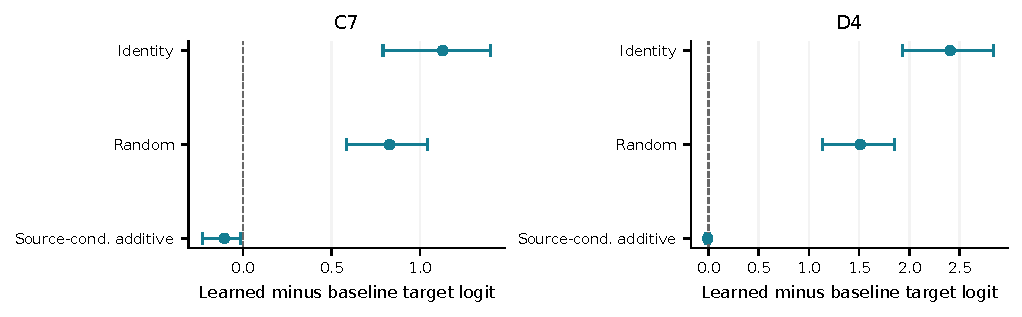
\includegraphics[width=0.76\textwidth]{figures/causal_additive.pdf}
\caption{Learned-minus-source-conditioned-additive target-logit effects. Negative differences favor the stronger additive comparator for that outcome. Directional behavioral effects do not demonstrate causal necessity of a recovered matrix family.}
\label{fig:causal}
\end{figure}
For C7, powers $r^1,\ldots,r^6$ are transformation interventions; $r^7$ is a separate cycle diagnostic. D4 tests $r,s,r^2,r^3$, identity-recovery words $r^4,s^2$, and the relation word $srs$ against a direct $r^{-1}$ intervention. The matched-length wrong word is $rsr$. For final next-token logit vectors $L$, the relation distance is
\[
 d(w,r^{-1})=\frac{\norm{L^{(w)}-L^{(r^{-1})}}_2}{\max(\norm{L^{(r^{-1})}}_2,\epsilon)}.
\]
The historical correct-minus-wrong distance difference is $-0.04220$ ($[-0.05426,-0.02981]$). Both words are evaluated relative to the same direct learned reference; this is an order-sensitive downstream consistency diagnostic, not comparison with a unique ground-truth causal mechanism. The C7 learned-minus-identity target-logit gain is 1.129 ($[0.791,1.400]$), and learned-minus-random is 0.828 ($[0.585,1.041]$). C7 top-1 evidence is weak. Learned-minus-additive target-logit intervals favor the additive baseline in C7 and include zero in D4. Together these observations support behavioral relevance with substantial causal ambiguity. Calendar interventions and competing group-operation mechanisms already demonstrate why an editable representation need not identify native computation \citep{engels2025notall,wu2025unified,feucht2026arithmetic}; the same caution applies to the externally composed edits here.

\FloatBarrier
\subsection{Cross-model compatibility}
Nine fixed pairs comprise all three within-Llama pairs, all three within-Qwen pairs, and size-matched cross-family pairs (1B/1.5B, 3B/3B, 8B/7B). For systems $R_A,R_B$, a row-coordinate map $T$ is assessed through
\[
 R_A(g)T\approx TR_B(g).
\]
The implementation writes $T=P^\top$, stacks the linear constraints $PR_A(g)^\top-R_B(g)^\top P$, takes the smallest right-singular-vector solution, and normalizes $\norm{P}_F=1$. It does not require $P$ to be invertible, well-conditioned, orthogonal, or high effective rank. The normalized score is
\[
 \frac{\mathbb{E}_g\norm{PR_A(g)^\top-R_B(g)^\top P}_F^2}
 {\mathbb{E}_g\norm{R_B(g)^\top P}_F^2+10^{-12}}.
\]
Comparators include an orthogonal Procrustes map estimated from registered activation correspondence, random orthogonal maps, and shuffled group labels. The Procrustes map is fitted on the reported test-template activation pairs and optimizes activation reconstruction, while the intertwiner optimizes commutation using the same group elements later scored. This is a descriptive comparison of two fitting criteria, not predictive transport to unseen paired activations or held-out elements. A low-rank common subspace may suffice. The shuffled-label control keeps the map fitted under true labels rather than refitting after shuffling; it tests sensitivity of that map to registration, not the best achievable fit under each alternative. Shuffled-label controls can also be near-degenerate.

Unlike implementation-family comparisons based on causal abstractions and Congruity \citep{sun2026tracking}, this experiment neither samples behavior-preserving implementations nor estimates their abstraction-dependent distance. The recorded fitted-minus-Procrustes residual differences range approximately from $-0.065$ to $-0.168$ over the registered strata, with historical intervals below zero. This establishes existence of lower-residual fitted commutation maps than the chosen geometry alignment on these elements, not cross-model representation equivalence. The recorded Spearman association with conventional linear CKA is $-0.014$ with interval $[-0.300,0.287]$, leaving that relationship unresolved.

\subsection{Completed controls and remaining identification scope}
The characterization supplies state-centroid, residual and input-only field comparisons under its own sampling and normalization contract. The returned extension additionally completes full-data compact nonlinear predictors, coherent alternative registration, direct context-difference fits and peer adaptations (\cref{app:reproduction}). Their descriptive results are now part of the evidence; they do not retroactively repair a historical comparison's information or intervention mismatch.

The remaining gaps concern stronger claims than the fixed-panel predictive account retained here: algebraic evidence beyond prediction would require a direct-error- and operator-norm-matched comparison; cross-vocabulary generalization would require genuinely new lexical realizations and independently authored context families; native causal use would require competent-task counterfactual evidence. Native confirmation remains blocked despite completed secondary adaptations. None of those stronger claims is inferred from the present comparisons. Future method selection on the inspected holdout would be exploratory and would need fresh evaluation before confirmation. A same-order wrong-group comparison also requires a feasible matched action: no four-state permutation has order eight, so $C_8$ cannot act faithfully on the four corners. An impossible alternative is not an error-matched semantic reference.

\section{Study 2: Coordinate Banks and Original Characterization}
\label{app:characterization}
The original coordinate characterization was specified after excluded development comparisons. It completed 72 model/readout/domain cells, 120 structural split records and 48 $C_7/D_4$ field-comparison cells. The results below are reviewed descriptive aggregates. Original source flags and failed decisions remain unchanged in the release archive. Because these evaluation outputs have been inspected, they cannot serve as untouched data for later method selection.

\paragraph{Data and information conditions.}
The same six pinned base models and four readouts use training-only $q=16$ coordinates, with BF16 model extraction and F64 coordinate analysis. New extraction comprises 41,728 rows per model: 896 $C_7$, 512 $D_4$ and 40,320 $S_3$ rows, including separately charged support. The C7/D4 state vocabularies are seen in construction. S3 also retains its six abstract assignment states, but its new-entity and joint strata hold out entity names/triples. Unseen-composite supervision concerns actions, not new C7/D4 states or independently authored grammar roots. Coordinate fields receive source coordinates and the requested action. The separate decoded-centroid benchmark has training state labels and the known action table, but decodes the source at evaluation. In contrast, the legacy prediction contrasts in \cref{tab:characterization-intervals} select oracle-source category/retention controls (and an input-metadata potential for S3) on validation; they are not the decoded-source benchmark.

\paragraph{Losses and aggregation.}
The characterization normalizes squared errors by common training-only energy scales; the historical $D$ in \cref{eq:D} averages per-row target-normalized errors. Values across the two studies are therefore not interchangeable. Writing $\bar z_{\rm tr}$ for the training mean, prediction uses $E_z=\mathbb{E}_{\rm tr}\norm{z-\bar z_{\rm tr}}_2^2$. For two paraphrases ordered by their registered identifiers, set $u=z_{p_0}-z_{p_1}$; transport uses $E_u=\mathbb{E}_{\rm tr}\norm{u}_2^2$, without recentering. The row losses are $\norm{\widehat z_g-z_{g(i)}}_2^2/E_z$ and $\norm{\widehat u_g-u_{g(i)}}_2^2/E_u$. Validation and evaluation retain only changed-state pairs $g(i)\ne i$. All-element fitting still uses all training pairs, including identity/fixed points; generator fitting and selection use only primitives. Historical nonidentity-action averages can include D4 fixed points. Prediction and transport thus differ in denominator as well as target. These original coordinate summaries pool changed-state pairs; the later equal-action aggregation is explicitly distinguished in \cref{app:aggregation-contract}. Models and readouts form a fixed panel, averaged within family/entity units. The resampling units are $64\times1$ for $C_7/D_4$, $64\times16$ for jointly new $S_3$ contexts/entities, $64\times24$ for new contexts, and $48\times16$ for new entities. Independently resampled family/entity indices give the crossed $S_3$ sensitivities. No new superiority, equivalence or multiplicity-controlled decision is made.
\begin{table}[htbp]\centering\small
\begin{tabular}{llrrr}\toprule
Domain / split & Endpoint & Baseline minus linear & Lower & Upper \\
\midrule
$C_7$, new context & prediction & -0.002887 & -0.003290 & -0.002495 \\
$C_7$, new context & context & 0.011485 & 0.009997 & 0.013087 \\
$D_4$, new context & prediction & 0.019612 & 0.014730 & 0.025945 \\
$D_4$, new context & context & 0.060918 & 0.049883 & 0.072920 \\
$S_3$, context & prediction & -0.000487 & -0.000791 & -0.000249 \\
$S_3$, context & context & 0.000177 & 0.000010 & 0.000348 \\
$S_3$, entity & prediction & 0.000673 & 0.000443 & 0.000927 \\
$S_3$, entity & context & 0.000739 & 0.000542 & 0.000978 \\
$S_3$, joint & prediction & 0.000460 & 0.000262 & 0.000673 \\
$S_3$, joint & context & 0.000154 & -0.000017 & 0.000338 \\
\bottomrule\end{tabular}
\caption{All ten original characterization contrasts with frozen 95\% percentile sensitivity intervals (10,000 draws, seed 314159). Positive favors linear. Prediction uses oracle-source category/retention controls, plus the $S_3$ input-metadata potential, selected on validation; context uses scalar retention. Prediction and context have different training-energy denominators. Fixed-panel sensitivities do not certify significance, equivalence, coverage or an old power gate.}
\label{tab:characterization-intervals}\end{table}


\paragraph{Prediction and compact category controls.}
All-element direct ridge versus full-kernel means are $0.014900/0.004626$ for $C_7$ and $0.041349/0.020916$ for $D_4$. A training-centroid displacement predictor uses
\[
 \widehat z_g=z+\mu_{g(\widehat i(z))}-\mu_{\widehat i(z)},
\]
where $\widehat i$ is the nearest training centroid. Source decoding is perfect in all $C_7/D_4$ field conditions. C7's error is $0.012013$, better than ridge on average but in only 9/24 individual conditions; D4's $0.062349$ is worse on average and improves only 2/24. Centroids occupy 112 and 64 floating-point coordinates, respectively, plus the exact integer action table and decoding logic. This is a strong cheap control under additional construction labels, not a strict match to label-free field information. Evaluating a known composite label after one source decode is also distinct from repeated primitive evaluation with re-decoding at each intermediate output; the former cannot certify the latter.

\begin{figure}[t]\centering
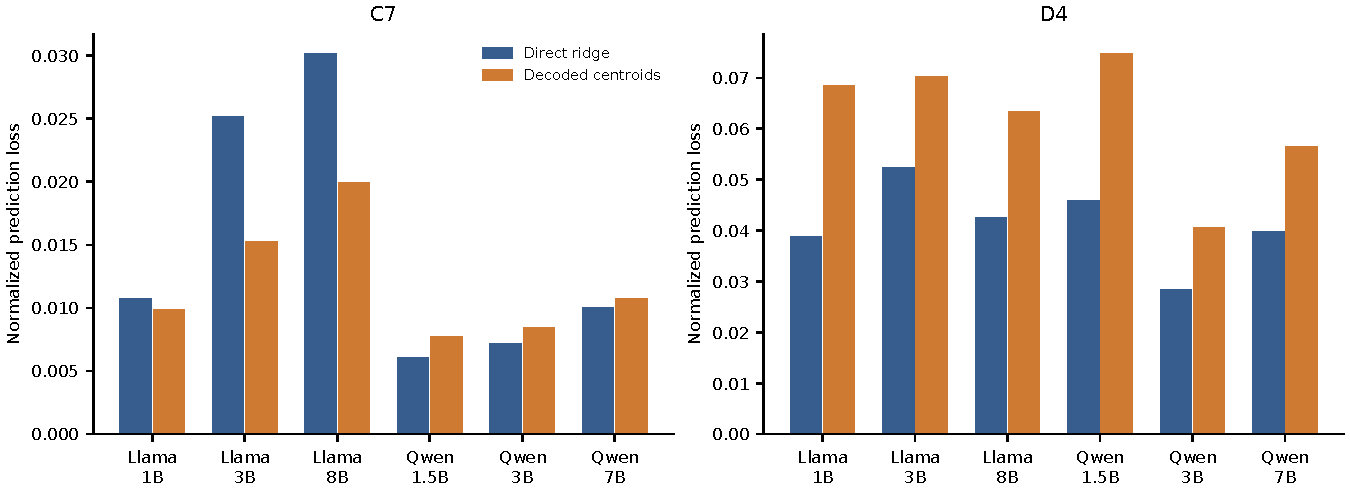
\includegraphics[width=.95\textwidth]{figures/characterization_baselines.pdf}
\caption{All-element prediction: four-readout means for six fixed models. The C7 mean comparison favors decoded centroids in the three Llama models and ridge in the three Qwen models; D4 favors ridge on all six model means. These identities are not independent draws from model lineages. The category comparator has training labels and a known action table. Common PCA and runtime costs are excluded from incremental predictor coordinates.}
\label{fig:characterization-baselines}\end{figure}

\paragraph{What the storage curve measures.}
Primitive-only full fields use 21,504 versus 256 retained coordinates for C7 and 18,432 versus 512 for D4 (84 and 36 times). At the small prescribed budgets they use 256 versus 256 and 480 versus 512. Thus D4 is near-budget, not exactly equal. Farthest-first support selection sees all construction source coordinates but retains only $K$ paired displacements; linear regression compresses all construction target pairs into its coefficients. This original comparison did not fit a compressed nonlinear estimator to all target pairs. The completed RFF/Nystr\"om extension in \cref{app:reproduction} now makes that comparison at explicit parameter budgets; its changed-state/identity handling and selection contract are kept separate from these original values. All 48 full primitive bandwidth selections hit the smallest frozen candidate, $0.125$; some reduced-support selections use $0.25$. These facts bound the comparison and motivate a future development-only grid extension, not retrospective test tuning.

All-element stored ridge maps include an avoidable identity matrix: counts are 1792/2048 for C7/D4, or 1536/1792 after deterministic identity handling. Their $K=14$ fields store 1792/2016, or 1568/1792 after removing zero identity-displacement arrays. C7's original nominal match becomes slightly above-budget after pruning. The common PCA center/basis costs $d(q+1)$ stored float64 coordinates in this export. Training memory, model weights, group tables, centroids, biases, normalization, temporary copies and actual precision must be counted separately for a deployment claim. Retained-coordinate counts are neither total RAM nor statistical capacity.

\paragraph{S3 and context limitations.}
Joint S3 identity prediction loss is $0.018939$, compared with ridge $0.018642$; a small absolute loss is not by itself strong action recovery. The joint context-difference contrast spans zero, and the remaining effects are small relative to the original $0.01$ practical margin. Support displacement reduces prediction loss to $0.015282$ jointly and $0.017580$ on new entities using four extra contexts per entity/state; it is not zero-shot operator superiority. Potential controls were selected in 10/24 conditions (30 split records). Their neural optimization has not been independently replayed. The analytic context fit is separate from that potential. No S3 coordinate-kernel, native intervention or cross-model comparison was added to this original characterization. The subsequent context-predictor and secondary extensions are separately identified in \cref{app:reproduction}.

\paragraph{Audit and provenance boundary.}
The returned archive's checksum, 490-member identity, source/configuration pins, model/readout grid, full metadata banks, exported geometry and 56 frozen intervals were verified. New independent NumPy refits and broader analytic replay reproduced supported coordinate calculations to numerical precision. Historical S3 development selection retains 9,216 reserved cross-block rows per model; exact identities and fitting/scoring masks were checked rather than accepting arbitrary reserved data. The public workflow now validates this historical bank explicitly. Input-feature preprocessing can enumerate nontraining source metadata while assigning zero fitting weight outside training; this is not fitting held-out targets.

The original characterization and its later computational replay are not two independent samples. Compact exports cannot prove original forwards, raw-to-PCA fits, omitted repeated embedding equality or universal prior-access history. Neural Joint/potential refits remain conditional. These limits are recorded with original archive/source hashes and derivative identities in the accompanying release.

\section{Study 2: Predictor, Transport and Secondary Comparisons}
\label{app:reproduction}
The predictor and transport comparisons reuse the inspected coordinate construction and retain all model/readout conditions. Computational reproduction checks the earlier calculations; it does not supply an independent sample or convert the unsuccessful native protocol into a causal result. The tables are reviewed descriptive derivatives. Original source identities, failure records and eligibility flags remain unchanged in the accompanying archive.

% Generated by scripts/build_identification_table.py; see identification_summary.source.json.
\begin{table*}[t]
\centering\small
\setlength{\tabcolsep}{4pt}
\renewcommand{\arraystretch}{1.10}
\begin{tabular}{@{}p{.16\textwidth}p{.40\textwidth}p{.40\textwidth}@{}}
\toprule
Test and endpoint & Recorded observation ($C_7$ / $D_4$) & Supported conclusion and remaining alternative \\
\midrule
Independent fits\newline (FULL, $D$) & Ridge: 0.04830 / 0.05200. & Shared linear maps predict activations in held-out templates; stable category coding remains compatible. \\
\addlinespace[3pt]
Generator transfer\newline (AFS-A, $D$) & Composed: 0.074443 / 0.056558. \newline Direct: 0.051124 / 0.050032. & Transfer to five excluded action elements; state labels remain seen. Direct fits receive additional element supervision. \\
\addlinespace[3pt]
Context differences\newline (replay transport) & Coordinate fit: 0.047137 / 0.132304. \newline Direct fit: 0.034260 / 0.116386. \newline Coherent fit: 0.034465 / 0.117165. & Direct fitting helps; a coherent alternative has close means. Targets and masks are registration-specific; closeness is not equivalence. \\
\addlinespace[3pt]
Compact nonlinear\newline (replay prediction) & First tested budget with lower mean than ridge, in both groups:\newline Nystr\"om $2\times$; RFF $4\times$. & Predictor ranking depends on storage. Parameter bytes do not match statistical capacity or runtime. \\
\addlinespace[3pt]
Category control\newline (replay prediction) & Centroid: 0.012013 / 0.063821. \newline Ridge: 0.014897 / 0.041919. \newline Centroid lower in 9/24 / 2/24 cells. & Category coding is competitive for the C7 mean, not most cells; centroids receive extra training labels and the action table. \\
\addlinespace[3pt]
Restricted registration\newline (AFS-B) & 120/120 cells in each group, separately for data and operator defects, below the reference 2.5th percentile. & Separation from invalid registrations; the restricted ensemble is not a calibrated semantic null. \\
\bottomrule
\end{tabular}
\caption{Evidence and identification boundaries. Paired numbers are $C_7$ / $D_4$ (corners); smaller losses are better. Rows concern different experiments, not one matched comparison or independent confirmations. Historical $D$ averages per-row target-normalized squared errors; replay prediction and context transport use distinct training-energy denominators $E_z$ and $E_u$. Compare losses only within the stated study and endpoint. Replay means cover 24 fixed model/readout cells per group. Budget crossovers are descriptive across the full recorded grid, not a test-selected deployment policy. D4 fixed-point identities, and hence scored rows, can differ across registrations. Statistical scope is defined in Section~\ref{sec:setup}.}
\label{tab:identification-summary}
\end{table*}


\subsection{Completed scope and preserved stopping decisions}
\begin{table}[t]\centering\small
\caption{Completed computations and scientific stopping decisions. ``Complete'' concerns the named computation; scientific eligibility is separately stated. No absent confirmation result is imputed from a completed secondary branch.}
\label{tab:reproduction-status}
\begin{tabular}{p{.31\textwidth}p{.61\textwidth}}\toprule
Component & Recorded outcome and interpretation \\\midrule
Structural recovery and pilot & Complete; archived computations agree with the previous frozen tables. \\
AFS A/B/C and additive extensions & Complete under their historical definitions; pass labels do not exclude all category/context explanations. \\
Original $q=16$ embedding AFS-D & Infeasible: centered lexical training rank is six in the failing weekday cell. Original failed unit retained. \\
Separate rank-aware AFS-D & Complete at $q=6$ for $C_7$ and $q=3$ for $D_4$; embedding-dominant diagnostic, not a replacement $q=16$ pass. \\
Original synthetic calibration & Stopped: recorded Y4 sensitivities $0.870$ ($C_7$) and $0.825$ ($D_4$) are below $0.90$. \\
Revised BF16/F64 calibration & Complete; passed its specified synthetic-generator criteria. \\
Characterization / compact--context & Complete; 72 coordinate cells / 240 component--registration jobs. Descriptive analyses of inspected designs. \\
Structural power & Limited precision; no selected family count or overall powered-confirmation claim. Separate $S_3$ planning target met. \\
Pilot / native preparation & Stopped: first $m_0.C_7$ clean accuracies are $0.0625$ development and $0.15625$ transfer, below $0.80$. \\
Structural / native confirmation & Blocked by their scientific dependencies; no confirmatory outcomes. \\
Peer, cross-model, product, interface & Complete as separate secondary diagnostics; their scopes are detailed below. \\
\bottomrule\end{tabular}
\end{table}

The native stop concerns the registered program task and endpoint. Shorter or differently prompted development diagnostics cannot substitute for its gate. Likewise, a synthetic calibration pass assesses the specified decision procedure under simulated regimes; it does not certify a native mechanism. The structural power assessment reports limited precision and supports no powered-confirmation claim. A separate $S_3$ planning calculation selects 64 families and 16 orbits, without overriding the blocked overall confirmation.

\subsection{Compact nonlinear predictors and coherent registration}
The compact extension reads the completed $q=16$ coordinate banks with unchanged training, validation and test roles. It includes independent linear and affine ridge, decoded-centroid displacement, limited-support Gaussian fields, random Fourier feature residual regression, and Nystr\"om residual regression. The last two fit all construction target pairs at each budget. Training-source landmarks, feature parameters, normalizers, coefficients, biases and numeric lookup tables are charged to incremental float64/int64 parameter storage. Shared PCA, model weights, temporary arrays and Python/runtime overhead are excluded. Logical parameter bytes are not compressed file size, total RAM or a statistical-capacity equivalence.

\begin{table}[htbp]\centering\small
\begin{tabular}{lrr}\toprule
Method & $C_7$ & $D_4$ (corners) \\
\midrule
Ridge & 0.01490 & 0.04192 \\
Decoded centroid & 0.01201 & 0.06382 \\
Limited support, $1\times$ & 0.66133 & 0.49167 \\
RFF, $1\times$ & 0.30033 & 0.21265 \\
Nystr\"om, $1\times$ & 0.08292 & 0.04942 \\
\bottomrule\end{tabular}
\caption{All-element changed-state prediction in the reviewed replay: equal action then equal cell means over 24 fixed model/readout cells per group; lower is better. $1\times$ denotes nominal incremental storage relative to ridge, not equal capacity or total RAM. Centroids additionally use construction labels and an action table. All budget and registration results are retained in the release.}
\label{tab:reproduction-compact}\end{table}

\begin{table}[htbp]\centering\small
\begin{tabular}{llrrrrr}\toprule
Group & Estimator & $0.5\times$ & $1\times$ & $2\times$ & $4\times$ & $8\times$ \\
\midrule
$C_7$ & Limited support & 0.76776 & 0.66133 & 0.65234 & 0.64495 & 0.64310 \\
$C_7$ & RFF & 0.93529 & 0.30033 & 0.06631 & 0.01174 & 0.00708 \\
$C_7$ & Nystr\"om & 0.49296 & 0.08292 & 0.01243 & 0.00845 & 0.00612 \\
$D_4$ & Limited support & 0.52597 & 0.49167 & 0.48148 & 0.47483 & 0.47389 \\
$D_4$ & RFF & 0.63453 & 0.21265 & 0.06644 & 0.02778 & 0.02229 \\
$D_4$ & Nystr\"om & 0.17035 & 0.04942 & 0.03153 & 0.02333 & 0.01960 \\
\bottomrule\end{tabular}
\caption{All five declared nominal budgets for the all-element semantic track, equal action then equal cell means over 24 cells. This table does not choose a budget on the inspected test set. Generator-only and coherent-action results remain separate in the machine-readable release.}
\label{tab:reproduction-budgets}\end{table}

Fixed budgets are $0.5,1,2,4,8$ times the identity-pruned linear reference (\cref{tab:reproduction-budgets}). The all-element and primitive-only tracks have different supervision. Primitive composition repeatedly applies each predictor to its own output, including repeated source decoding for centroids. Infeasible budget conditions and invalid predictions remain explicit. Validation selects the prescribed candidates without using test targets; all budgets and all cells remain in the released summaries. \Cref{tab:reproduction-compact} reports the fixed unit-budget all-element comparison rather than a test-selected operating point. The complete curve shows that Nystr\"om improves mean error over ridge at $2\times$ and RFF at $4\times$ storage in both groups. This descriptive operating-point comparison is distinct from a validation-selected deployment policy; selecting a budget retrospectively on these test means would require new evaluation.

The decoded-centroid control receives construction state labels and an exact group-action table, beyond source-coordinate/action access. Its unit-budget all-element means are $0.012013$ and $0.063821$ for $C_7/D_4$, versus ridge $0.014897$ and $0.041919$. With primitive-only fitting, generator-composed means over all nonidentity actions are $0.012013/0.063821$ for centroids and $0.021114/0.045896$ for ridge. The unit-budget Nystr\"om means on that track are $3.643199/0.087822$; a good direct predictor need not yield stable repeated composition. This all-action aggregate includes the fitted generators and must not be described as an unseen-element-only endpoint. These are descriptive means, without a claim that the selected nonlinear designs exhaust the alternative class. They must not silently replace the original characterization's related but distinct fitting/identity-handling tables.

\paragraph{Why the D4 means differ between the two coordinate analyses.}
\label{app:aggregation-contract}
The original characterization in \cref{app:characterization} pools changed source/action pairs before averaging, whereas the compact extension first averages the changed-state losses within each action and then gives actions equal weight. D4 elements can move different numbers of corners, so pooled-pair and equal-action weighting differ. Every nonidentity C7 action moves all seven weekdays, so this particular weighting difference vanishes there. Ridge fitting and identity handling also differ between the protocols. Thus the characterization's D4 centroid/ridge means $0.062349/0.041349$ and the compact extension's $0.063821/0.041919$ are separate recorded endpoints, not interchangeable estimates of an identical aggregate. The main table uses the compact endpoint; neither original result is overwritten. The weighting explanation follows the saved analysis code and does not claim a new numerical decomposition of the difference.

Every action is also conjugated by the fixed state swap $(0,1)$ to define a coherent alternative registration. The alternative preserves group laws and fixed-point counts and uses the same supervision format and fitting procedure, applied to its own consistent target correspondence. All-element ridge means are $0.017503/0.041871$ for this registration, versus semantic $0.014897/0.041919$. Both use the same underlying source bank and abstract action labels, but targets and changed-state evaluation masks are registration-specific. The $D_4$ scored rows can differ because conjugacy preserves fixed-point counts without fixing their identities; this is not an identical-row, identical-target comparison. One conjugate reference is neither an exhaustive comparison with all finite actions nor an exchangeable randomization test. A validation-only comparability ledger retains both matched and unmatched conditions under the fixed 1.25 factor for error and output squared norm, plus linear coefficient norm where available. This does not match nonlinear Jacobian norms.

\begin{table}[htbp]\centering\small
\begin{tabular}{lrr}\toprule
Method & $C_7$ & $D_4$ (corners) \\
\midrule
Ridge & 0.023180 & 0.048802 \\
Decoded centroid & 0.012814 & 0.066672 \\
Limited support, $1\times$ & 1.547945 & 0.899571 \\
RFF, $1\times$ & 3.040965 & 0.390158 \\
Nystr\"om, $1\times$ & 4.304052 & 0.095135 \\
\bottomrule\end{tabular}
\caption{Generator-only fitting evaluated solely on the five excluded nonidentity elements in each group. Equal action means precede equal means over 24 cells. The unit storage budget now refers to generator matrices. These numbers are distinct from the all-nonidentity evaluation, which includes fitted generators. No new model or predictor was fitted for this aggregation.}
\label{tab:reproduction-unseen}\end{table}

The separate excluded-element endpoint in \cref{tab:reproduction-unseen} removes the fitted generators before averaging. It is computed from the original saved per-action records, with no predictor refitting.

\subsection{Context-difference transport}
\begin{table}[htbp]\centering\small
\begin{tabular}{lrrr}\toprule
Method & $C_7$ & $D_4$ (corners) & $S_3$ (joint) \\
\midrule
Identity & 0.045755 & 0.181386 & 0.016444 \\
Coordinate-fitted operator & 0.047137 & 0.132304 & 0.016298 \\
Context-fitted linear & 0.034260 & 0.116386 & 0.016290 \\
Oracle category retention & 0.043825 & 0.166675 & 0.016313 \\
Context-fitted, coherent action & 0.034465 & 0.117165 & 0.016291 \\
\bottomrule\end{tabular}
\caption{Context-difference transport on 24 fixed cells per stratum. Coherent swap01 defines a consistently relabeled alternative action; it is not an exchangeable semantic null. Each registration uses its own targets and changed-state mask; retained D4 pairs need not coincide. All predictors within one registration share its scoring rows. The context loss uses its own training-energy normalization, not the coordinate-prediction denominator.}
\label{tab:reproduction-context}\end{table}

For registered paired paraphrases, the source is $u_i=z_{p_0,i}-z_{p_1,i}$ and the target is $u_{g(i)}$. The uncentered training difference energy supplies a common denominator for these comparisons; it differs from coordinate prediction energy and historical per-row normalization. The extension compares identity, per-action scalar retention, coordinate-fitted operators, directly fitted linear difference maps, full-data RFF/Nystr\"om difference regressors, and category-retention controls. The decoded-category arm additionally receives the paired source center; the oracle arm additionally receives the true category. These information advantages remain labeled. Within each registration, the compared predictors share targets and the changed-state mask. Across registrations, targets differ and retained $D_4$ pairs need not coincide. $S_3$ new-context, new-entity and joint strata are separate; reserved/support rows do not enter primary fitting or selection.

To see the scope of this endpoint, write a balanced complete bank as $z_{c,s}=\mu+a_s+b_c+w_{c,s}$, where $\mu$ is the grand mean, $a_s$ and $b_c$ are the centered state and context marginal means, and $w_{c,s}$ is the remaining interaction. Then
\[
 z_{c,s}-z_{c',s}=b_c-b_{c'}+w_{c,s}-w_{c',s}.
\]
The state main effect cancels, but the context main effect remains. Predicting these differences therefore does not isolate the interaction term. Moreover, a nonlinear difference predictor need not be induced by an action $F_g$ on the original coordinates: $F_g(z)-F_g(z')$ need not depend only on $z-z'$. The reported comparison concerns paired context-change prediction.

Dedicated linear difference fitting improves the mean $C_7/D_4$ transport error relative to applying coordinate operators to the differences. The fixed coherent registration yields $0.034465$, $0.117165$ and $0.016291$ for $C_7$, $D_4$ and jointly new $S_3$, close to the semantic means in the table. These context scores also use each registration's own changed-state mask, including potentially different D4 rows. Thus the result supports a distinction between fitting objectives, while leaving semantic specificity unresolved. The $S_3$ joint difference from identity is much smaller than the inherited $0.01$ practical margin; no new power or equivalence decision is assigned from these descriptive means.

\subsection{Constructively trained interfaces}
\begin{table}[htbp]\centering\small
\begin{tabular}{lrrrr}\toprule
Objective & $C_7$ loss & $D_4$ loss & $S_3$ joint loss & $S_3$ joint acc. \\
\midrule
Reconstruction & 0.212166 & 0.244488 & 0.410680 & 0.1657 \\
Orbit augmentation & 0.212144 & 0.244781 & 0.410358 & 0.1659 \\
Equivariance & 0.229303 & 0.254190 & 0.401808 & 0.1671 \\
Group regularization & 0.227646 & 0.253783 & 0.401694 & 0.1671 \\
\bottomrule\end{tabular}
\caption{Validation-selected supervised interfaces: 72 model/readout/seed cells per objective and domain, 500 steps per candidate. The loss is normalized full-hidden target-prediction error; it is not the compact-coordinate endpoint. State classification is an interface-head score, not language-model answer accuracy. Seed replicates are not independent datasets.}
\label{tab:reproduction-interface}\end{table}

The interface extension trains supervised rank-16 encoder/decoder/operator systems on the high-dimensional construction activations. It compares reconstruction, complete-orbit augmentation, equivariance consistency and group regularization. There are 1,728 candidate parameter checkpoints, 500 training steps each, with technical seeds 101, 303 and 909; validation selects 864 arm/seed/cell fits. Each domain's table averages 24 model/readout cells and three seeds. All saved candidates, including unselected regularization weights, remain available.

Adding group regularization does not improve mean full-hidden target prediction over reconstruction for $C_7$ or $D_4$, despite nearly perfect transported-state classification. For $S_3$, the modest prediction improvement accompanies classification near $1/6$ on new entities and joint strata; new-context classification is also weak. This is a constructed supervised interface, not evidence that the unchanged language model uses the learned operators. The high-dimensional training-energy-normalized loss is distinct from the compact-coordinate metric. Equal step counts do not establish equal information, capacity or total computation.

\subsection{Peer adaptations and cross-model/product diagnostics}
\begin{table}[htbp]\centering\small
\begin{tabular}{llrr}\toprule
Task & Method & Error & Conditions \\
\midrule
Word & Procrustes & 3.10155 & 60 \\
Word & Ridge affine & 0.42475 & 60 \\
Word & Hu Eq.~12 (source displacement observed) & 0.52642 & 60 \\
Structural & Procrustes & 7.43045 & 48 \\
Structural & Ridge affine & 0.27236 & 48 \\
Structural & Constrained intertwiner & 0.99194 & 48 \\
$C_4\times C_4$ & primary operator & 0.06035 & 24 \\
$C_4\times C_4$ & joint & 0.07267 & 24 \\
$C_4\times C_4$ & local displacement & 0.00539 & 24 \\
\bottomrule\end{tabular}
\caption{Secondary fixed-panel summaries. Word and structural transport use row-normalized errors; the product endpoint has its own target-energy normalization. Values across tasks are not directly comparable. The Hu adaptation receives source-model test displacements. These are implemented adaptations, not certified peer-author reproductions.}
\label{tab:reproduction-secondary}\end{table}

The peer factorial branch fits conditional-mean/ANOVA tables on construction grids. It retains 76,800 unique recipient/condition scores: 15,360 validation and 61,440 test scores, covering two base models, $C_7$ and the free-eight-state $D_4$ task. Eight conditions combine state/operation/joint edits with full-hidden or matched-subspace support, a three-way ablation and a zero-delta sham. This is an Arora-inspired task adaptation, not verified execution of the authors' code. Zero-delta test generation accuracy is only $22.10\%/1.03\%$ for Llama $C_7/D_4$ and $19.59\%/15.63\%$ for Qwen. The branch therefore supplies diagnostic measurements under poor native competence, not a competent-task causal efficacy certification. Different-target edit and sham accuracies cannot be subtracted as if they measured an identical answer endpoint.

The Engels/Wurgaft anchors are method-inspired adaptations; the authors' implementations were not executed, and exact commit, prompt and layer equivalence are uncertified. Their aggregate accuracies ($0.07143$, $0.09184$, $1.0$) pertain to different prompts and method mixtures. They neither reproduce published leaderboard entries nor replace the failed longer-program competence test. No peer-superiority claim is made from these aggregates.

Word transport covers 60 conditions; structural transport covers 48. Hu-style transport receives source-model test before/after displacements, an additional information condition. Ridge-affine has lower average error than this implementation on the word panel. On the structural panel, the constrained intertwiner has error $0.99194$ and mean residual cosine $0.07384$, versus ridge-affine error $0.27236$. Its constrained compatibility fit is not generally successful predictive transport or a Congruity test. The $C_4\times C_4$ product task adds 24 cells, but local displacement ($0.00539$) improves substantially on primary linear ($0.06035$) and Joint ($0.07267$) prediction. Domain extension is therefore distinct from general operator superiority.

\subsection{Integrity, numerical replay and remaining verification limits}
All 567,055 returned ZIP members pass CRC/decompression and SHA256 checks, including the export manifest. The source manifests match the preserved release. The 3,573 structural recovery and pilot artifacts shared with the earlier returned archive are unchanged. All 240 compact/context payload identities and all paired interface parameter hashes verify; saved parameter arrays are finite, and all 864 interface selections match their registered validation minimum and tie-break. These checks establish storage/selection consistency, not independent retraining.

Historical comparison matches all 1,193 rows in five frozen interval tables, with maximum estimate/endpoint difference approximately $4.44\times10^{-15}$. Independently executing five representative complete coordinate analyses---Qwen2.5-1.5B layer 11, $C_7$ and $D_4$ compact/context plus $S_3$ context---matches 173,314 numeric leaves at relative tolerance $10^{-7}$ and absolute tolerance $10^{-9}$. Maximum absolute difference is approximately $1.42\times10^{-6}$. This is tolerance-level agreement for those complete analyses, not bitwise equality or an independent numerical replay of all 240 jobs.

The archive intentionally omits raw hidden-state caches and model weights. It therefore supports the reported compact refits and saved-result audit, but does not itself re-verify raw-to-PCA fitting, every pretrained forward or every high-dimensional interface fit. Recorded model/source pins support rebuilding those inputs. Failed calibration, infeasible rank, competence stops and blocked branches remain evidence. A computational replay of inspected designs cannot increase the number of independent scientific replications.

\section{Preserved Identification and Native-Task Protocol}
\label{app:prospective}
This appendix documents the earlier identification and native-task protocol, including branches that stopped or never reached confirmation. It is retained for reproducibility, not an instruction to restart those experiments. The active supplementary studies for the present manuscript are only those in \cref{sec:pending-studies}; the calibration and native branches below are outside their execution scope. Structural recovery, excluded development analyses and later descriptive outcomes have different evidential roles.

\paragraph{Completed characterization and computational reproduction.}
The revised BF16/F64 synthetic calibration completed, while the original calibration failure remains recorded. The excluded pilot completed structural eligibility and power calculations; structural power remained limited and native preparation stopped at clean competence. The separate coordinate characterization was specified after excluded development work. Its results were subsequently inspected and manually summarized descriptively. Reproducing those computations does not restore an untouched test set or establish independent confirmation.

The subsequent computational reproduction additionally completes the fixed compact/context panel, rank-aware historical continuation, peer adapters, factorial comparisons, word and structural cross-model transport, product actions and constructive interfaces (\cref{app:reproduction}). These branches have distinct inputs and evidential roles. Their completion neither overrides the native competence stop nor authorizes the blocked confirmation branches. The original characterization remains identifiable: it did not itself include these later extensions. Original output flags, failed units, numerical tables and source identities are preserved; reviewed derivative tables have separate provenance.

The characterization uses the six pinned base models, four readouts and training-only $q=16$ PCA. Its family/crossed 10,000-replicate percentile intervals (seed 314159) describe sensitivity of a fixed panel; they are not new multiplicity-adjusted hypothesis tests or model-population confidence statements. The completed compact/context extension reports descriptive fixed-panel means without new significance decisions. Verification covers archived integrity, stored selections, historical numerical agreement and representative analytic refits. Raw pretrained forwards, raw-to-PCA fits and complete neural retraining are outside that local verification. No further calibration or full rerun is required to report the completed evidence.

\subsection{Earlier protocol as specified, including unexecuted branches}

\paragraph{Sampling and partitions.}
The default structural study uses 48 training, 16 validation and 32 test scenario families, with two paired paraphrases per family and 12 additional pilot families. A declared compositional generator samples scenarios under a fixed collection of grammar roots; this supports inference conditional on that generator, not a claim of 96 independently authored grammars. External authored banks can be imported with family and grammar-root identities. A maximum candidate test pool is sealed before pilot analysis; prospective power selects a prefix of 32, 48 or 64 families before its activations are collected. The maximum pool also contains 24 new entity triples; crossed power selects 16 or 24. All states of a scenario remain together. Per-root and leave-one-root-out summaries assess sensitivity to the fixed grammar generator; they do not establish transfer to independently authored grammars. The six historical checkpoints and four relative depths are fixed conditions rather than independent model-population draws.

\paragraph{New entity transfer.}
Alongside $C_7$ and the historical four-corner $D_4$ task, an $S_3$ role-binding task crosses scenario families with 48 disjoint entity triples, split 24/8/16. Each triple has six assignments. Training uses training-family by training-triple cells; validation uses validation by validation. The principal transfer block contains new families and new triples. A single fixed final-token readout measures the complete clause; concatenating role-aligned hidden vectors would engineer the desired action and is excluded from the primary measurement. Zero-shot evaluation uses no target-triple activation centroids. A separately charged equal-support arm provides four disjoint support contexts per assignment state to all applicable methods.

\paragraph{Strong alternative explanations.}
Training centroids $\mu_i$ define $z-\mu_i+\mu_{g(i)}$ and scalar residual-retention baselines. Their state indices update under composition. Oracle-source and construction-decoded-source conditions are separate. Independent linear ridge is the primary prediction procedure; ridge on training context-difference pairs is the co-primary transport procedure. Affine, Procrustes, residual, Joint and validation-selected local-displacement variants are secondary. The local field is evaluated against actual held-out targets and reported separately from the analytic linear-estimator null calibration. Regularization is selected on validation, with penalty $\rho=\lambda\operatorname{tr}(X^\top X)/q$ and a declared grid including a pseudoinverse candidate. The $S_3$ comparison additionally fits a compositional potential field to construction entity embeddings and role metadata, without held-out target activations.

For paraphrases $t,t'$ within family $f$, evaluate transport of $u_i=z_{t,i}-z_{t',i}$ to $v_{g,i}=z_{t,g(i)}-z_{t',g(i)}$, against zero and validation-selected scalar identity transport. Target and difference losses use common training-only energy scales. Low training context energy makes the difference endpoint uninformative and is retained as such. Exact coherent fixed-feature action reassignments provide 120 cyclic image families and three four-corner dihedral image families; the latter has only $1/3$ minimum all-element tail-rank resolution. These structural ranks are not automatically semantic randomization p-values.

\paragraph{Calibration and uncertainty.}
Six disclosed synthetic regimes test category-only realizations, shared context, independent state--context noise, genuinely equivariant interaction, family-specific transport and unsupported ambient extensions. Calibrate the actual fitted-estimator decision rule and distinguish statistical error from semantic nonidentification. The primary $C_7/D_4$ inference aggregates fixed models and depths within each family and uses family-level tests with Holm correction. Its eight superiority/equivalence hypotheses receive familywise level .04; the four zero-shot $S_3$ hypotheses receive .01 and a separately calibrated crossed family/orbit analysis. The proposed normalized superiority margin is .01 and equivalence half-width .005. These are research choices, not conference thresholds. Bootstrap results are sensitivity analyses; overlapping split seeds do not multiply the sample size.

\paragraph{Native computation.}
The causal study starts with Llama-3.1-8B and Qwen2.5-7B, subject to a development-only clean-competence gate. It uses genuine weekday programs and a separate free-eight-state $D_4$ task on an asymmetrically marked square. For prefix $p$, generator edit $g$ and native continuation $v$, the counterfactual answer is $v(g(p(i)))$; a natural counterpart starts from $p^{-1}gp(i)$. The model executes $v$. Externally composing an edit is not described as the model executing those matrices. A candidate intermediate site must carry the proposed variable without inserting its ground-truth answer into the prompt.

For span means $\bar h,\bar h^*$, the primary hook uses $h_j'=h_j+\alpha(\bar h^*-\bar h)$, preserving token deviations and the declared complement. Include zero-delta and historical mean-overwrite shams, natural donors, source-conditioned means, shrinkage, affine/Procrustes/local fields and fixed-seed random carriers. Earlier consumer sites are primary; late patches are positive controls. Select the best trainable baseline on validation. Score complete answers, sequence margins, invalid outputs and collateral effects. The primary accuracy contrast uses held-out continuation words of length six to eight; shorter words remain a separate sensitivity condition. The excluded pilot uses the test panel's long/short allocation. A five-point observed accuracy advantage with an adjusted positive bound is a proposed practical target; it does not establish a unique native algorithm. Operation-only, joint-variable and pathway interventions require their separately defined carriers and tests. A secondary capacity panel fits ranks two, four and eight at the frozen primary sites, with its own construction fits and validation-selected baselines frozen before test outcomes. Rank-two action maps can therefore be compared with the rank-two calendar plane; the primary rank-sixteen test is unchanged.

\paragraph{Peer comparisons.}
Compare calendar-plane interventions \citep{engels2025notall}, conditional-mean relation steering \citep{arora2026causal}, and compatible manifold steering \citep{wurgaft2026manifold} on shared sealed cases. Retain original-setting implementation anchors separately from common-benchmark adaptations. Declare masks, complement preservation, intrinsic rank, supplied labels and tuning budgets. Engels mean-ablates complementary components; Wurgaft preserves the PCA complement in its manifold arm but replaces the full activation in its straight-line comparator. Reproduction and matched-complement adaptation must therefore be reported separately. Full functional ANOVA requires a factorial panel rather than sparse scenario samples. Hu's cross-model transport \citep{hu2026language} receives source-model test-word displacements and belongs in a separately labeled information regime. Global/local action fitting is situated relative to \citet{sun2026transformationlaws}; potentially singular intertwining is not Congruity \citep{sun2026tracking}. Geometry, a predictive carrier and a uniquely used computation are different claims \citep{hindupur2026comparison,makelov2024illusion,zhang2024patching}. Symbol rebinding and group programs also have direct precedents \citep{todd2026algebra}.

\paragraph{Outcome policy.}
Publish negative, infeasible and inconclusive conditions. If category/local baselines explain the effect, limit the structural claim. If only late patches succeed, report a control interface. A native-use interpretation requires prospective counterfactual fidelity and specificity within the tested abstraction. A third training lineage is a preselected replication, not an opportunity to replace unfavorable primary conditions. No unexecuted condition is represented by a numerical result.


\section{Extended Related Work}
\label{app:related-work}
\paragraph{Recovering transformations in existing representations.}
Lenc and Vedaldi \citeyearpar{lenc2015understanding} fit paired linear/affine maps with reconstruction and task losses and study cross-network stitching. Sun \citeyearpar{sun2026transformationlaws} studies compatible transformation families, encoder-fibre/kernel conditions, global/local realizations and error accumulation; its pooled linear-risk decomposition explicitly isolates a sharing cost. Its evaluations distinguish prediction, unseen-start transport, composition, and downstream fidelity in visual features. Action existence and shared-versus-local fitting therefore have direct precedents. Our empirical contribution is the completed comparison of lexical/rank controls, coherent registrations, storage budgets and contextual transport in a fixed LLM panel. The elementary identities delimit those claims; the separate spectral bound in \cref{app:spectral-risk} quantifies the best exact orthogonal action under a specified dimension and metric.


\paragraph{Invariant approximation and approximate representations.}
\citet{barbieri2020approximation} construct best group-invariant approximations using orbit Gram matrices and spectral decomposition, with a budget on orbit generators in a shift-invariant setting. \citet{moore2015approximate} establish dimension-dependent obstructions to approximate representations and study compressed representations and their polar decompositions. \citet{gowers2017inverse} use averaging onto intertwiners and irreducible blocks to obtain stability results that may change the representation dimension. These are precedents for the tools and dimension obstructions used here. Our specific statement relates optimal invariant-subspace approximation under a fixed real-rank budget to prediction risk over the entire exact $O(r)$ action class. The loss is feature prediction rather than multiplicative defect, and the dimension remains $r$. This does not identify a unique semantic action or native implementation. The finite-context bound combines this result with standard matrix concentration \citep{tropp2012user}; its conservative radius and unmet sampling assumptions prevent certification of the present LLM panel.

\paragraph{Symmetry constraints, approximation and estimation.}
The regression analysis of \citet[Section~4.3, Theorem~4.9 and Corollary~4.10]{wang2023equivariance} fixes the input and output group actions and bounds approximation error by an equivariant predictor; for orthogonal output actions, the bound uses the variance of inversely transformed targets along an orbit. This establishes a direct precedent for prediction costs caused by mismatched symmetry. Our target instead fixes the whitened observations and minimizes their transformation-prediction risk over all exact $r$-dimensional orthogonal output actions. \citet[Theorem~13]{elesedy2021generalisation} compare a finite-sample least-squares estimate with its equivariant average when the true linear target is equivariant, under specified design and noise assumptions. That estimation benefit is compatible with an approximation cost in a different, misspecified class. Our finite-bank premium does not rank those finite-sample estimators.

\paragraph{Calendar representations and their computational use.}
Linear concept geometry and its intervention metric are developed by \citet{park2023linear}, with categorical and hierarchical structure studied further by \citet{park2025categorical}. \citet{engels2025notall} identify multidimensional calendar features and causally patch circular representations in arithmetic tasks; their intervention-based appendix also discusses finite-group computations. Their statistical notion of feature irreducibility is distinct from invariant-subspace irreducibility in group representation theory. \citet{karkada2026emergent} connect language statistics to representational geometry. \citet{feucht2026arithmetic} investigate calendar arithmetic through a computational route involving ordinary addition and subsequent cyclic decoding. Consequently, our weekday experiment neither discovers calendar circles nor establishes a novel calendar-steering mechanism. It measures a particular fitted operator system on a fixed vocabulary and context distribution.

\paragraph{Group-operation mechanisms and competing interpretations.}
\citet{nanda2023progress} reverse engineer Fourier computations for modular addition. \citet{chughtai2023toy} recover representation-theoretic structure in networks trained on group products, while \citet{wu2025unified} develop compact performance proofs for a subset of group-operation networks and show that matching intervention effects need not identify an algorithm. Coset-based explanations \citep{stander2024cosets} and dihedral-multiplication mechanisms \citep{wei2026dihedral} supply further evidence that algebraic structure and noncommutative neural computations predate this work. Unlike those algorithmic tasks, our unchanged pretrained models are not trained by us to output binary group products. Multiplying recovered matrices externally and inserting one resulting activation edit is a different experiment from reverse engineering the unedited model's native multiplication algorithm.

\paragraph{Learning actions and measuring compositionality.}
Equivariance by Contrast \citep{schmidt2025equivariance} jointly learns latent coordinates and action representations from unlabeled action-paired observations. Its identifiability theorem assumes injective mixing, sufficiently diverse/spanning data and exact matching conditional distributions, and recovers coordinates up to one invertible linear map, with correspondingly conjugated actions. Here the encoder, readout and labeled input action are fixed; we assess predictive fits in those coordinates. This observation contract differs from joint latent recovery and does not extend its theorem or transfer its guarantees to our measurements.

Homomorphism autoencoders jointly learn encoders, decoders and action representations using transition-prediction and reconstruction losses \citep{keurti2023homomorphism}. \citet{an2026homomorphism} assess compositional generalization with representational homomorphism errors on expression tasks; this is a direct precedent for evaluating hidden representations through composition, rather than a geometry-only comparison. We fit element-indexed transport operators on contextual lexical states and separately test prediction and products. Equivariant architectures \citep{cohen2016group,kondor2018generalization,weiler2019general}, group crosscoders, and equivariant sparse autoencoders \citep{gorton2024group,erdogan2025group} provide related symmetry-aware tools, while making different architectural or dictionary-learning commitments.

\paragraph{Spectral learning with a dimension constraint.}
Neural Fourier Transform \citep[Theorem~4.2 and Appendix~C.3]{koyama2024fourier} relates finite-dimensional equivariant reconstruction to the energy of irreducible components. Its formal results restrict the encoder class, including preservation of multiplicities within retained types; the nonlinear result further assumes a bi-Lipschitz invariant-kernel embedding. Its encoder and decoder are optimized, whereas our observations remain fixed. \citet[Sections~3--5 and Appendix~J.2]{ordonez2026inference} assume known symmetries of the marginal and conditional distributions, learn representations for Hilbert--Schmidt approximation of the conditional expectation operator, and constrain spectral truncation by irreducible dimensions and multiplicities. Their Theorem~5.1 combines operator approximation with finite-sample inference guarantees. Our real-type budget therefore uses established spectral constraints for a different target: the minimum transformed-observation loss over exact $O(r)$ actions in a fixed whitened space. It does not inherit a learned-representation guarantee or certify the present fixed panel at the population level.

\paragraph{Probes, equivalence, and causal evidence.}
Probe selectivity requires controls for the tasks a fitted map can learn \citep{hewitt2019designing}. \citet{yao2026groupaction} emphasize the equivalence relation underlying representation claims; the coordinate-change group in that discussion must not be confused with our semantic input-action group. Exact laws survive conjugacy, whereas the reported approximate Euclidean defects depend on the selected metric. \citet{sun2026tracking} compare implementation families through causal abstractions and Congruity, with explicit assumptions linking representation distances to interpretive equivalence. Our same-element intertwiner is a narrower compatibility fit, not that test. Causal abstraction requires intervention consistency beyond directional score movement, and successful control does not alone identify native reasoning \citep{geiger2022inducing,geiger2025causal}.

\paragraph{Geometry, steering, and fields.}
Word relations, spatial probes, and representational convergence provide broader context \citep{mikolov2013linguistic,bolukbasi2016man,gurnee2023language,huh2024platonic}. Activation and representation engineering \citep{turner2023activation,zou2023representation}, manifold steering \citep{wurgaft2026manifold}, and contextual transformation geometry \citep{hu2026language} motivate behaviorally meaningful transformations. Conditional-mean interaction steering also depends on a factorial construction \citep{arora2026causal}; a state-centroid control is only a restricted adaptation. Our constant global displacement estimator is not a reproduction of these methods. A linear operator itself admits the state-dependent residual form $zR_g=z+z(R_g-\Id)$; the tested distinction is constant displacement versus state-dependent transport, not additive versus algebraic structure in general.


\section{Completed Follow-up Methods and Provenance}
\label{app:pending-protocols}
The completed analyses in \cref{sec:pending-studies} follow the frozen source and protocol records supplied with the project. All 48 spectral cells, 48 new-context cells, 48 witnesses, 2,952 image-subgroup units and 36 mechanism settings produced evaluable outputs. The local audit verified every one of the 13,250 exported files against the export manifest and retained the earlier preparation and authentication failures. Execution completion is distinct from the scientific interpretation of each endpoint.

\subsection{Finite-bank spectral analysis on retained coordinates}
The primary bank consists of the original Study~2 test partition for six models, four fixed readouts and C7/D4: 48 cells, each at $r=16$. Each cell contains 128 complete context blocks (64 families with two paired variants), with all states and all group elements equally weighted. This is a new analysis of already acquired coordinates; no model execution or historical calibration is required. The group average includes the identity and fixed points, unlike changed-state prediction endpoints elsewhere in the paper.

For each cell, the implementation verifies the archive and source identity, saved PCA, row correspondence and complete-state coverage, then evaluates the empirical second moment, orbit Gram matrix and real-type budget. The recorded quantities are $\gamma_r$, $\eta$, $\Delta_{\rm type}$, total and selected type energies $e_\tau,b_\tau$, and the two class-risk bounds. The risk-premium interval follows \cref{eq:risk-premium-main}. The additional offline derivation in \cref{app:bounded-risk-details} uses these saved full-precision values, including total type energies; its identity residual check is separately identified from the original spectral computation. Full-rank, symmetry, positivity, contraction, projector and least-squares consistency checks have fixed numerical tolerances. In particular, the uncentered second moment must satisfy $\lambda_{\min}>10^{-10}\lambda_{\max}$ and the whitening identity must pass a $10^{-8}$ normalized Frobenius tolerance; the input audit in \cref{app:dimension-rank-audit} rechecks all 48 cells without changing their coordinates or weights. A failed cell remains explicitly unevaluable; rank reduction, jitter, clipping and favorable cell selection are not permitted repairs.

This analysis describes the retained bank and estimates no unseen-context coverage probability. The separate witness analysis below has its own fitting and evaluation contract. A small type correction at the primary dimension limits the demonstrated effect there; it does not justify selecting a more favorable dimension. The separately specified $8/16$ comparison in \cref{app:spectral-dimension-sensitivity} retains all conditions and the original primary dimension, and reports how this effect changes. High total $\gamma_r$ must be read alongside the selected trivial contribution; an exact shared action and stable category coding remain compatible explanations.

\subsection{Context transport under a new language construction}
The context study evaluates whether the advantage of directly fitting context differences persists under separately constructed language contexts. It reuses the declared model revisions, readouts and training-only PCA, and freezes the coordinate-fitted and difference-fitted predictors before evaluating the new bank. Both estimators fit only the 48 original training families. For the primary comparison, the 16 original validation families select each action's ridge coefficient from the same fixed grid $\{0,10^{-5},10^{-3},10^{-1},1\}$ by the same context-difference validation loss. Thus the coordinate-trained predictor is tuned for the transport endpoint, as is the difference-trained predictor. The coordinate-trained predictor selected by coordinate validation loss is retained as a separate secondary comparison. Unlike the earlier context comparison, the new primary coordinate arm is selected for context-difference loss, so the old/new primary contrast does not isolate a language-only effect. Difference-minus-secondary contrasts retain the same domain signs: $-0.005878$ for C7 and $+0.006197$ for D4. The new bank is used for neither fitting nor selection. The primary contrast is the paired difference in context-transport loss between those two predictors, using the same targets, source/action grid and the original training difference-energy normalization. Identity provides a reference. Any additional predictor or registration is a secondary endpoint and must retain its separate information and target conditions.

The candidate bank contains 64 assistant-authored frames with two paired variants and all seven C7 or four D4 states: 896 C7 prompts and 512 D4 prompts per model. A bank-hash-bound operator review attestation was recorded before model execution; this is not an authenticated independent authorship or review certificate. Each domain retains a fixed factual clause (``The scheduled weekday is [state]'' or ``The marked square corner is [state]''); the surrounding narrative changes. The state-token representation uses the current target token(s) and preceding text; paired variants differ in their preceding text. The original clauses were ``the designated weekday is [state]'' and ``the marked corner is [state]''. Thus the executed study changes outer narratives and limited factual wording together; it cannot isolate their effects. The frozen protocol shorthand that only the outer narrative changes is too narrow and is corrected here without modifying that historical protocol. State vocabulary remains seen, and these prompts are not independently sampled human prose. Exact prompt-disjointness checks establish neither semantic independence nor independent authorship.

The code preserves family, variant, text, PCA and model identities. Within each family, scores average changed states within each nonidentity action and then actions equally. Equal weights over the 24 fixed model/readout cells per domain and over the two domains produce 64 paired family effects. All 48 cells are present in the primary panel. A fixed 2,000-draw family bootstrap keeps states, actions, variants, models and layers together and describes sensitivity over this authored bank. It is neither calibrated population coverage nor the certificate in \cref{sp:certificate}, and excludes uncertainty from refitting historical pipelines. Panel size is a design choice, not achieved power. Original fixed-panel results remain visible whether the new contrast improves, vanishes or reverses.

\subsection{Constructed exact-action witness and transfer}
The witness study constructs one $r$-dimensional orthogonal action from the invariant-subspace selection underlying \cref{sp:main}. The empirical training second moment, without additional centering, defines its whitening metric; type selection, invariant basis and alignment are fitted on training contexts only and frozen before test evaluation. The construction retains complete real-type blocks, using invariant rotation planes for C7 and reflection pairing for the D4 two-dimensional type, to obtain an equivariant basis, followed by orthogonal Procrustes alignment. It records the complete operators, their identity, orthogonality and multiplication residuals, and prediction losses for the construction bank and the held-out bank. The latter uses the same training metric and operators. Ordinary least squares and ridge with fixed coefficient $10^{-3}$ are fitted on the same training coordinates and scored on the same full state/action grid, including identity and fixed points. They are predictive controls, not assumed to satisfy the exact-action constraints. This is distinct from recomputing a descriptive spectral bound using the test bank's own second moment.

\paragraph{Changing the whitening metric changes the orthogonal class.}
\label{app:metric-conjugation}
In the row-vector convention, a training-whitened witness $\rho_g$ represents the raw-coordinate function
\[
 R_g=\Sigma_{\rm tr}^{-1/2}\rho_g\Sigma_{\rm tr}^{1/2}.
\]
The same function in test-whitened coordinates has matrix
\[
 \rho_g^{(\rm te)}=\Sigma_{\rm te}^{1/2}R_g\Sigma_{\rm te}^{-1/2}.
\]
Conjugation preserves the group law but generally not Euclidean orthogonality. A frozen training-metric witness therefore need not belong to the test-metric exact-orthogonal class. Changing the scoring metric alone does not establish that the frozen predictor is admissible for the test-bank lower bound; even an admissible candidate need not satisfy the existence upper bound. No test-bank witness is fitted for this comparison.

A successfully constructed witness gives a feasible action and an attained risk, not a proof that its risk equals $L^\star$. The theorem's upper bound is checked on the same construction bank and metric; it does not guarantee that bound after context transfer. Numerical invariant-subspace or rank failures remain explicit failures. Neither raw-coordinate Euclidean orthogonality nor historical row-normalized $D$ is substituted for the declared metric.

\subsection{Exhaustive alternative permutation-image subgroups}
For these small state sets, the implementation enumerates the 120 distinct cyclic order-seven subgroups of $S_7$ and the three distinct dihedral order-eight subgroups of $S_4$. These are distinct permutation \emph{images}; they are not a count of all labeled homomorphisms or every possible semantic interpretation. Equivalent generator descriptions of one image are deduplicated. Each candidate is evaluated on the same complete coordinate bank, dimension and empirical metric, retaining the specified semantic action and every alternative. The source/state/action grid and weights are fixed, but each subgroup defines its own target correspondences; this is a comparison of registered tasks, not identical target labels.

For each image, frozen training-bank witnesses, OLS and ridge are also evaluated on the old test bank using training whitening. These transfer losses are distinct from the descriptive spectral bounds computed in the test bank's own metric. The comparison reports the spectral budget and class-risk bounds for each image, with the specified action's rank and ties stated under a fixed numerical tolerance. It uses a descriptive complete enumeration, not a permutation $p$-value or a test selected by observed scores. \Cref{app:bounded-margin-details} maps the saved canonical image identities to absolute margins without changing the enumeration or tie rule. A competitive alternative shows compatibility within this finite comparator class. Even a uniquely favored image would not establish semantic uniqueness, since automorphisms, state coding and other generative explanations remain possible.

\subsection{Controlled mechanism comparisons}
Three declared synthetic mechanisms examine interpretation of the spectral summaries and constructed witnesses. M1 uses one action shared across contexts. M2 changes the action's coordinate orientation by context-dependent conjugation; the sampled construction, rather than the label alone, determines whether a shared action remains feasible. M3 combines a stable state code with complementary context features. M3 admits a valid shared action that is trivial on the context coordinates: it is a coding control, \emph{not} a negative null for existence of a shared action.

The frozen simulation design contains 36 settings: two domains, three mechanisms, noise levels $0$ and $0.05$, and three fixed seeds. Each setting uses $r=16$ and 32 training plus 32 test contexts, with complete states and group actions. M3 uses an oblique direct sum of state-code and context coordinates and has an exact shared action in the noiseless construction. Mechanism parameters, seeds, context partitions and output quantities are fixed before execution. It reports each declared setting rather than choosing a favorable mechanism after inspection. These runs test consequences of specified constructions; they do not establish false-positive calibration, power, a universal identification procedure or the population certificate in \cref{sp:certificate}.


\subsection{Complete mechanism accounting and numerical scope}
\begin{table}[ht]
\centering\small
\begin{tabular}{@{}lllrrr@{}}
\toprule
Domain & Mechanism & Noise & Test-bank $\gamma_r$ & Test witness & Test OLS \\
\midrule
$C_7$ & M1 & 0 & 1.00000 & 8.8014e-30 & 1.0604e-29 \\
$C_7$ & M1 & 0.05 & 0.99720 & 0.0060042 & 0.0060189 \\
$C_7$ & M2 & 0 & 0.57531 & 1.2331 & 0.87496 \\
$C_7$ & M2 & 0.05 & 0.57370 & 1.2362 & 0.87721 \\
$C_7$ & M3 & 0 & 1.00000 & 8.6512e-29 & 1.5787e-28 \\
$C_7$ & M3 & 0.05 & 0.98859 & 0.026931 & 0.026526 \\
$D_4$ & M1 & 0 & 1.00000 & 4.0814e-30 & 1.0656e-30 \\
$D_4$ & M1 & 0.05 & 0.99239 & 0.021704 & 0.021616 \\
$D_4$ & M2 & 0 & 0.45330 & 1.8728 & 1.0974 \\
$D_4$ & M2 & 0.05 & 0.45397 & 1.8796 & 1.0966 \\
$D_4$ & M3 & 0 & 1.00000 & 1.4239e-29 & 2.3569e-29 \\
$D_4$ & M3 & 0.05 & 0.99513 & 0.013044 & 0.013039 \\
\bottomrule
\end{tabular}
\caption{All 36 fixed mechanism settings, averaged over three declared seeds per row. M1 is a shared action, M2 uses contextual orientations, and M3 is a stable state-code control admitting a shared action. Gamma uses test whitening; prediction risks use training whitening. Machine-scale values are shown without modifying archived numbers. These are mechanism illustrations, not a calibration or power experiment.}
\label{tab:followup-simulations}
\end{table}

All 36 settings completed. In noiseless M1 and M3, test witness losses are at machine scale (below $3\times10^{-28}$); noisy M1/M3 remain distinct from the particular M2 draws. The archived numbers retain floating-point deviations, including gamma values infinitesimally above one, rather than clipping them into an apparent exact certificate. In the measured LLM panel all training witness risks satisfy the analytic interval within the frozen numerical tolerances; maximum multiplication and orthogonality residuals are $3.80\times10^{-15}$ and $7.20\times10^{-15}$. These checks concern numerical implementations, not rigorous interval-arithmetic certificates.

For the witness predictive control, the training second moment after whitening is the identity. With the frozen coefficient $10^{-3}$, ridge therefore shrinks OLS by $1/(1+10^{-3})$ up to floating-point error. The near-identical two test means are not evidence from a broad regularization search. All cell-level spectra, witness losses, image ranks, 36 simulation rows and authored-family transport effects are retained as compact public tables, with member hashes linking them to the immutable raw result archive. No resampling, model extraction or experimental refitting was repeated to generate the manuscript tables.


\subsection{Same-bank derived references and complete cell accounting}
\label{app:bounded-risk-details}
The bounded offline revision reads the full-precision saved spectral and type rows, not rounded manuscript means. Each join binds the original Study~2 test partition, model and tokenizer revisions, readout, saved PCA, rank, row identities, semantic image, state/group/context weights and whitening metric. There are 64 families with two complete-state variants per family in every cell. The public input map and member hashes accompany the derivation code; the raw archive remains separately preserved.

Total and selected type energies are already divided by $r$ in the source. We check $\sum_\tau e_\tau=1$, $\sum_\tau b_\tau=\gamma_r$ and $0\le b_\tau\le e_\tau$ under the original tolerances. All nontrivial energy is $1-e_{\rm triv}$, whereas selected nontrivial energy is $\gamma_r-b_{\rm triv}$; neither is $1-b_{\rm triv}$. Identity risk is derived from total energy using \cref{sp:identity-reference}, then independently checked by direct full-grid residuals after the same uncentered test-bank whitening. The maximum discrepancy is \BoundedIdentityMaxError. That previously completed bounded revision included an offline endpoint check on saved coordinates, not a rerun of spectral fitting, model extraction or the original experiments. The current editorial revision retains those values without repeating the check.

The numerical positivity check records $p^->\tau_0(p^-)$, with the original scalar tolerance against zero
\[
 \tau_0(p^-)=10^{-8}+10^{-7}|p^-|.
\]
Strict mathematical positivity already follows from nonzero $\eta$ under \cref{sp:premium-positivity}. This recorded numerical rule is applied to the computed lower endpoint; it does not bound error propagation through whitening, spectral computation or subtraction, and it is not an interval-arithmetic certificate. It is separate from the pairwise spectral-budget comparison used to rank permutation images in \cref{app:bounded-margin-details}.

Premium endpoints are computed cell-wise before equal-cell aggregation. Checks retain $\eta\le L(I)$, $2(1-\gamma_r)\le L(I)$ and $p^-\le p^+$; they do not impose $L(I)\le2(1-\gamma_r^2)$, which is not required by the theorem. No raw value is clipped, and no tolerance or dimension is changed. The code also retains full precision, signed nontrivial energies and explicit display rounding. The following tables give every declared cell; L and Q abbreviate the Llama and Qwen2.5 model identifiers, and $e_0,b_0$ denote total and selected trivial energy.

\begin{table}[p]
\centering\small\setlength{\tabcolsep}{3pt}
% Generated by analysis/main30_bounded_v1/derive.py; never edit numbers.
\begin{tabular}{lr rrrrrrr}
\toprule
Model & Layer & $\eta$ & $e_0$ & $b_0$ & $L(I)$ & $p^-$ & $p^+$ & $\gamma$ \\
\midrule
Q-1.5B & 6 & 0.02462 & 0.61271 & 0.61264 & 0.77458 & 0.00061 & 0.02551 & 0.98739 \\
Q-1.5B & 11 & 0.02585 & 0.61249 & 0.61226 & 0.77502 & 0.00058 & 0.02665 & 0.98679 \\
Q-1.5B & 17 & 0.01575 & 0.61811 & 0.61772 & 0.76379 & 0.00022 & 0.01606 & 0.99202 \\
Q-1.5B & 22 & 0.00881 & 0.62135 & 0.62105 & 0.75730 & 0.00007 & 0.00891 & 0.99556 \\
Q-3B & 7 & 0.00647 & 0.62187 & 0.62183 & 0.75625 & 0.00003 & 0.00652 & 0.99675 \\
Q-3B & 14 & 0.03021 & 0.60997 & 0.60979 & 0.78006 & 0.00099 & 0.03170 & 0.98440 \\
Q-3B & 22 & 0.03468 & 0.60801 & 0.60765 & 0.78397 & 0.00139 & 0.03680 & 0.98197 \\
Q-3B & 29 & 0.01110 & 0.62110 & 0.62043 & 0.75780 & 0.00010 & 0.01123 & 0.99440 \\
Q-7B & 6 & 0.02642 & 0.61192 & 0.61184 & 0.77616 & 0.00073 & 0.02751 & 0.98643 \\
Q-7B & 11 & 0.02263 & 0.61450 & 0.61420 & 0.77101 & 0.00042 & 0.02319 & 0.98848 \\
Q-7B & 17 & 0.02184 & 0.61611 & 0.61531 & 0.76777 & 0.00033 & 0.02226 & 0.98891 \\
Q-7B & 22 & 0.01514 & 0.61935 & 0.61860 & 0.76131 & 0.00019 & 0.01540 & 0.99234 \\
L-3.1-8B & 6 & 0.01373 & 0.61998 & 0.61927 & 0.76004 & 0.00011 & 0.01384 & 0.99308 \\
L-3.1-8B & 13 & 0.08980 & 0.67140 & 0.61378 & 0.65721 & 0.06254 & 0.20329 & 0.92383 \\
L-3.1-8B & 19 & 0.02632 & 0.61470 & 0.61341 & 0.77061 & 0.00063 & 0.02722 & 0.98652 \\
L-3.1-8B & 26 & 0.02381 & 0.61541 & 0.61434 & 0.76918 & 0.00065 & 0.02481 & 0.98777 \\
L-3.2-1B & 3 & 0.01555 & 0.61758 & 0.61739 & 0.76484 & 0.00022 & 0.01587 & 0.99211 \\
L-3.2-1B & 6 & 0.02199 & 0.61664 & 0.61556 & 0.76673 & 0.00038 & 0.02251 & 0.98881 \\
L-3.2-1B & 10 & 0.02138 & 0.61686 & 0.61575 & 0.76628 & 0.00040 & 0.02195 & 0.98911 \\
L-3.2-1B & 13 & 0.01880 & 0.61724 & 0.61651 & 0.76552 & 0.00037 & 0.01935 & 0.99042 \\
L-3.2-3B & 6 & 0.01764 & 0.61869 & 0.61759 & 0.76263 & 0.00021 & 0.01790 & 0.99108 \\
L-3.2-3B & 11 & 0.08386 & 0.64780 & 0.60986 & 0.70439 & 0.02809 & 0.13377 & 0.94403 \\
L-3.2-3B & 17 & 0.02056 & 0.61683 & 0.61590 & 0.76634 & 0.00040 & 0.02113 & 0.98952 \\
L-3.2-3B & 22 & 0.01822 & 0.61790 & 0.61702 & 0.76421 & 0.00030 & 0.01864 & 0.99074 \\
\bottomrule
\end{tabular}

\caption{C7 same-bank references and premium endpoints, all \BoundedCellsPerDomain{} fixed cells. $L(I)$ is the identity-action risk, not the loss for the identity group element alone.}
\label{tab:bounded-cell-risk-c7}
\end{table}
\begin{table}[p]
\centering\small\setlength{\tabcolsep}{3pt}
% Generated by analysis/main30_bounded_v1/derive.py; never edit numbers.
\begin{tabular}{lr rrrrrrr}
\toprule
Model & Layer & $\eta$ & $e_0$ & $b_0$ & $L(I)$ & $p^-$ & $p^+$ & $\gamma$ \\
\midrule
Q-1.5B & 6 & 0.11651 & 0.65784 & 0.64557 & 0.68432 & 0.01354 & 0.13514 & 0.93497 \\
Q-1.5B & 11 & 0.19578 & 0.65417 & 0.61358 & 0.69166 & 0.08719 & 0.33012 & 0.85852 \\
Q-1.5B & 17 & 0.14329 & 0.71330 & 0.71309 & 0.57339 & 0.05623 & 0.23584 & 0.90024 \\
Q-1.5B & 22 & 0.11223 & 0.74483 & 0.74462 & 0.51035 & 0.02486 & 0.15256 & 0.93145 \\
Q-3B & 7 & 0.05504 & 0.78254 & 0.78253 & 0.43492 & 0.00494 & 0.06313 & 0.97001 \\
Q-3B & 14 & 0.15742 & 0.67212 & 0.63560 & 0.65576 & 0.06853 & 0.26896 & 0.88702 \\
Q-3B & 22 & 0.10711 & 0.74660 & 0.74645 & 0.50681 & 0.02555 & 0.14940 & 0.93367 \\
Q-3B & 29 & 0.06833 & 0.77554 & 0.77535 & 0.44893 & 0.00719 & 0.07986 & 0.96224 \\
Q-7B & 6 & 0.15007 & 0.59630 & 0.58313 & 0.80740 & 0.03692 & 0.20643 & 0.90650 \\
Q-7B & 11 & 0.10439 & 0.74475 & 0.74463 & 0.51050 & 0.03203 & 0.15914 & 0.93179 \\
Q-7B & 17 & 0.10032 & 0.75443 & 0.75416 & 0.49114 & 0.01739 & 0.12817 & 0.94114 \\
Q-7B & 22 & 0.09466 & 0.75903 & 0.75878 & 0.48194 & 0.01389 & 0.11655 & 0.94572 \\
L-3.1-8B & 6 & 0.07326 & 0.77043 & 0.77003 & 0.45915 & 0.01290 & 0.09535 & 0.95692 \\
L-3.1-8B & 13 & 0.04577 & 0.79735 & 0.79327 & 0.40530 & 0.00254 & 0.04968 & 0.97585 \\
L-3.1-8B & 19 & 0.05447 & 0.78408 & 0.78367 & 0.43183 & 0.00503 & 0.06277 & 0.97025 \\
L-3.1-8B & 26 & 0.09677 & 0.74931 & 0.74901 & 0.50139 & 0.03336 & 0.15503 & 0.93494 \\
L-3.2-1B & 3 & 0.14655 & 0.67848 & 0.64282 & 0.64304 & 0.04016 & 0.20944 & 0.90665 \\
L-3.2-1B & 6 & 0.09364 & 0.75674 & 0.75632 & 0.48652 & 0.01988 & 0.12697 & 0.94324 \\
L-3.2-1B & 10 & 0.07891 & 0.76546 & 0.76500 & 0.46908 & 0.01763 & 0.10950 & 0.95173 \\
L-3.2-1B & 13 & 0.11923 & 0.70052 & 0.65883 & 0.59897 & 0.04577 & 0.19716 & 0.91750 \\
L-3.2-3B & 6 & 0.08983 & 0.76035 & 0.76013 & 0.47929 & 0.01563 & 0.11553 & 0.94727 \\
L-3.2-3B & 11 & 0.05766 & 0.78638 & 0.78448 & 0.42725 & 0.00386 & 0.06349 & 0.96924 \\
L-3.2-3B & 17 & 0.09253 & 0.75999 & 0.75978 & 0.48001 & 0.01451 & 0.11582 & 0.94648 \\
L-3.2-3B & 22 & 0.12318 & 0.73761 & 0.73734 & 0.52477 & 0.03015 & 0.17172 & 0.92334 \\
\bottomrule
\end{tabular}

\caption{D4 same-bank references and premium endpoints, all \BoundedCellsPerDomain{} fixed cells. No family or model resampling enters these quantities.}
\label{tab:bounded-cell-risk-d4}
\end{table}
\begin{table}[p]
\centering\small\setlength{\tabcolsep}{3pt}
% Generated by analysis/main30_bounded_v1/derive.py; never edit numbers.
\begin{tabular}{lrrrrr}
\toprule
Model & Layer & $e/b$: trivial & $e/b$: plane\_1 & $e/b$: plane\_2 & $e/b$: plane\_3 \\
\midrule
Q-1.5B & 6 & 0.61271/0.61264 & 0.13031/0.12495 & 0.12847/0.12490 & 0.12852/0.12491 \\
Q-1.5B & 11 & 0.61249/0.61226 & 0.13280/0.12488 & 0.12791/0.12482 & 0.12680/0.12483 \\
Q-1.5B & 17 & 0.61811/0.61772 & 0.12998/0.12483 & 0.12628/0.12473 & 0.12563/0.12474 \\
Q-1.5B & 22 & 0.62135/0.62105 & 0.12755/0.12485 & 0.12567/0.12482 & 0.12543/0.12484 \\
Q-3B & 7 & 0.62187/0.62183 & 0.12681/0.12498 & 0.12565/0.12497 & 0.12567/0.12497 \\
Q-3B & 14 & 0.60997/0.60979 & 0.13344/0.12489 & 0.12954/0.12486 & 0.12705/0.12486 \\
Q-3B & 22 & 0.60801/0.60765 & 0.13599/0.12487 & 0.12913/0.12476 & 0.12686/0.12469 \\
Q-3B & 29 & 0.62110/0.62043 & 0.12775/0.12476 & 0.12574/0.12462 & 0.12541/0.12460 \\
Q-7B & 6 & 0.61192/0.61184 & 0.13041/0.12489 & 0.12847/0.12490 & 0.12920/0.12480 \\
Q-7B & 11 & 0.61450/0.61420 & 0.13070/0.12479 & 0.12818/0.12480 & 0.12662/0.12469 \\
Q-7B & 17 & 0.61611/0.61531 & 0.13107/0.12461 & 0.12675/0.12447 & 0.12607/0.12453 \\
Q-7B & 22 & 0.61935/0.61860 & 0.12934/0.12451 & 0.12581/0.12451 & 0.12550/0.12471 \\
L-3.1-8B & 6 & 0.61998/0.61927 & 0.12830/0.12486 & 0.12608/0.12447 & 0.12564/0.12448 \\
L-3.1-8B & 13 & 0.67140/0.61378 & 0.13671/0.12248 & 0.10012/0.09717 & 0.09177/0.09040 \\
L-3.1-8B & 19 & 0.61470/0.61341 & 0.13325/0.12444 & 0.12661/0.12429 & 0.12544/0.12438 \\
L-3.1-8B & 26 & 0.61541/0.61434 & 0.13276/0.12456 & 0.12643/0.12438 & 0.12540/0.12449 \\
L-3.2-1B & 3 & 0.61758/0.61739 & 0.12949/0.12497 & 0.12652/0.12493 & 0.12640/0.12482 \\
L-3.2-1B & 6 & 0.61664/0.61556 & 0.13097/0.12479 & 0.12679/0.12431 & 0.12560/0.12415 \\
L-3.2-1B & 10 & 0.61686/0.61575 & 0.13188/0.12479 & 0.12628/0.12455 & 0.12498/0.12402 \\
L-3.2-1B & 13 & 0.61724/0.61651 & 0.13091/0.12479 & 0.12627/0.12445 & 0.12558/0.12467 \\
L-3.2-3B & 6 & 0.61869/0.61759 & 0.12947/0.12479 & 0.12621/0.12440 & 0.12563/0.12429 \\
L-3.2-3B & 11 & 0.64780/0.60986 & 0.13621/0.12373 & 0.11150/0.10810 & 0.10449/0.10234 \\
L-3.2-3B & 17 & 0.61683/0.61590 & 0.13107/0.12475 & 0.12648/0.12454 & 0.12561/0.12434 \\
L-3.2-3B & 22 & 0.61790/0.61702 & 0.13051/0.12473 & 0.12615/0.12459 & 0.12545/0.12440 \\
\bottomrule
\end{tabular}

\caption{C7 total/selected type-energy pairs $e_\tau/b_\tau$. Complete real rotation planes are retained in the budget; total energy and selected energy are distinct.}
\label{tab:bounded-cell-types-c7}
\end{table}
\begin{table}[p]
\centering\small\setlength{\tabcolsep}{3pt}
% Generated by analysis/main30_bounded_v1/derive.py; never edit numbers.
\begin{tabular}{lrrrrrr}
\toprule
Model & Layer & $e/b$: chi\_pp & $e/b$: chi\_pm & $e/b$: chi\_mp & $e/b$: chi\_mm & $e/b$: E \\
\midrule
Q-1.5B & 6 & 0.65784/0.64557 & 0.00000/0.00000 & 0.00000/0.00000 & 0.08364/0.06244 & 0.25852/0.22695 \\
Q-1.5B & 11 & 0.65417/0.61358 & 0.00000/0.00000 & 0.00000/0.00000 & 0.10878/0.06235 & 0.23705/0.18258 \\
Q-1.5B & 17 & 0.71330/0.71309 & 0.00000/0.00000 & 0.00000/0.00000 & 0.08833/0.06226 & 0.19837/0.12489 \\
Q-1.5B & 22 & 0.74483/0.74462 & 0.00000/0.00000 & -0.00000/0.00000 & 0.07795/0.06222 & 0.17723/0.12462 \\
Q-3B & 7 & 0.78254/0.78253 & 0.00000/0.00000 & 0.00000/0.00000 & 0.06890/0.06249 & 0.14855/0.12499 \\
Q-3B & 14 & 0.67212/0.63560 & -0.00000/0.00000 & -0.00000/0.00000 & 0.10371/0.06242 & 0.22417/0.18900 \\
Q-3B & 22 & 0.74660/0.74645 & 0.00000/0.00000 & 0.00000/0.00000 & 0.09040/0.06234 & 0.16301/0.12489 \\
Q-3B & 29 & 0.77554/0.77535 & -0.00000/0.00000 & -0.00000/0.00000 & 0.07511/0.06224 & 0.14936/0.12466 \\
Q-7B & 6 & 0.59630/0.58313 & 0.00000/0.00000 & -0.00000/0.00000 & 0.12846/0.10542 & 0.27524/0.21796 \\
Q-7B & 11 & 0.74475/0.74463 & 0.00000/0.00000 & -0.00000/0.00000 & 0.07705/0.06229 & 0.17820/0.12486 \\
Q-7B & 17 & 0.75443/0.75416 & -0.00000/0.00000 & 0.00000/0.00000 & 0.07484/0.06220 & 0.17073/0.12479 \\
Q-7B & 22 & 0.75903/0.75878 & 0.00000/0.00000 & 0.00000/0.00000 & 0.07214/0.06217 & 0.16884/0.12478 \\
L-3.1-8B & 6 & 0.77043/0.77003 & 0.00000/0.00000 & -0.00000/0.00000 & 0.06914/0.06210 & 0.16044/0.12479 \\
L-3.1-8B & 13 & 0.79735/0.79327 & -0.00000/0.00000 & 0.00000/0.00000 & 0.06205/0.05824 & 0.14060/0.12433 \\
L-3.1-8B & 19 & 0.78408/0.78367 & -0.00000/0.00000 & -0.00000/0.00000 & 0.06707/0.06178 & 0.14885/0.12480 \\
L-3.1-8B & 26 & 0.74931/0.74901 & -0.00000/0.00000 & -0.00000/0.00000 & 0.07135/0.06140 & 0.17934/0.12453 \\
L-3.2-1B & 3 & 0.67848/0.64282 & -0.00000/0.00000 & -0.00000/0.00000 & 0.08000/0.06247 & 0.24152/0.20136 \\
L-3.2-1B & 6 & 0.75674/0.75632 & -0.00000/0.00000 & -0.00000/0.00000 & 0.07260/0.06205 & 0.17066/0.12487 \\
L-3.2-1B & 10 & 0.76546/0.76500 & -0.00000/0.00000 & 0.00000/0.00000 & 0.06977/0.06192 & 0.16477/0.12481 \\
L-3.2-1B & 13 & 0.70052/0.65883 & 0.00000/0.00000 & -0.00000/0.00000 & 0.07352/0.06138 & 0.22596/0.19728 \\
L-3.2-3B & 6 & 0.76035/0.76013 & -0.00000/0.00000 & 0.00000/0.00000 & 0.07174/0.06226 & 0.16790/0.12487 \\
L-3.2-3B & 11 & 0.78638/0.78448 & 0.00000/0.00000 & 0.00000/0.00000 & 0.06548/0.06057 & 0.14814/0.12419 \\
L-3.2-3B & 17 & 0.75999/0.75978 & -0.00000/0.00000 & -0.00000/0.00000 & 0.06938/0.06188 & 0.17063/0.12483 \\
L-3.2-3B & 22 & 0.73761/0.73734 & -0.00000/0.00000 & -0.00000/0.00000 & 0.07604/0.06139 & 0.18635/0.12462 \\
\bottomrule
\end{tabular}

\caption{D4 total/selected type-energy pairs $e_\tau/b_\tau$. The corner action has only four states; absent types retain their recorded machine-scale values in the CSV, rounded here for display.}
\label{tab:bounded-cell-types-d4}
\end{table}

\FloatBarrier
\subsection{Registration margins and prepared all-image family sensitivity}
\label{app:bounded-margin-details}
Margins use every saved image on each fixed bank: 120 for C7 and three for D4, including the semantic image. Canonical sorted permutation identities, rather than candidate ordinal numbers, define image equality. The semantic image is excluded from both the strongest-alternative maximum and the alternative median; the full-image spread still includes it. We retain the original dimensionless pairwise tolerance
\[
 \tau(a,b)=10^{-8}+10^{-7}\max(|a|,|b|).
\]
The rank interval is $[1+N_{\rm better},1+N_{\rm better}+N_{\rm tied}]$, where better alternatives exceed the semantic budget by more than their pairwise tolerance and tied alternatives differ by at most that tolerance. Unique/tied/behind counts and the original recorded ranks agree. No tolerance is chosen from the margins. Near numerical ties are distinct from finite-family sensitivity and statistical equivalence.

The repository additionally prepares an optional all-image registration leave-one-family-out (LOFO) analysis: each deletion keeps the two variants and all states together, retains the original PCA and rank, and recomputes the reduced bank's second moment, whitening and every image budget. Group-only structures and per-family state-pair moments reduce repeated computation. Synthetic engineering tests compare this implementation with direct coordinate calculation and retain rank failures. Metadata inspection establishes that the required saved inputs exist; no real-data execution of this all-image protocol or bootstrap was performed. This optional registration study remains prepared and unexecuted. It is distinct from the completed C7, $r=16$ canonical-action family-risk analysis in \cref{app:c7-family-influence}, which does not rerank alternative images. Neither study is a prerequisite for the original complete-bank bounds.

\begin{table}[p]
\centering\small
% Generated by analysis/main30_bounded_v1/derive.py; never edit numbers.
\begin{tabular}{lr rrrcc}
\toprule
Model & Layer & $d_{\rm top}$ & $d_{\rm med}$ & spread & Rank & Standing \\
\midrule
Q-1.5B & 6 & -0.0000039 & 0.0000021 & 0.0000094 & 24--26 & B \\
Q-1.5B & 11 & -0.0000027 & 0.0000106 & 0.0000248 & 4--4 & B \\
Q-1.5B & 17 & -0.0000126 & 0.0000004 & 0.0000255 & 56--59 & B \\
Q-1.5B & 22 & -0.0000009 & 0.0000043 & 0.0000098 & 6--7 & B \\
Q-3B & 7 & -0.0000009 & 0.0000007 & 0.0000030 & 21--31 & B \\
Q-3B & 14 & -0.0000054 & 0.0000118 & 0.0000253 & 5--6 & B \\
Q-3B & 22 & -0.0000134 & -0.0000006 & 0.0000258 & 65--66 & B \\
Q-3B & 29 & -0.0000173 & 0.0000008 & 0.0000291 & 52--52 & B \\
Q-7B & 6 & 0.0000012 & 0.0000090 & 0.0000149 & 1--1 & U \\
Q-7B & 11 & 0.0000197 & 0.0000442 & 0.0000589 & 1--1 & U \\
Q-7B & 17 & 0.0000092 & 0.0000418 & 0.0000709 & 1--1 & U \\
Q-7B & 22 & 0.0000052 & 0.0000332 & 0.0000489 & 1--1 & U \\
L-3.1-8B & 6 & -0.0000255 & -0.0000003 & 0.0000533 & 62--63 & B \\
L-3.1-8B & 13 & -0.0001920 & -0.0000074 & 0.0002948 & 65--66 & B \\
L-3.1-8B & 19 & -0.0000105 & 0.0000208 & 0.0000466 & 3--3 & B \\
L-3.1-8B & 26 & 0.0000056 & 0.0000305 & 0.0000429 & 1--1 & U \\
L-3.2-1B & 3 & -0.0000057 & -0.0000011 & 0.0000086 & 82--89 & B \\
L-3.2-1B & 6 & -0.0000623 & -0.0000186 & 0.0000897 & 94--95 & B \\
L-3.2-1B & 10 & -0.0000495 & -0.0000115 & 0.0000641 & 100--100 & B \\
L-3.2-1B & 13 & -0.0000295 & -0.0000078 & 0.0000371 & 102--105 & B \\
L-3.2-3B & 6 & -0.0000232 & 0.0000011 & 0.0000422 & 56--56 & B \\
L-3.2-3B & 11 & -0.0003029 & -0.0000413 & 0.0004066 & 92--92 & B \\
L-3.2-3B & 17 & 0.0000036 & 0.0000255 & 0.0000400 & 1--1 & U \\
L-3.2-3B & 22 & 0.0000011 & 0.0000242 & 0.0000376 & 1--1 & U \\
\bottomrule
\end{tabular}

\caption{C7 complete spectral margins, spread and original-tolerance rank intervals. U/T/B denotes unique leading/tied leading/behind. Full-precision CSV values and canonical image hashes are retained.}
\label{tab:bounded-cell-margins-c7}
\end{table}
\begin{table}[p]
\centering\small
% Generated by analysis/main30_bounded_v1/derive.py; never edit numbers.
\begin{tabular}{lr rrrcc}
\toprule
Model & Layer & $d_{\rm top}$ & $d_{\rm med}$ & spread & Rank & Standing \\
\midrule
Q-1.5B & 6 & 0.0382136 & 0.0390268 & 0.0398400 & 1--1 & U \\
Q-1.5B & 11 & -0.0004238 & -0.0002515 & 0.0004238 & 3--3 & B \\
Q-1.5B & 17 & -0.0026982 & -0.0013463 & 0.0027039 & 2--2 & B \\
Q-1.5B & 22 & 0.0000036 & 0.0000039 & 0.0000042 & 1--1 & U \\
Q-3B & 7 & -0.0000014 & -0.0000006 & 0.0000015 & 2--3 & B \\
Q-3B & 14 & -0.0002698 & 0.0003782 & 0.0012960 & 2--2 & B \\
Q-3B & 22 & 0.0000063 & 0.0000064 & 0.0000064 & 1--1 & U \\
Q-3B & 29 & -0.0000054 & 0.0000007 & 0.0000122 & 2--2 & B \\
Q-7B & 6 & -0.0006492 & 0.0002720 & 0.0018425 & 2--2 & B \\
Q-7B & 11 & 0.0000056 & 0.0000058 & 0.0000059 & 1--1 & U \\
Q-7B & 17 & 0.0000041 & 0.0000046 & 0.0000050 & 1--1 & U \\
Q-7B & 22 & 0.0000046 & 0.0000144 & 0.0000242 & 1--1 & U \\
L-3.1-8B & 6 & 0.0000097 & 0.0000136 & 0.0000176 & 1--1 & U \\
L-3.1-8B & 13 & 0.0001429 & 0.0001864 & 0.0002299 & 1--1 & U \\
L-3.1-8B & 19 & 0.0002351 & 0.0002492 & 0.0002633 & 1--1 & U \\
L-3.1-8B & 26 & -0.0044259 & -0.0020383 & 0.0047752 & 2--2 & B \\
L-3.2-1B & 3 & 0.0088639 & 0.0124588 & 0.0160536 & 1--1 & U \\
L-3.2-1B & 6 & 0.0000113 & 0.0000141 & 0.0000169 & 1--1 & U \\
L-3.2-1B & 10 & 0.0000377 & 0.0000533 & 0.0000688 & 1--1 & U \\
L-3.2-1B & 13 & -0.0123304 & 0.0012326 & 0.0271260 & 2--2 & B \\
L-3.2-3B & 6 & 0.0000127 & 0.0000147 & 0.0000167 & 1--1 & U \\
L-3.2-3B & 11 & 0.0000471 & 0.0000484 & 0.0000497 & 1--1 & U \\
L-3.2-3B & 17 & 0.0001498 & 0.0001761 & 0.0002024 & 1--1 & U \\
L-3.2-3B & 22 & 0.0002441 & 0.0002703 & 0.0002965 & 1--1 & U \\
\bottomrule
\end{tabular}

\caption{D4 complete spectral margins, spread and original-tolerance rank intervals. These registered tasks have different target correspondences and do not provide exact-action risk rankings.}
\label{tab:bounded-cell-margins-d4}
\end{table}
\FloatBarrier

\section{Audit of Retained Dimensions and Numerical Rank}
\label{app:dimension-rank-audit}
The initial post hoc audit described in this appendix inspects the recorded design, source history, archived matrices and existing sensitivity results. The separately completed spectral dimension check is reported in \cref{app:spectral-dimension-sensitivity}. It performs only read-only matrix diagnostics and aggregation of existing measurements: no model forward pass, PCA refit, operator refit, new dimension search or change to a frozen result. The accompanying \texttt{dimension\_rank\_audit.csv} identifies each object, input and PCA identity, bank, weighting, precision, threshold and evidence source. Missing historical arrays remain marked unavailable. The source hashes, commands and preservation checks are retained with the audit scripts.

\paragraph{Why 16 is used.}
The earliest committed configuration contains a development grid $\{8,16,32\}$ without a primary designation. A subsequent design revision explicitly fixes 16 as primary before the final structural run; its stated compute rationale concerns restricting the causal branch to one dimension. The inspected record does not establish why the particular value 16 was originally preferred for the structural analysis. The protocol prohibits validation- or test-based dimension selection, and the audited implementation fixes rather than optimizes this dimension. These records establish a versioned analysis setting, not external preregistration, absence of earlier development influence, or optimality. Study~2 explicitly retains 16 to match its development comparisons but fits PCA on its own training bank. The compact-predictor, spectral and witness extensions reuse those coordinates. The complete provenance, configuration keys and commit identities are in \texttt{DIMENSION\_RANK\_AUDIT.md}.

\paragraph{Objects and numerical rules.}
Let $H_c$ denote a particular original training activation matrix after subtracting its training mean. The retained coordinate count $q$, the rank of $H_c$, the rank of a specified coordinate bank $Z$, and the rank of an operator $R_g$ are distinct. The theoretical dimension $r$ declares the entire action space; it is not automatically replaced by a numerical rank. A nonzero support analysis would change the specified problem.

For the historical lexical rank check, saved float32 activations are converted to float64 before centering and SVD. Its NumPy default rule, reproduced by the audit, is
\[
 r_{\mathrm{num}}(A)
 =\#\{j:\sigma_j(A)>\max(N_A,d_A)\,\epsilon_{64}\,\sigma_1(A)\},
 \qquad A\in\R^{N_A\times d_A}.
\]
The same formula is an explicitly post hoc diagnostic for saved coordinates and operators, not a claim that every historical fit executed this check. Study~2's recorded PCA feasibility rule instead counts $\sigma_j>10^{-12}\sigma_1$ in the centered training spectrum. Both the historical rule and the audit rule are retained in the CSV. Before the new diagnostics, the audit additionally fixed $\sigma_q/\sigma_1\le10^{-8}$ as a condition-warning threshold for an otherwise rank-sufficient object; this changes no historical gate. Numerical checks are not certified floating-point error bounds.

The spectral rule is separate: for the unchanged, uniformly weighted bank,
\[
 \Sigma=Z^\top Z/N,\qquad
 \lambda_{\min}(\Sigma)>10^{-10}\lambda_{\max}(\Sigma).
\]
There is no additional centering at this step. The saved whitening transform must give normalized Frobenius residual at most $10^{-8}$ against the identity. This is not the centered training covariance used to obtain PCA. No jitter, pseudoinverse, zero padding, rank reduction or replacement basis is used in the audit.

\paragraph{Rank-matched training representations and archival limits.}
For each of the two lexical-panel models and each domain, all 40 saved rows for a given state are bitwise equal. After checking this, the audit selects one existing row per state, without averaging contexts. The resulting centered unique matrices attain rank 6 for weekdays and rank 3 for corners. Their smallest retained to largest singular-value ratios are 0.4311 and 0.5501 for the two weekday matrices, and 0.7833 and 0.7630 for the corner matrices. Thus affine independence is supported numerically for these four inputs; it does not follow merely from having seven or four states. The 20 recorded split-level lexical ranks are reproduced. The replay reuses the same lexical inputs and rank records, rather than supplying independent observations.

All 80 original internal training inputs also support their declared truncation: centered ranks are 195 for weekdays and 111 for corners. Their $q$-th to first singular-value ratios are at least 0.4799 and 0.5512, respectively. These pooled input ranks are not constrained to the lexical bound $n-1$.

The recorded PCA implementation computes the SVD of the centered training matrix and retains its leading $q$ right singular vectors. Writing
\[
 H_c=L\Sigma V^\top,\qquad
 Z_{\mathrm{train}}=H_cV_q=L_q\Sigma_q,
\]
shows that $\sigma_q(H_c)>0$ implies $\operatorname{rank}(Z_{\mathrm{train}})=q$. The audited retained singular values at both readouts are well separated from the numerical rank threshold. Thus the input spectra and recorded procedure support \emph{rank-matched training projected representations} at 6 or 3 dimensions, rather than merely equal column counts. They do not match the ranks of the original unprojected internal and lexical matrices.

The historical fitted PCA bases, projected arrays and operator matrices were not retained. The 100 fits therefore still have 300 unavailable training/validation/test coordinate entries in the audit CSV; no arrays are reconstructed or relabeled as directly verified. This archival limitation prevents direct remeasurement of the historical outputs, while leaving the training-rank implication above intact. Full training rank alone does not imply full rank for every held-out internal coordinate bank or any fitted operator. The separate 48-cell spectral analysis retains its own coordinates and whitening artifacts, checked below; its input checks do not depend on the missing lexical-comparison arrays.

\paragraph{Feasibility of the 16-dimensional inputs.}
The original structural archive and its computational replay each retain 300 sets of PCA coordinates: 240 primary model/domain/depth/split conditions and 60 terminal-layer secondary conditions. Every saved training, validation and test coordinate bank has numerical rank 16 under the audit rule. The training singular-value ratios range from 0.06729 to 0.41053. Read-only SVD of all 300 original centered training inputs gives rank 195 for weekdays and 111 for corners. Applying each saved mean and basis to its archived raw inputs reproduces the saved coordinates with maximum relative residual $1.91\times10^{-15}$; no basis is re-estimated. Saved Joint fits share their base-fit coordinates and PCA exactly. The runs are reported separately, not pooled as independent data. All 9,000 saved Ridge/Joint element matrices across these two records are also numerically full rank; the smallest observed singular-value ratio is $9.81\times10^{-5}$. Full rank establishes numerical invertibility under this rule, not satisfaction of exact group laws or orthogonality. Conversely, Ridge regularization would not itself establish invertibility of an arbitrary fitted operator, and a deficient operator would not automatically invalidate its prediction score. Exact representations must be invertible on their declared space; unconstrained extensions beyond observed support remain unidentified.

For the later 48-cell panel, the complete saved training spectra pass the original PCA feasibility rule at $q=16$. Saved training, validation and test coordinates all have numerical rank 16. Training and test second-moment eigenvalue ratios have minima $0.003266$ and $0.001625$, respectively, comfortably above the original $10^{-10}$ threshold. Reapplying the saved whitening transforms gives maximum residuals $5.44\times10^{-15}$ on training banks and $7.61\times10^{-15}$ on test banks. The 48 test arrays are verified against their original coordinate rows, and training and validation arrays are bound to their recorded row identities. These observations support the primary $r=16$ finite-bank analysis. They alone do not establish the same conditions for another $r$, a population distribution or a different coordinate system; the later $r=8$ analysis checks its own input conditions in \cref{app:spectral-dimension-sensitivity}. Permutation-image alternatives share these input banks, so repeating the same input check for every registration would not provide additional observations.

\paragraph{Explained variance.}
The audit reports
\[
 \operatorname{EVR}(q)=\frac{\sum_{j\le q}\sigma_j(H_c)^2}{\|H_c\|_F^2}
\]
only when the complete original training spectrum or a traceable full-spectrum normalization is available. Historical saved \texttt{pca\_explained} ratios use the full training SVD denominator; Study~2 retains its complete spectrum. The latter's $q=16$ fractions range from 71.19\% to 97.67\%. The lexical/internal input fractions in \cref{app:lexical-rank} use original raw training matrices. All other unavailable denominators are marked NA, rather than replaced by the variance of truncated coordinates. These fractions describe energy retention, not preservation of every group-action-relevant feature.

\paragraph{Existing dimension sensitivity.}
The original and replay structural records each contain all 384 completed base/Joint units on the matched four-dimension grid: six models, two domains, two depth slots, two split seeds, four dimensions and two fitting procedures. Validation and test banks remain separate. The audit verifies 18,432 selected per-template rows per run against their checkpoint records; the full CSV retains the identity and five random controls as well as the learned fits. \Cref{tab:dimension-sensitivity-audit} reports direct-prediction means from the original run on the matched test subset. The old ready-made sensitivity table averaged a wider $q=16$ panel, so its $q=16$ row is not used as this comparator. All original rows and primary means remain unchanged.

\begin{table}[htbp]
\centering\small
\begin{tabular}{@{}llrrrr@{}}
\toprule
Domain & Fit & $q=8$ & $q=16$ (matched) & $q=32$ & $q=64$ \\
\midrule
$C_7$ & Ridge & 0.115638 & 0.051285 & 0.050220 & 0.136808 \\
$C_7$ & Joint & 0.116179 & 0.052251 & 0.050733 & 0.135502 \\
$D_4$ & Ridge & 0.055581 & 0.060366 & 0.070745 & 0.135896 \\
$D_4$ & Joint & 0.056169 & 0.061450 & 0.071429 & 0.135591 \\
\bottomrule
\end{tabular}
\caption{Existing Study~1 test prediction errors on a matched dimension-sensitivity subset, reconstructed from unchanged per-template records. Each domain averages six models, depths 0.4/0.8 and splits 101/303 (24 conditions), with the same six held-out templates per split. The $q=16$ column is this subset, not the larger primary panel. Values retain the original $\Eeq$ normalization; no new dimension was run or selected. The separate computational replay and all recorded endpoints are retained in the audit CSV.}
\label{tab:dimension-sensitivity-audit}
\end{table}


Because changing $q$ changes the target coordinates, these comparisons retain the original normalized endpoints rather than define a common ambient reconstruction loss or a new selection objective. The means vary with both domain and dimension: $q=16$ is not uniformly best, and no significance or optimal-dimension decision is inferred from these descriptive contrasts. The accompanying CSV preserves the other prediction and algebraic-consistency endpoints with their original, distinct normalizations. The historical sweep does not establish stability of $\gamma_r$, risk premiums, registration rankings, constructed-witness transfer or new-context transport across dimensions. A separate, subsequent same-bank comparison of $r=16$ and $r=8$ is now reported in \cref{app:spectral-dimension-sensitivity}; it shows dimension dependence of type corrections, risk magnitudes and registration rankings. Its recorded positive lower endpoints are interpreted through \cref{eq:positivity-main}. Witness transfer and new-context transport remain evaluated only at the original dimension. The optional all-image registration LOFO remains prepared and unexecuted; the separate completed C7 family-risk analysis in \cref{app:c7-family-influence} does not rerank registrations.

\FloatBarrier
\section{Same-Bank Spectral Sensitivity to Retained Dimension}
\label{app:spectral-dimension-sensitivity}
We supplement the primary $r=16$ analysis with a fixed downward truncation to $r=8$ on the same Study~2 test banks. All six models, four readouts and two domains are retained: 48 conditions at each dimension, with 128 complete state blocks from 64 paired context families per condition. State and group averages remain uniform, including identity actions and fixed points. The primary results and original arrays are unchanged.

\paragraph{Coordinates, metric and checks.}
The eight-dimensional observations are the first eight columns of the saved, ordered training-PCA coordinates; no PCA is refitted. For each dimension separately, we use $\Sigma_r=Z_r^\top Z_r/N$ and $X_r=Z_r\Sigma_r^{-1/2}$, without additional test-bank centering. Independent OLS risk is recomputed in this metric, while historical fitted operators remain unchanged. The original requirements remain $\lambda_{\min}(\Sigma_r)>10^{-10}\lambda_{\max}(\Sigma_r)$, normalized Frobenius residuals at most $10^{-8}$, and scalar tolerance $\tau(a,b)=10^{-8}+10^{-7}\max\{|a|,|b|\}$. No jitter, pseudoinverse, eigenvalue clipping or automatic rank reduction is introduced. All input checks pass; at $r=8$, the minimum second-moment eigenvalue ratios across C7/D4 conditions are $0.03673/0.007785$.

Six numerical software tests passed before execution. The 48 canonical semantic results and 2,952 permutation-image results at $r=16$, together with all 48 registration rankings, matched their saved references under the unchanged rules before any $r=8$ analysis was evaluated. All 6,000 planned dimension/condition/action-image units completed. This checks computational consistency on inspected banks; it supplies no independent confirmation or population certificate.

\begin{table}[htbp]
\centering\small
\setlength{\tabcolsep}{3pt}
\begin{tabular}{@{}lrrrrrr@{}}
\toprule
Domain & $r$ & Mean $\gamma_r$ & Mean $p^-$ & Median $p^-$ & Positive & Unique top \\
\midrule
$C_7$ & 16 & 0.985102 & 0.004164 & 0.000389 & 24/24 & 7/24 \\
$C_7$ & 8 & 0.933943 & 0.064969 & 0.041288 & 24/24 & 4/24 \\
\addlinespace
$D_4$ & 16 & 0.935278 & 0.026237 & 0.018756 & 24/24 & 16/24 \\
$D_4$ & 8 & 0.959581 & 0.010235 & 0.005865 & 24/24 & 19/24 \\
\bottomrule
\end{tabular}
\caption{Spectral sensitivity on the same Study~2 banks, with 24 equally weighted conditions per domain and $q=r$. The 16-dimensional rows reproduce the primary results under their original tolerances; the eight-dimensional rows use the leading eight saved training-PCA coordinates. Here $p^-=\max\{0,2(1-\gamma_r)-\eta\}$ bounds the joint cost of exact laws and orthogonality. Positive counts $p^->\tau(p^-,0)$; unique top counts the semantic image with uniquely largest budget among all 120 C7 or three D4 images. Each dimension has its own whitening metric; lower values across dimensions do not establish a superior dimension.}
\label{tab:spectral-dimension-sensitivity}
\end{table}


\paragraph{Risk magnitude and rankings depend on retained dimension.}
At both dimensions, every canonical condition has $p^->\tau(p^-,0)$. The numerical record is retained, while \cref{eq:positivity-main} explains why mathematical positivity already follows from nonzero unconstrained risk in each space. It is still a lower bound on the class optimum's premium, not an exact premium or a significance decision. Its magnitude and distribution change substantially (\cref{tab:spectral-dimension-sensitivity}). At $r=8$, the C7/D4 ranges of $p^-$ are $[4.97\times10^{-6},0.17354]$ and $[0.000687,0.04218]$, respectively. In C7, the two largest lower endpoints account for 90.7\% of their sum at $r=16$ but 21.8\% at $r=8$, with different condition identities.

The type correction $\Delta_{\mathrm{type}}$ exceeds $\tau(C_r^{\mathrm{untyped}},C_r)$ in one canonical condition at $r=16$ and eight at $r=8$, all in C7. The largest $\Delta_{\mathrm{type}}/r$ increases from $0.008272$ to $0.051728$; D4 corrections remain at rounding scale at both dimensions. The statement that 47/48 corrections are negligible is therefore specific to the primary 16-dimensional panel.

The semantic image remains uniquely leading in only a subset of conditions. Its leading count changes from 7/24 to 4/24 for C7 and from 16/24 to 19/24 for D4. Rank intervals change in 20/24 and 8/24 conditions, respectively. In C7, the median full-image budget spread changes from $3.88\times10^{-5}$ to $9.46\times10^{-5}$, while the maximum changes from $0.000407$ to $0.109606$: a few large changes coexist with small typical spreads. These are rankings and differences of $\gamma_r$, not rankings of $L^\star$, $p$-values or probabilities of semantic correctness.

\paragraph{Scope and retained evidence.}
Changing dimension changes the observation space, whitening metric and $1/r$ normalization; these contrasts neither optimize one common prediction target nor select a new primary dimension. They retain the lack of uniform semantic preference under this particular $16\!\to\!8$ truncation and show dimension dependence of budget magnitudes, type effects and rankings; the positivity count is interpreted through the direct corollary rather than as an independent robustness discovery. They do not recover the original motivation for 16 or establish stability at 32/64 dimensions. The same-bank caches retain only 16 PCA directions and coordinates; their complete training singular-value lists do not recover the missing directions. Full-hidden arrays from the new-context bank cannot substitute for the original training/test bank. Witness transfer, nonlinear-predictor comparisons and new-context transport are not rerun here; the optional all-image registration LOFO remains unexecuted. The completed C7 family-risk analysis in \cref{app:c7-family-influence} concerns only the canonical action at $r=16$. The compact source supplement retains full-precision cell, image and transition summaries, input mappings, checksums and table-generation code. The complete project additionally preserves the frozen numerical implementation and execution records.

\FloatBarrier
\section{Predictive Controls and Their Full Interpretation}
\label{app:predictive-controls}
\Cref{tab:main-findings} preserves the three original-bank predictive findings; \cref{tab:identification-summary} retains the detailed endpoint-by-endpoint comparison. Compare losses within each endpoint: Study~1's $D$, compact-coordinate prediction and context-difference transport use different denominators and sampling contracts.

% Existing reviewed values only; see main_findings.source.json.
\begin{table*}[t]
\centering\small
\setlength{\tabcolsep}{4pt}
\renewcommand{\arraystretch}{1.10}
\begin{tabular}{@{}p{.23\textwidth}p{.39\textwidth}p{.34\textwidth}@{}}
\toprule
Finding & Existing evidence ($C_7$ / $D_4$) & Interpretation \\
\midrule
Recovery admits competitive alternatives & Centroid: 0.012013 / 0.063821.\newline Ridge: 0.014897 / 0.041919.\newline Centroid lower in 9/24 / 2/24 cells. & Category information improves the $C_7$ mean, not most cells. The control receives labels and the action table; a coherent registration is also competitive. \\
\addlinespace[3pt]
Rankings depend on storage & Nystr\"om first improves both group means at $2\times$; RFF at $4\times$ nominal storage (\cref{fig:budget-frontier}). & All budgets are retained. Parameter storage does not match statistical capacity or runtime memory. \\
\addlinespace[3pt]
An original-bank transport advantage & Coordinate fit: 0.047137 / 0.132304.\newline Difference fit: 0.034260 / 0.116386.\newline Coherent fit: 0.034465 / 0.117165. & The new authored bank reverses the advantage in D4 (Table~\ref{tab:followup-context}). Close cross-registration means do not establish semantic preference. \\
\bottomrule
\end{tabular}
\caption{Three original-bank findings motivating the completed follow-up. The new-context result limits the third finding to its original construction. Smaller losses are better. Category and budget results use the Study~2 compact-comparison training-coordinate-energy denominator; context differences use a separate difference-energy denominator. Each group contains 24 fixed model/readout cells. Targets and changed-state masks are registration-specific, so cross-registration means compare distinct tasks. Full recovery, generator and restricted-registration contrasts remain in \cref{tab:identification-summary}; \cref{sec:setup} defines the descriptive statistical scope.}
\label{tab:main-findings}
\end{table*}


\subsection{Prediction and consistency: two properties, coupled evidence}
Independent ridge attains $\Eeq=0.04830/0.05200$ for $C_7/D_4$, while joint errors are $0.04934/0.05286$. Joint fitting decreases relation defects by $0.01699/0.00728$ at a small direct-fit cost. The maps support approximate predictive action structure without group-law penalties in the independent objective. However, \cref{prop:propagation} explains why this is not automatically an additional semantic discovery beyond accurate prediction. These diagnostics do not establish a comparison matched in prediction error and operator norm.

Generator-only fits predict five excluded nonidentity elements in each group. Their errors are $0.074443$ for $C_7$ and $0.056558$ for $D_4$. Directly fitted elements yield errors of $0.051124$ and $0.050032$, respectively. Correct $D_4$ words outperform matched-length wrong words by $1.097329$ under the recorded contrast. This is meaningful transfer in the operator index; the component states and vocabulary were seen in training. Full structural and generator tables, their recorded intervals and depth curves are retained in \cref{app:results}.

\subsection{Invalid registration differs from a coherent alternative}
In the group-label registration control, true-registration homomorphism scores lie below the non-automorphic reference's 2.5\% quantile in all 120 cells per group and metric. Its restricted ensemble excludes the observed registration; no calibrated semantic-null inference is claimed. The training-correspondence controls refit ridge on corrupted training pairs; errors increase against unchanged true held-out targets. Ordinary predictors can degrade similarly, so this establishes sensitivity to supervision rather than semantic specificity.

Study~2 instead consistently supervises an alternative action induced by swapping two state labels. It preserves group laws and fixed-point counts. All-element ridge errors for the specified/coherent correspondence are $0.014897/0.017503$ in $C_7$ and $0.041919/0.041871$ in $D_4$. Each correspondence uses the same underlying source bank and abstract action labels, but its own targets and changed-state evaluation mask. In $D_4$, conjugacy preserves fixed-point counts while potentially changing their identities, so the scored source/action rows need not coincide. This compares the predictability of two registered tasks, rather than two predictors on identical target rows. The single conjugate alternative remains competitive descriptively despite the invalid-registration separation; it does not characterize all semantic alternatives or nonisomorphic representations.

\subsection{Predictor rankings change with information and storage}
The nonlinear and category-based predictors below are predictive comparators; their inclusion does not establish exact nonlinear group actions. The theoretical risk comparison in \cref{sec:boundaries} concerns independent linear maps and exact orthogonal actions.

Rank-matched embedding fits are near exact at $q=6$ for weekdays and $q=3$ for corners; internal errors are higher in the two-model lexical panel. Here matching concerns training projected ranks, supported by the audited input spectra and recorded PCA construction at both readouts. The historical projected arrays are unavailable for direct remeasurement (\cref{app:dimension-rank-audit}). \Cref{prop:finite} explains why full-rank lexical state codes can support exact permutation actions without group-specific semantic learning. Matching training rank does not match retained information: the leading 6 or 3 directions of the internal training inputs account for substantially less than their full variance, whereas they span the centered lexical inputs. This comparison does not order all intrinsic structure at the two locations.

In Study~2 at $q=16$, the decoded-centroid predictor improves the $C_7$ mean but wins only 9/24 cells; it is worse on the $D_4$ mean and wins in 2/24. It receives training state labels and the exact action table, beyond source-coordinate/action access. This is an explanatory control with an information advantage. \Cref{tab:main-findings} uses the compact extension's equal-action aggregate; the earlier characterization uses a pooled changed-pair aggregate. For D4, differing fixed-point counts make those weights unequal, so the two recorded means need not agree (\cref{app:aggregation-contract}).

The compact nonlinear comparison fits RFF and Nystr\"om residual predictors using all construction target pairs. Neither improves the group mean at the identity-pruned linear storage budget; Nystr\"om does at $2\times$ storage and RFF at $4\times$ in both groups. \Cref{fig:budget-frontier} shows all five declared nominal budgets; exact means and unit-budget comparisons remain in \cref{tab:reproduction-budgets,tab:reproduction-compact}. Storage includes predictor features, normalizers, coefficients and biases, but excludes shared PCA, model weights and runtime memory. The ranking is estimator- and budget-dependent, not universal linear superiority or total-compute efficiency. These nonlinear predictors are shared across contexts, but their prediction scores do not establish invertibility or group laws. Budgets were not selected retrospectively as deployment operating points.

\begin{figure*}[t]
\centering
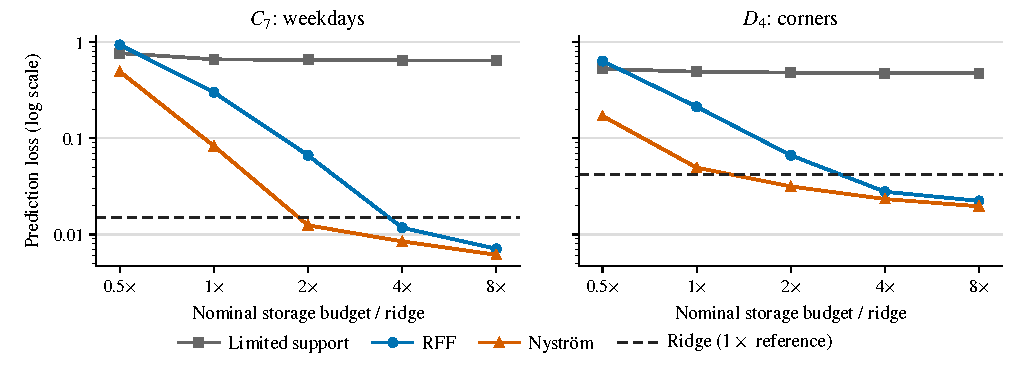
\includegraphics[width=\textwidth]{figures/budget_frontier.pdf}
\caption{\textbf{Predictor rankings change with storage.} Recorded direct-prediction means for all nonidentity actions on changed states under the specified semantic registration, over 24 fixed model/readout cells per domain. Losses use the Study~2 compact-comparison training-coordinate-energy denominator; lower is better. The horizontal axis is the nominal incremental parameter-storage budget relative to identity-pruned ridge, not runtime memory or statistical capacity. All five declared budgets and all three budgeted predictor families are shown. Nystr\"om first improves the group mean over ridge at $2\times$, and RFF at $4\times$, in both groups. Lines connect recorded aggregates on logarithmic axes; they are not fitted scaling laws or confidence bands. This direct-prediction endpoint is distinct from generator-only composition.}
\label{fig:budget-frontier}
\end{figure*}

\subsection{A transport advantage within the original construction}
Fitting context differences directly yields losses $0.03426/0.11639$ for $C_7/D_4$, versus $0.04714/0.13230$ for applying coordinate-fitted operators to those differences. The coherent action gives $0.03446/0.11717$ under the same direct fitting procedure and registration-specific scoring just described. Within that original bank, the improvement identifies a useful fitting objective; close means for distinct registered tasks establish neither semantic preference nor equivalence. Matched-state context differences cancel state means but retain context main effects, so this endpoint does not isolate state--context interactions. A fitted difference predictor also need not define a group action on the original coordinates. On jointly new $S_3$ contexts/entities, direct transport loss is $0.016290$ versus identity $0.016444$, a small absolute improvement below the inherited $0.01$ practical margin. Complete normalization and information conditions are in \cref{app:characterization,app:reproduction}. The new authored bank in \cref{tab:followup-context} tests this advantage under matched validation selection and reveals a domain-dependent reversal.

\paragraph{Behavioral scope.}
The activation-edit comparisons supply limited behavioral evidence: $C_7$ target logit improves over identity by 1.129, but the mean effect is smaller than that of the source-conditioned additive control. Correct $D_4$ ordering has lower final-logit distance than the matched wrong ordering. These are token/logit outcomes, not a certified native algorithm. The additive control uses full-hidden displacements and source identity, whereas the operator edits a PCA subspace; the mean-overwrite hook used in these comparisons lacks a matched zero-delta sham. The separate native program branch failed clean competence and its confirmation remains blocked. Full endpoints and limits, including the unchanged failure records, are in \cref{app:behavior,app:reproduction}.


\subsection{Detailed interpretation questions}
\label{app:detailed-reading-protocol}
The findings motivate four complementary questions, conditional on states, contexts, coordinates, estimator and outcome. They organize interpretation rather than define a calibrated certification test or four statistically independent sources of evidence.

\paragraph{1. Predictive recovery.}
State what was held out: contexts, action elements, state identities or domains. Disclose comparator supervision and storage. Our generator result demonstrates why the distinction matters: transfer to an excluded action element can still use a completely familiar state vocabulary.

\paragraph{2. Action consistency.}
Specify the group-law residual, its metric and whether fitting encouraged it. The propagation identity relates consistency to prediction errors and operator norms. To claim additional identification information, compare predictors under conditions that account for those quantities; independent objectives alone do not establish independent evidence.

\paragraph{3. Preferential semantic alignment.}
Compare coherent alternatives as well as invalid registrations, making information, capacity, scoring rows, target definitions and predictive difficulty explicit. Our comparisons show why these controls answer different questions. Preference over selected alternatives would narrow the interpretation, rather than identify a unique semantic mechanism.

\paragraph{4. Native causal use.}
For a claim about successful native computation, establish clean-task competence and intervention fidelity, then distinguish sufficiency from necessity for the proposed mechanism. These activation edits illustrate the gap between moving an output score and identifying the computation used by the unedited model.

For a new application, specify the intended claim and competing explanation before choosing a diagnostic. The useful outcome is the interpretation changed by the comparison, including unfavorable results, rather than the number of positive scores obtained.


\FloatBarrier
\section{Independent Orthogonality and Further Common-Law Cost}
\label{app:orthogonal-results}
This completed comparison adds a same-bank class optimum to the original spectral analysis. It separates the measured cost of independent orthogonality from bounds on the further cost of a common exact action. It uses the original canonical semantic registration only; no new state, context, model, alternative-image search or witness fit is introduced. The primary $r=16$ results and the completed spectral sensitivity remain unchanged. All full-precision endpoints, zero lower bounds and numerical checks are retained in the accompanying supplement and public project.

\subsection{Observation and numerical contract}
The panel contains 48 fixed model/readout/domain conditions at each of $r=16$ and $r=8$, for 96 units. Each test bank has 128 complete context blocks, with seven weekday or four corner states. Dimension eight takes the first eight columns of the saved training-PCA coordinates in their original order. Each dimension uses its own uncentered empirical second moment $\Sigma=Z^\top Z/N$ and symmetric inverse-square-root whitening. There is no extra recentering, PCA refit, new direction, jitter, pseudoinverse or rank reduction. States, context blocks and all group elements receive uniform weights; identity actions and fixed points are included.

The second moment must satisfy the original strict rule $\lambda_{\min}/\lambda_{\max}>10^{-10}$. Matrix identities use the original normalized Frobenius tolerance $10^{-8}$; scalar comparisons use $10^{-8}+10^{-7}\max(|a|,|b|)$. Singular values and risks are retained without clipping. The only clipping in the reported law interval is the mathematical definition $\ell^-=\max(0,L_{\rm lower}-L_{\rm orth})$. Original archive hashes, member identities, model/tokenizer revisions, PCA identities and complete state/template rows bind each input. The fixed runtime was Python 3.11 with NumPy 2.2.6.

For each action, compute $M_g=\mathbb E[x^\top x_g]$. If $M_g=U_g^{\rm svd}\operatorname{diag}(\sigma_{g,j})(V_g^{\rm svd})^\top$, one $O(r)$ optimum is $Q_g=U_g^{\rm svd}(V_g^{\rm svd})^\top$. No determinant correction is applied; the admissible class is $O(r)$, including reflections. A singular cross-moment may admit multiple optimal completions; the risk comparison does not identify a unique map. Direct residual risks are checked against
\[
 \eta=\frac{1}{r|G|}\sum_{g,j}(1-\sigma_{g,j}^2),\quad
 L_{\rm orth}=\frac{2}{r|G|}\sum_{g,j}(1-\sigma_{g,j}),\quad
 \beta=\frac{1}{r|G|}\sum_{g,j}(1-\sigma_{g,j})^2.
\]
These are optima on the complete bank used for their calculation, not training-fitted estimators scored on a different test distribution. The existing $\gamma_r$, $L_{\rm lower}$ and $L_{\rm upper}$ are read from authenticated saved endpoints. They are not re-estimated for this comparison. Independently computed $\eta$, identity risk and second-moment diagnostics must match the saved values under the original checks.

Eight numerical software fixtures passed before the completed analysis, covering an analytic nonzero orthogonality cost, an exact reflection, singular cross-moments, row-vector orientation, deficient moments and invalid weight/masking/nonfinite inputs. All 96 units then completed, with 11,520 recorded checks passing. The two source archives had identical hashes before and after execution. Those are implementation and preservation checks, not calibrated statistical tests or rigorous floating-point enclosures. This manuscript integration reads the completed outputs without repeating tests or analysis.

\subsection{Magnitude, concentration and zero lower endpoints}
\Cref{tab:core-risk-summary}b reports the saved equal-cell means. The quantities of interest are
\[
 L^\star-\eta=\beta+(L^\star-L_{\rm orth}),\qquad
 \ell^-=\max(0,L_{\rm lower}-L_{\rm orth}),\qquad
 \ell^+=L_{\rm upper}-L_{\rm orth}.
\]
Every $\ell^\pm$ is formed per cell before averaging. In particular, averaging a clipped endpoint differs from clipping a difference of domain means. The exact costs decompose additively, but $p^-$ need not equal $\beta+\ell^-$; dividing $\beta$ by the old lower bound $p^-$ does not estimate the proportion of true cost caused by orthogonality.

For $r=16$ C7, the additional-law lower endpoint has median $5.34554\times10^{-6}$ and range $[0,0.02618766]$. Its mean is $0.00109725$, and Llama-3.1-8B at layer 13 contributes $99.4445\%$ of its sum. The condition is retained at its original weight. This is concentration of the \emph{computed bounds}, not of the unknown true additional costs. It is a different quantity from the original joint lower endpoint $p^-$, whose sum has a $90.7\%$ contribution from two C7 conditions. For $r=16$ D4, the additional-law lower median is $0.000338944$ and the range is $[0,0.01261663]$; the largest condition contributes $28.5426\%$ of the sum. Upper bounds in both domains can remain much larger, so small lower bounds do not establish small optimal costs or practical equivalence.

At $r=8$, C7's additional-law lower median is $0.000778193$, with range $[0,0.11416052]$; D4's is $1.30864\times10^{-5}$, with range $[0,0.000401239]$. The smallest threshold-exceeding eight-coordinate C7 lower endpoint is $1.5462046788761175\times10^{-8}$, for Qwen2.5-3B at layer 7, only about $1.55$ times the unchanged software tolerance. It remains in the declared count; no threshold is adjusted retrospectively. These checks do not supply rigorous rounding-error certificates.

The nine zero lower endpoints are retained. At $r=16$ they occur for C7 in Llama-3.2-3B at layer 11, and for D4 in Qwen2.5-7B at layer 6. At $r=8$, the C7 cases are Qwen2.5-1.5B and Qwen2.5-7B at layer 6. The five D4 cases are Qwen2.5-7B at layer 22, Llama-3.1-8B at layer 13, Llama-3.2-1B at layer 13, and Llama-3.2-3B at layers 17 and 22. Zero is an inconclusive lower bound on strict positivity, not evidence that group laws have no cost. All 96 conditions remain in every relevant aggregate.

Each dimension changes the observation space, whitening and $1/r$ normalization. The two panels therefore do not select an optimal dimension or establish a common-metric improvement. The comparison concerns only the canonical action and does not rerank alternative images, re-evaluate frozen-witness transfer or add a semantic/native-computation claim. The full-precision table inputs, input mapping, checksums and formatting-only script are under \texttt{supplementary/orthogonal\_comparator}; complete per-cell summaries and the executed source bindings are retained in the public project.

\subsection{C7 context-family deletion sensitivity}
\label{app:c7-family-influence}
The concentration across model/readout conditions above does not establish concentration in a particular context family. We therefore examine whether removing any one family changes the additional-law lower bound in the original C7 bank. This completed, post-hoc analysis includes all 24 canonical-action conditions at $r=16$ and all 64 families. Each deletion removes both variants and their complete seven-state blocks, leaving 63 equally weighted families and 126 contexts. All states and all seven group elements, including identity, retain uniform weights. The original PCA basis, training mean, state correspondence, dimension and numerical tolerances remain fixed.

For each reduced bank, the unchanged spectral and independent-orthogonal kernels recompute its own \emph{uncentered} second moment and whitening, then evaluate $\eta$, $L_{\rm orth}$, $\gamma_r$ and the resulting constraint-cost bounds. Thus deletion changes both the empirical distribution and its metric, including the corresponding orthogonal-action class in the original coordinates. Differences are not additive family contributions under a fixed common metric. No extra centering, regularization, rank repair, historical-operator retraining or model forward pass is performed.

Twelve synthetic numerical tests passed, including closed-form risks, an independent Fourier-budget check, complete-family deletion and rank-failure cases. All 24 complete-bank baselines matched the saved results under the original rules before the 1,536 deletions were evaluated; all deletions completed. The analysis used Python 3.11.8 and NumPy 2.4.0, compared with NumPy 2.2.6 in the earlier orthogonal comparison. Baseline scalar discrepancies were at most $1.09\times10^{-14}$ without changing tolerances. The smallest reduced-bank second-moment eigenvalue ratio was $0.0039445$, above the original strict threshold $10^{-10}$. These are numerical validation checks, not rigorous floating-point certificates.

\begin{table}[t]
\centering\small
\setlength{\tabcolsep}{5pt}
\begin{tabular}{@{}lrrrrr@{}}
\toprule
Model & Layer & Baseline $\ell^-$ & Deletion min. & Deletion max. & \shortstack{Above tol.\\(/64)} \\
\midrule
Llama-3.2-1B & 3 & $3.540\times10^{-6}$ & $3.372\times10^{-6}$ & $4.079\times10^{-6}$ & 64/64 \\
 & 6 & $5.845\times10^{-6}$ & $5.252\times10^{-6}$ & $7.128\times10^{-6}$ & 64/64 \\
 & 10 & $1.128\times10^{-5}$ & $1.006\times10^{-5}$ & $1.374\times10^{-5}$ & 64/64 \\
 & 13 & $1.134\times10^{-5}$ & $1.047\times10^{-5}$ & $1.267\times10^{-5}$ & 64/64 \\
\addlinespace[2pt]
Llama-3.2-3B & 6 & $5.537\times10^{-6}$ & $5.307\times10^{-6}$ & $6.083\times10^{-6}$ & 64/64 \\
 & 11 & $0$ & $0$ & $0$ & 0/64 \\
 & 17 & $5.155\times10^{-6}$ & $4.104\times10^{-6}$ & $6.115\times10^{-6}$ & 64/64 \\
 & 22 & $2.595\times10^{-6}$ & $2.419\times10^{-6}$ & $2.914\times10^{-6}$ & 64/64 \\
\addlinespace[2pt]
Llama-3.1-8B & 6 & $2.058\times10^{-6}$ & $1.825\times10^{-6}$ & $2.406\times10^{-6}$ & 64/64 \\
 & 13 & $2.619\times10^{-2}$ & $2.435\times10^{-2}$ & $2.696\times10^{-2}$ & 64/64 \\
 & 19 & $6.538\times10^{-6}$ & $5.935\times10^{-6}$ & $7.448\times10^{-6}$ & 64/64 \\
 & 26 & $1.043\times10^{-5}$ & $9.416\times10^{-6}$ & $1.168\times10^{-5}$ & 64/64 \\
\addlinespace[2pt]
Qwen2.5-1.5B & 6 & $7.617\times10^{-6}$ & $7.267\times10^{-6}$ & $8.161\times10^{-6}$ & 64/64 \\
 & 11 & $1.238\times10^{-5}$ & $1.141\times10^{-5}$ & $1.370\times10^{-5}$ & 64/64 \\
 & 17 & $4.557\times10^{-6}$ & $4.209\times10^{-6}$ & $5.362\times10^{-6}$ & 64/64 \\
 & 22 & $6.010\times10^{-7}$ & $5.600\times10^{-7}$ & $7.323\times10^{-7}$ & 64/64 \\
\addlinespace[2pt]
Qwen2.5-3B & 7 & $6.462\times10^{-7}$ & $6.181\times10^{-7}$ & $7.216\times10^{-7}$ & 64/64 \\
 & 14 & $1.361\times10^{-5}$ & $1.127\times10^{-5}$ & $1.499\times10^{-5}$ & 64/64 \\
 & 22 & $2.747\times10^{-5}$ & $2.539\times10^{-5}$ & $2.914\times10^{-5}$ & 64/64 \\
 & 29 & $1.433\times10^{-6}$ & $1.342\times10^{-6}$ & $1.599\times10^{-6}$ & 64/64 \\
\addlinespace[2pt]
Qwen2.5-7B & 6 & $1.454\times10^{-6}$ & $9.852\times10^{-7}$ & $2.429\times10^{-6}$ & 64/64 \\
 & 11 & $6.239\times10^{-6}$ & $5.431\times10^{-6}$ & $7.513\times10^{-6}$ & 64/64 \\
 & 17 & $4.006\times10^{-6}$ & $3.560\times10^{-6}$ & $4.579\times10^{-6}$ & 64/64 \\
 & 22 & $1.933\times10^{-6}$ & $1.236\times10^{-6}$ & $2.487\times10^{-6}$ & 64/64 \\
\bottomrule
\end{tabular}

\caption{C7 family-deletion sensitivity of the further-law lower endpoint $\ell^-$, at $r=16$, in all 24 model/readout conditions. Minima and maxima cover all 64 complete-family deletions, each with its own empirical whitening; they are not confidence intervals. The final column counts endpoints satisfying $\ell^->10^{-8}+10^{-7}|\ell^-|$, out of 64. Zero is an inconclusive bound on strict positivity. Values are rounded only for display; full-precision endpoints and family identities are retained.}
\label{tab:c7-family-influence}
\end{table}

\Cref{tab:c7-family-influence} reports every condition. The same 23 conditions exceed the original tolerance after every deletion; Llama-3.2-3B/layer 11 retains a zero lower endpoint throughout. Across the 64 common-family deletions, the equal-cell mean $\ell^-$ ranges from $0.00102081$ to $0.00112915$, compared with $0.00109725$ on the complete bank; the mean upper endpoint ranges from $0.02970592$ to $0.03043969$. Llama-3.1-8B/layer 13 remains the largest contributor, with $\ell^-\in[0.02434807,0.02695796]$ versus $0.02618766$ originally. Deleting family 016 gives its largest reduction, about $7.02\%$; deleting family 044 gives its largest increase, about $2.94\%$. Its share of the lower-endpoint sum remains $99.3822\%$--$99.4776\%$. No single-family deletion removes this positive guarantee or the cross-condition concentration; neither statement measures the unknown true costs.

This sensitivity check supports stability to the declared single-family deletions, while leaving multiple-family effects and shared language-construction biases unresolved. It is not independent-context replication, population inference or evidence about native computation. It does not evaluate alternative registrations: the optional all-image registration LOFO described in \cref{app:bounded-margin-details} remains prepared and unexecuted. The source supplement under \texttt{supplementary/c7\_family\_influence\_v1} retains the complete scalar outputs, input mapping and table formatter; the public project also retains all per-deletion diagnostics and the unchanged executed code. This manuscript revision integrates those completed records without rerunning numerical tests or analysis.


\FloatBarrier
\section{Retained Spectral and Joint-Premium Summaries}
\label{app:retained-summaries}
The main text combines same-bank risks and constraint costs in \cref{tab:core-risk-summary}. For continuity with the complete cell-level results, this appendix retains the original separate spectral and joint-premium summaries. The numerical inputs, averaging weights and interpretations are unchanged. These tables use each original Study~2 test bank's own second-moment-whitened metric; they are distinct from the frozen-training-metric transfer comparison in \cref{tab:followup-witness}.

\begin{table}[t]
\centering\small
\begin{tabular}{@{}lrrrrr@{}}
\toprule
Domain & Mean $\gamma_r$ & Mean bound endpoints & Mean $\eta$ & Mean $b_{\rm triv}$ & Image rank 1 \\
\midrule
$C_7$ & 0.98510 & [0.02980, 0.05863] & 0.02563 & 0.61540 & 7/24 \\
$D_4$ & 0.93528 & [0.12944, 0.24895] & 0.10321 & 0.72742 & 16/24 \\
\bottomrule
\end{tabular}
\caption{Finite-bank exact-action bounds in the test-bank metric. Each domain has 24 model/readout cells at $r=16$. The bounds concern cell-specific $L^\star$ over the entire exact orthogonal-action class in each test bank's own second-moment-whitened metric; displayed endpoints average those bounds, not confidence limits. $b_{\rm triv}$ is selected trivial-type energy divided by $r$. The last column counts unique highest-$\gamma_r$ ranks of the specified image among 120 C7 or three D4 images; it is not a rank of exact $L^\star$ or a significance test.}
\label{tab:followup-spectral}
\end{table}


\begin{table}[t]
\centering\small
% Generated by analysis/main30_bounded_v1/derive.py; never edit numbers.
\begin{tabular}{lrrrr}
\toprule
Domain & Mean $\eta$ & Mean $L(I)$ & Mean $p^-$ & Mean $p^+$ \\
\midrule
C7 & 0.02563 & 0.76012 & 0.00416 & 0.03300 \\
D4 & 0.10321 & 0.52932 & 0.02624 & 0.14574 \\
\bottomrule
\end{tabular}

\caption{Same-metric reference and class-risk premium at $r=16$ on the original Study~2 test bank. Each domain averages \BoundedCellsPerDomain{} fixed cells equally. $p^-=\max\{0,2(1-\gamma_r)-\eta\}$ and $p^+=2(1-\gamma_r^2)-\eta$ are computed per cell before averaging. They bound the mean cost of imposing exact laws and orthogonality jointly. $L(I)$ uses total trivial energy and was also checked by direct residuals on the saved coordinates. These are finite-bank quantities, not transfer losses or confidence limits.}
\label{tab:bounded-risk}
\end{table}

\end{document}
